% Options for packages loaded elsewhere
\PassOptionsToPackage{unicode}{hyperref}
\PassOptionsToPackage{hyphens}{url}
%
\documentclass[
]{book}
\usepackage{lmodern}
\usepackage{amssymb,amsmath}
\usepackage{ifxetex,ifluatex}
\ifnum 0\ifxetex 1\fi\ifluatex 1\fi=0 % if pdftex
  \usepackage[T1]{fontenc}
  \usepackage[utf8]{inputenc}
  \usepackage{textcomp} % provide euro and other symbols
\else % if luatex or xetex
  \usepackage{unicode-math}
  \defaultfontfeatures{Scale=MatchLowercase}
  \defaultfontfeatures[\rmfamily]{Ligatures=TeX,Scale=1}
\fi
% Use upquote if available, for straight quotes in verbatim environments
\IfFileExists{upquote.sty}{\usepackage{upquote}}{}
\IfFileExists{microtype.sty}{% use microtype if available
  \usepackage[]{microtype}
  \UseMicrotypeSet[protrusion]{basicmath} % disable protrusion for tt fonts
}{}
\makeatletter
\@ifundefined{KOMAClassName}{% if non-KOMA class
  \IfFileExists{parskip.sty}{%
    \usepackage{parskip}
  }{% else
    \setlength{\parindent}{0pt}
    \setlength{\parskip}{6pt plus 2pt minus 1pt}}
}{% if KOMA class
  \KOMAoptions{parskip=half}}
\makeatother
\usepackage{xcolor}
\IfFileExists{xurl.sty}{\usepackage{xurl}}{} % add URL line breaks if available
\IfFileExists{bookmark.sty}{\usepackage{bookmark}}{\usepackage{hyperref}}
\hypersetup{
  pdftitle={数值分析笔记},
  pdfauthor={Xue Yu},
  hidelinks,
  pdfcreator={LaTeX via pandoc}}
\urlstyle{same} % disable monospaced font for URLs
\usepackage{color}
\usepackage{fancyvrb}
\newcommand{\VerbBar}{|}
\newcommand{\VERB}{\Verb[commandchars=\\\{\}]}
\DefineVerbatimEnvironment{Highlighting}{Verbatim}{commandchars=\\\{\}}
% Add ',fontsize=\small' for more characters per line
\usepackage{framed}
\definecolor{shadecolor}{RGB}{248,248,248}
\newenvironment{Shaded}{\begin{snugshade}}{\end{snugshade}}
\newcommand{\AlertTok}[1]{\textcolor[rgb]{0.94,0.16,0.16}{#1}}
\newcommand{\AnnotationTok}[1]{\textcolor[rgb]{0.56,0.35,0.01}{\textbf{\textit{#1}}}}
\newcommand{\AttributeTok}[1]{\textcolor[rgb]{0.77,0.63,0.00}{#1}}
\newcommand{\BaseNTok}[1]{\textcolor[rgb]{0.00,0.00,0.81}{#1}}
\newcommand{\BuiltInTok}[1]{#1}
\newcommand{\CharTok}[1]{\textcolor[rgb]{0.31,0.60,0.02}{#1}}
\newcommand{\CommentTok}[1]{\textcolor[rgb]{0.56,0.35,0.01}{\textit{#1}}}
\newcommand{\CommentVarTok}[1]{\textcolor[rgb]{0.56,0.35,0.01}{\textbf{\textit{#1}}}}
\newcommand{\ConstantTok}[1]{\textcolor[rgb]{0.00,0.00,0.00}{#1}}
\newcommand{\ControlFlowTok}[1]{\textcolor[rgb]{0.13,0.29,0.53}{\textbf{#1}}}
\newcommand{\DataTypeTok}[1]{\textcolor[rgb]{0.13,0.29,0.53}{#1}}
\newcommand{\DecValTok}[1]{\textcolor[rgb]{0.00,0.00,0.81}{#1}}
\newcommand{\DocumentationTok}[1]{\textcolor[rgb]{0.56,0.35,0.01}{\textbf{\textit{#1}}}}
\newcommand{\ErrorTok}[1]{\textcolor[rgb]{0.64,0.00,0.00}{\textbf{#1}}}
\newcommand{\ExtensionTok}[1]{#1}
\newcommand{\FloatTok}[1]{\textcolor[rgb]{0.00,0.00,0.81}{#1}}
\newcommand{\FunctionTok}[1]{\textcolor[rgb]{0.00,0.00,0.00}{#1}}
\newcommand{\ImportTok}[1]{#1}
\newcommand{\InformationTok}[1]{\textcolor[rgb]{0.56,0.35,0.01}{\textbf{\textit{#1}}}}
\newcommand{\KeywordTok}[1]{\textcolor[rgb]{0.13,0.29,0.53}{\textbf{#1}}}
\newcommand{\NormalTok}[1]{#1}
\newcommand{\OperatorTok}[1]{\textcolor[rgb]{0.81,0.36,0.00}{\textbf{#1}}}
\newcommand{\OtherTok}[1]{\textcolor[rgb]{0.56,0.35,0.01}{#1}}
\newcommand{\PreprocessorTok}[1]{\textcolor[rgb]{0.56,0.35,0.01}{\textit{#1}}}
\newcommand{\RegionMarkerTok}[1]{#1}
\newcommand{\SpecialCharTok}[1]{\textcolor[rgb]{0.00,0.00,0.00}{#1}}
\newcommand{\SpecialStringTok}[1]{\textcolor[rgb]{0.31,0.60,0.02}{#1}}
\newcommand{\StringTok}[1]{\textcolor[rgb]{0.31,0.60,0.02}{#1}}
\newcommand{\VariableTok}[1]{\textcolor[rgb]{0.00,0.00,0.00}{#1}}
\newcommand{\VerbatimStringTok}[1]{\textcolor[rgb]{0.31,0.60,0.02}{#1}}
\newcommand{\WarningTok}[1]{\textcolor[rgb]{0.56,0.35,0.01}{\textbf{\textit{#1}}}}
\usepackage{longtable,booktabs}
% Correct order of tables after \paragraph or \subparagraph
\usepackage{etoolbox}
\makeatletter
\patchcmd\longtable{\par}{\if@noskipsec\mbox{}\fi\par}{}{}
\makeatother
% Allow footnotes in longtable head/foot
\IfFileExists{footnotehyper.sty}{\usepackage{footnotehyper}}{\usepackage{footnote}}
\makesavenoteenv{longtable}
\usepackage{graphicx}
\makeatletter
\def\maxwidth{\ifdim\Gin@nat@width>\linewidth\linewidth\else\Gin@nat@width\fi}
\def\maxheight{\ifdim\Gin@nat@height>\textheight\textheight\else\Gin@nat@height\fi}
\makeatother
% Scale images if necessary, so that they will not overflow the page
% margins by default, and it is still possible to overwrite the defaults
% using explicit options in \includegraphics[width, height, ...]{}
\setkeys{Gin}{width=\maxwidth,height=\maxheight,keepaspectratio}
% Set default figure placement to htbp
\makeatletter
\def\fps@figure{htbp}
\makeatother
\setlength{\emergencystretch}{3em} % prevent overfull lines
\providecommand{\tightlist}{%
  \setlength{\itemsep}{0pt}\setlength{\parskip}{0pt}}
\setcounter{secnumdepth}{5}
\usepackage{booktabs}
\usepackage[]{natbib}
\bibliographystyle{apalike}

\title{数值分析笔记}
\author{Xue Yu}
\date{2020-04-28}

\begin{document}
\maketitle

{
\setcounter{tocdepth}{1}
\tableofcontents
}
\hypertarget{ux524dux8a00}{%
\chapter*{前言}\label{ux524dux8a00}}
\addcontentsline{toc}{chapter}{前言}

数值分析笔记。
用 R bookdown 写成。

\hypertarget{ux9ad8ux65afux6d88ux5143ux6cd5-gaussian-elimination}{%
\chapter{高斯消元法 \{Gaussian elimination\}}\label{ux9ad8ux65afux6d88ux5143ux6cd5-gaussian-elimination}}

这篇文章只是尝试把高斯消元法写的更清楚一点。

考虑方程:

\[
A \mathbf{x} = \mathbf{b}
\]

\(A \in R^{m \times n}, x \in R^n, b \in R^m\), 考虑A可逆,也就是以上方程只有唯一解。

\hypertarget{ux6570ux5b66}{%
\section{数学}\label{ux6570ux5b66}}

这实际上就是我们解矩阵方程组一般使用的方式,比如方程组是:

\[
a_{11}x_1 + a_{12}x_2 + \cdots + a_{1n}x_n = b_1 \\
a_{21}x_1 + a_{22}x_2 + \cdots + a_{2n}x_n = b_2 \\
\cdots \\
a_{m1}x_1 + a_{m2}x_2 + \cdots + a_{mn}x_n = b_m \\
\]

我们一般把它写成增广矩阵:

\[
\begin{bmatrix}
a_{11} & a_{12} &  \cdots &  a_{1n} & b_1 \\
a_{21} & a_{22} &  \cdots &  a_{2n} & b_2 \\
       &      \cdots    &      \\   
a_{m1} & a_{m2} &  \cdots &  a_{mn} & b_m \\
\end{bmatrix}
\]

首先化简成阶梯型矩阵的形式:

\begin{itemize}
\tightlist
\item
  \(row_1 / a_{11}\)
\item
  \(row_2 - k * row_1, k = \frac{a_{21}}{a_{11}}\)
\item
  \ldots{}
\end{itemize}

这样第一列就化为 \(\begin{bmatrix} 1 \\ \vdots \\ 0 \end{bmatrix}\)

对于第二列我们可以继续类似的操作:

\begin{itemize}
\tightlist
\item
  \(row_2 / (current)a_{22}\)
\item
  \(\cdots\)
\end{itemize}

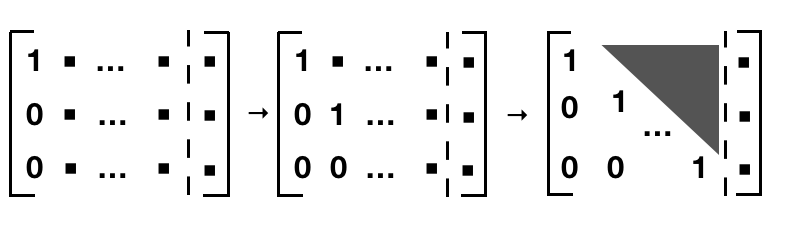
\includegraphics{images/Gauss_01_PLU_U.png}

经过这些操作矩阵A变成这样的一个上三角矩阵。 我们可以很容易的得到 \(x_m\) , 再往上回代就可以得到 \(x_1 \cdots x_m\):

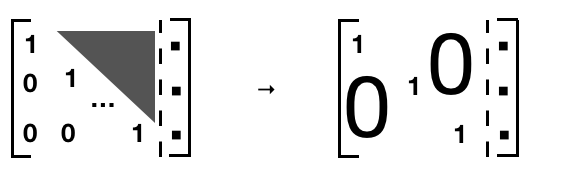
\includegraphics{images/Gauss_02_PLU_I.png}

\begin{itemize}
\tightlist
\item
  \(x_m\) get
\item
  \(row_{m-1} - k * row\)
\item
  \(\cdots\)
\end{itemize}

所以整个过程就只包括两个操作:

\begin{itemize}
\tightlist
\item
  \(row * k\)
\item
  \(row_j + row_i * k\)
\end{itemize}

我们也可以用另一种观点来看上述过程,其实也是三步:

\begin{itemize}
\tightlist
\item
  LU decomposition: A = LU ;
\item
  Forward substitution: solve Ly = b ;
\item
  Backward substitution: solve U x = y .
\end{itemize}

不过我们的前两步比较隐式和同时进行。

实际在计算机中计算,可能会出现的问题:

\begin{itemize}
\tightlist
\item
  \(a_{11}\) 为0,不能除0
\item
  \(a_{11} \ll 1\),除以一个很小很小的数会带来很多问题,比如overflow等
\end{itemize}

解决的办法就是行交换,把比较大的pivot放在前面。其实这个我们手动解 \(A\mathbf{x} = \mathbf{b}\) 的时候就会这样做,英文叫做 Gaussian elimination with partial pivoting (GEPP).

这里有一个具体的例子 \url{https://web.mit.edu/10.001/Web/Course_Notes/GaussElimPivoting.html}

这个英文就暗示了还有别的方法,因为这是 partial pivoting,还有一种 total pivoting,就是不仅仅只考虑行的交换,比如我们为了得到最大的\(a_{11}\), 我们也把列的交换也考虑上。

因为有行交换的原因,所以严格写会是:

\[
A = PLU
\]

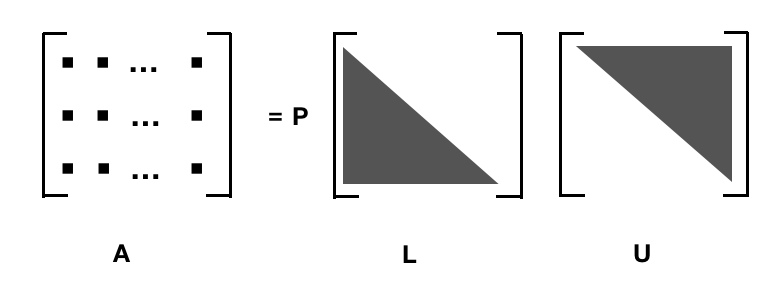
\includegraphics{images/Gauss_03_APLU.png}

同样也可以用另一种观点来看这个方法的正确性:

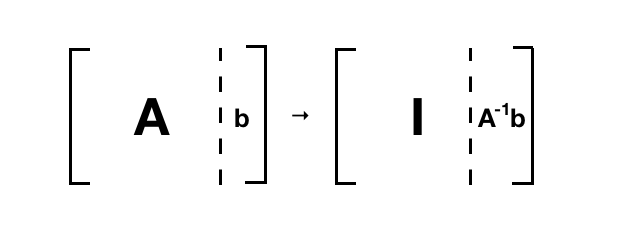
\includegraphics{images/Gauss_04_PLU_done.png}

不过我们并没有来算出 \(A^{-1}\)

\hypertarget{ux8ba1ux7b97}{%
\section{计算}\label{ux8ba1ux7b97}}

实际中,对于不是极其繁琐的有解线性方程组可以直接调库,比如直接用 \texttt{scipy.linalg.solve} 来帮助我们解方程, 一般来说,它会快于我们计算 \(A^{-1}\),然后 \(A^{-1}b\)。

计算

\[
\begin{cases}
2x_1 + 4x_2 - 2x_3 = 2 \\
x_1 - 3x_2 - 3x_3 = -1\\
4x_1 + 2x_2 + 2x_3 = 3
\end{cases}
\]

\begin{Shaded}
\begin{Highlighting}[]
\ImportTok{import}\NormalTok{ numpy }\ImportTok{as}\NormalTok{ np}
\ImportTok{from}\NormalTok{ scipy }\ImportTok{import}\NormalTok{ linalg}

\NormalTok{a }\OperatorTok{=}\NormalTok{ np.array([[}\DecValTok{2}\NormalTok{ ,}\DecValTok{4}\NormalTok{ ,}\OperatorTok{{-}}\DecValTok{2}\NormalTok{],}
\NormalTok{              [}\DecValTok{1}\NormalTok{, }\OperatorTok{{-}}\DecValTok{3}\NormalTok{, }\OperatorTok{{-}}\DecValTok{3}\NormalTok{],}
\NormalTok{              [}\DecValTok{4}\NormalTok{, }\DecValTok{2}\NormalTok{, }\DecValTok{2}\NormalTok{,]])}
\NormalTok{b }\OperatorTok{=}\NormalTok{ np.array([}\DecValTok{2}\NormalTok{, }\OperatorTok{{-}}\DecValTok{1}\NormalTok{, }\DecValTok{3}\NormalTok{])}

\NormalTok{x }\OperatorTok{=}\NormalTok{ linalg.solve(a, b)}
\NormalTok{np.dot(a, x) }\CommentTok{\# array([ 2., {-}1.,  3.])}
\NormalTok{x }\CommentTok{\# array([0.5       , 0.33333333, 0.16666667])}
\end{Highlighting}
\end{Shaded}

\begin{verbatim}
array([0.5       , 0.33333333, 0.16666667])
\end{verbatim}

我们的解答还是很接近数值解的:

\[
\begin{cases}
x_1 = 1/2 \\
x_2 = 1/3\\
x_3 = 1/6
\end{cases}
\]

更多操作,比如 lu 分解可以查看文档 \href{https://docs.scipy.org/doc/scipy-1.4.1/reference/generated/scipy.linalg.lu.html}{scipy.linalg.lu}

\hypertarget{choleskyux5206ux89e3-cholesky-decomposition}{%
\chapter{Cholesky分解 \{Cholesky decomposition\}}\label{choleskyux5206ux89e3-cholesky-decomposition}}

Cholesky 应该怎么念,o(╯□╰)o,听别人念比较像`瞅乐死骑',毕竟这是🇫🇷名字,哈哈哈哈

\hypertarget{ata}{%
\section{\texorpdfstring{\(A^{T}A\)}{A\^{}\{T\}A}}\label{ata}}

这个矩阵非常重要,之前在\href{https://zhuanlan.zhihu.com/p/89373759}{最小二乘法}也见过它,如果:

\[A\mathbf{x} = \mathbf{b}\]

无解,也就是 \(x= A^{-1}\mathbf{b}\) 不成立, A 不可逆,我们无法计算 \(A^{-1}\).

那么我们会想要最小化:

\[||A\mathbf{x} - \mathbf{b} ||_2\]

也就是:

\begin{align*}
|| A\mathbf{x} - \mathbf{b} ||^2 {}
&= (A\mathbf{x} - \mathbf{b})\cdot(A\mathbf{x} - \mathbf{b}) \\
&= (A\mathbf{x} - \mathbf{b})^T \cdot (A\mathbf{x} - \mathbf{b}) \\
&= (\mathbf{x}^TA^T - \mathbf{b}^T) \cdot (A\mathbf{x} - \mathbf{b})\\
&= (\mathbf{x}^TA^TA\mathbf{x} - 2\mathbf{b}^TA\mathbf{x} + \mathbf{b}^T\mathbf{b}) 
\end{align*}

这个 Error 函数对 \(\mathbf{x}\) 求导:

\[
\frac{\partial E}{\partial \mathbf{x}} =  2A^TA\mathbf{x} - 2 A^T \mathbf{b}= 0
\]

也就是需要解:

\[
A^TA\mathbf{x} = A^T \mathbf{b} \tag{1}
\]

(1)详细推导过程可以参见:\href{http://eeweb.poly.edu/iselesni/lecture_notes/least_squares/least_squares_SP.pdf}{least\_squares\_SP}

(1)式也就是:

\[
\mathbf{x} = (A^TA)^{-1} A^T \mathbf{b}  \tag{2}
\]

(1)式 一定可以推出 (2) 式么? \((A^TA)^{-1}\) 一定存在逆矩阵么?也许不一定,不一定的原因是比如 A 不是方阵,那么 \(A^TA\) 就可能只是半正定,所以逆矩阵不存在,所以才有\href{https://en.wikipedia.org/wiki/Tikhonov_regularization}{Tikhonov regularization}

\hypertarget{ux5bf9ux79f0}{%
\section{对称}\label{ux5bf9ux79f0}}

对称,首先 \(A^TA\) 是对称阵,记得 \((AB)^T = B^TA^T\):

\[(A^TA)^T  = A^T (A^T)^T = A^TA\]

它的转置等于自身,所以对称。

\hypertarget{ux6b63ux5b9aux77e9ux9635}{%
\section{正定矩阵}\label{ux6b63ux5b9aux77e9ux9635}}

先看定义:

\[
{\displaystyle M{\text{为正定矩阵}}\quad \iff \quad x^{\textsf {T}}Mx>0{\text{ for all }}x\in \mathbb {R} ^{n}\setminus \mathbf {0} }
\]

\[
{\displaystyle M{\text{为半正定矩阵}}\quad \iff \quad x^{\textsf {T}}Mx \ge 0{\text{ for all }}x\in \mathbb {R} ^{n}}
\]

这里的 A 我们暂时只考虑它是实数矩阵内,如果A是满秩的方阵,那么 \(A^TA\) 为正定矩阵:

\[x^TA^TAx = (Ax)^T \cdot Ax = ||Ax||^2\]

对于实正定矩阵,我们可以有Cholesky分解。

\hypertarget{choleskyux5206ux89e3}{%
\section{Cholesky分解}\label{choleskyux5206ux89e3}}

当 A 是一个SPD (real Symmetric positive definite matrix)的时候,注意这里的A 不是上面的 A(只是我用了同一个字母),就可以分解成 lower triangle 矩阵 L 和它的转置也就是 upper triangle \(L^T\).

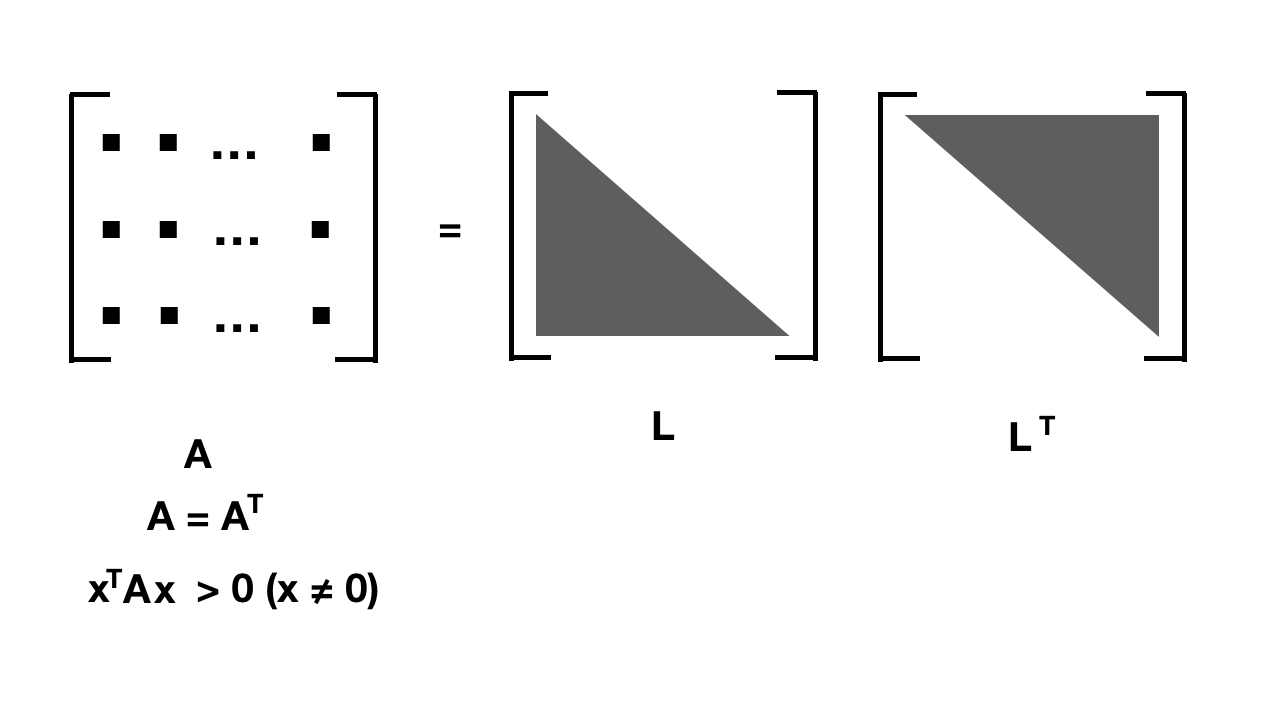
\includegraphics{images/Cholesky_ALL.png}

可以用归纳法证明这个分解是一定存在并且是唯一的,可以参见:

\href{https://math.stackexchange.com/questions/2509810/how-to-prove-the-existence-and-uniqueness-of-cholesky-decomposition}{How to prove the existence and uniqueness of Cholesky decomposition?}

之前的高斯消元法中我们写过:

\[
A = PLU
\]

当A正定的时候:

\[
A = LL^T
\]

在实际中,如果矩阵是正定的,使用 Cholesky分解 会比 LU分解 更加高效,更加数值稳定。

\hypertarget{ux8ba1ux7b97-1}{%
\section{计算}\label{ux8ba1ux7b97-1}}

\[
\begin{aligned}
\left({\begin{array}{*{3}{r}}4&12&-16\\12&37&-43\\-16&-43&98\\\end{array}}\right)=\left({\begin{array}{*{3}{r}}2&0&0\\6&1&0\\-8&5&3\\\end{array}}\right)\left({\begin{array}{*{3}{r}}2&6&-8\\0&1&5\\0&0&3\\\end{array}}\right)
\end{aligned}
\]

计算的话,我们可以用 \texttt{scipy.linalg.cholesky}

\begin{Shaded}
\begin{Highlighting}[]
\ImportTok{import}\NormalTok{ numpy }\ImportTok{as}\NormalTok{ np}
\ImportTok{from}\NormalTok{ scipy }\ImportTok{import}\NormalTok{ linalg}

\NormalTok{a }\OperatorTok{=}\NormalTok{ np.array([[}\DecValTok{4}\NormalTok{, }\DecValTok{12}\NormalTok{, }\OperatorTok{{-}}\DecValTok{16}\NormalTok{],}
\NormalTok{              [}\DecValTok{12}\NormalTok{, }\DecValTok{37}\NormalTok{, }\OperatorTok{{-}}\DecValTok{43}\NormalTok{],}
\NormalTok{              [}\OperatorTok{{-}}\DecValTok{16}\NormalTok{, }\OperatorTok{{-}}\DecValTok{43}\NormalTok{, }\DecValTok{98}\NormalTok{]])}
              
\NormalTok{L }\OperatorTok{=}\NormalTok{ linalg.cholesky(a, lower}\OperatorTok{=}\VariableTok{True}\NormalTok{) }\CommentTok{\# 默认计算 upper, 所以指定 lower = True}

\CommentTok{\# array([[ 2.,  0.,  0.],}
\CommentTok{\#       [ 6.,  1.,  0.],}
\CommentTok{\#       [{-}8.,  5.,  3.]])}

\NormalTok{np.allclose(np.dot(L, L.T) , a) }\CommentTok{\# 验证计算}
\end{Highlighting}
\end{Shaded}

\hypertarget{qr-ux5206ux89e3}{%
\chapter{QR 分解}\label{qr-ux5206ux89e3}}

任何的实方阵都可以做QR分解:

\[A = QR\]

其中 Q 是正交阵, R 是 upper triangle 矩阵.

Q 作为正交矩阵,有很多很好的特性:

\begin{itemize}
\tightlist
\item
  \(QQ^T = I\)
\item
  det(Q) = ±1, 如果 det(Q) = 1 则为旋转变换,说起旋转变换又会想到SO(n) 李群和李代数
\item
  可以给我们提供一组正交基
\end{itemize}

\hypertarget{gram-schmidt}{%
\section{Gram-Schmidt}\label{gram-schmidt}}

我们可以通过Gram--Schmidt来计算Q:

首先定义projection 操作:

\[\operatorname {proj} _{\mathbf {u} }\mathbf {a} ={\frac {\left\langle \mathbf {u} ,\mathbf {a} \right\rangle }{\left\langle \mathbf {u} ,\mathbf {u} \right\rangle }}{\mathbf {u} }\]

也就是把 \(\mathbf{a}\) 投影到 \(\mathbf{u}\) 方向上。

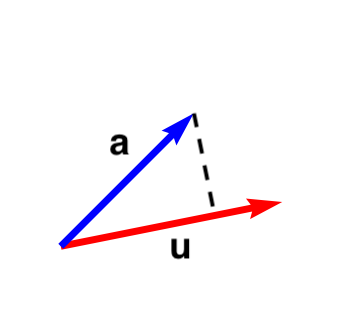
\includegraphics{images/QR_01_proj_v.png}

假设 \(A=\left[\mathbf {a} _{1},\ldots ,\mathbf {a} _{n}\right]\), 那么可以找到一组正交基:

\[
\begin{aligned}
\mathbf {u} _{1}&=\mathbf {a} _{1},&\mathbf {e} _{1}&={\mathbf {u} _{1} \over \|\mathbf {u} _{1}\|}\\\mathbf {u} _{2}&=\mathbf {a} _{2}-\operatorname {proj} _{\mathbf {u} _{1}}\,\mathbf {a} _{2},&\mathbf {e} _{2}&={\mathbf {u} _{2} \over \|\mathbf {u} _{2}\|}\\\mathbf {u} _{3}&=\mathbf {a} _{3}-\operatorname {proj} _{\mathbf {u} _{1}}\,\mathbf {a} _{3}-\operatorname {proj} _{\mathbf {u} _{2}}\,\mathbf {a} _{3},&\mathbf {e} _{3}&={\mathbf {u} _{3} \over \|\mathbf {u} _{3}\|}\\&\vdots &&\vdots \\\mathbf {u} _{k}&=\mathbf {a} _{k}-\sum _{j=1}^{k-1}\operatorname {proj} _{\mathbf {u} _{j}}\,\mathbf {a} _{k},&\mathbf {e} _{k}&={\mathbf {u} _{k} \over \|\mathbf {u} _{k}\|}
\end{aligned}
\]

A 可以表示为:

\[
\begin{aligned}
\mathbf {a} _{1}&=\langle \mathbf {e} _{1},\mathbf {a} _{1}\rangle \mathbf {e} _{1}\\\mathbf {a} _{2}&=\langle \mathbf {e} _{1},\mathbf {a} _{2}\rangle \mathbf {e} _{1}+\langle \mathbf {e} _{2},\mathbf {a} _{2}\rangle \mathbf {e} _{2}\\\mathbf {a} _{3}&=\langle \mathbf {e} _{1},\mathbf {a} _{3}\rangle \mathbf {e} _{1}+\langle \mathbf {e} _{2},\mathbf {a} _{3}\rangle \mathbf {e} _{2}+\langle \mathbf {e} _{3},\mathbf {a} _{3}\rangle \mathbf {e} _{3}\\&\vdots \\\mathbf {a} _{k}&=\sum _{j=1}^{k}\langle \mathbf {e} _{j},\mathbf {a} _{k}\rangle \mathbf {e} _{j}
\end{aligned}
\]

所以有:

\[Q=\left[\mathbf {e} _{1},\ldots ,\mathbf {e} _{n}\right]\]

\[
R = \begin{pmatrix}\langle \mathbf {e} _{1},\mathbf {a} _{1}\rangle &\langle \mathbf {e} _{1},\mathbf {a} _{2}\rangle &\langle \mathbf {e} _{1},\mathbf {a} _{3}\rangle &\ldots \\0&\langle \mathbf {e} _{2},\mathbf {a} _{2}\rangle &\langle \mathbf {e} _{2},\mathbf {a} _{3}\rangle &\ldots \\0&0&\langle \mathbf {e} _{3},\mathbf {a} _{3}\rangle &\ldots \\\vdots &\vdots &\vdots &\ddots \end{pmatrix}
\]

这个 R 为上三角矩阵由上面的计算过程看起来是一目了然,实际上我们动脑想一想也会觉得很清楚,因为 \(\mathbf{a}_{1}\) 定义了 \(\mathbf{e}_{1}\) ,而 \(\mathbf{a} _{2}\) 则完全由 \(\mathbf{e}_{1}, \mathbf{e}_{2}\) 确定, \(\mathbf{a}_{k}\) 只会由 \(\mathbf{e}_{1} \cdots \mathbf {e}_{k}\) 确定,所以当然就是上三角的。

不过实际上, Gram-Schmidt 计算方式并不是很数值稳定,想象一下矩阵:\(\begin{pmatrix} 1 & 1 + \varepsilon \\ 1 & 1\end{pmatrix}, \varepsilon \ll 1\),其实计算过程可能会出很大的问题。因为除以一个极小的数可能会带来很多无效数据。

\hypertarget{householderux53d8ux6362}{%
\section{Householder变换}\label{householderux53d8ux6362}}

projection 我们也可以写成矩阵形式:

\[\operatorname {proj} _{\mathbf {u} }\mathbf {a} ={\frac {\left\langle \mathbf {u} ,\mathbf {a} \right\rangle }{\left\langle \mathbf {u} ,\mathbf {u} \right\rangle }}{\mathbf {u} }\]

\[
\operatorname {proj} _{\mathbf {u} }\mathbf {a} = {\frac  {\mathbf {u}^T \cdot \mathbf {a} }{\mathbf {u}^T \cdot \mathbf {u} }} \cdot  {\mathbf {u} }  =  {\frac  { (\mathbf {u}^T \cdot \mathbf {a})  \cdot \mathbf {u}  }{\mathbf {u}^T \cdot \mathbf {u} }}
\]

点乘复合交换律和结合律,所以我们可以继续写成:

\[
\operatorname {proj} _{\mathbf {u} }\mathbf {a} =  {\frac  { \mathbf {u}\cdot \mathbf {u}^T  \cdot \mathbf {a}  }{\mathbf {u}^T \cdot \mathbf {u} }}
\]

这里 \(\mathbf {u}\cdot \mathbf {u}^T\) 是一个 3 x 3 的矩阵,所以

\[
P =  {\frac  { \mathbf {u}\cdot \mathbf {u}^T  }{\mathbf {u}^T \cdot \mathbf {u} }}
\]

又称作投影的矩阵形式。它本身也有一些特性,比如对称、比如\(P^2 = P\)\ldots.

接着来看反射操作:

\begin{figure}
\centering
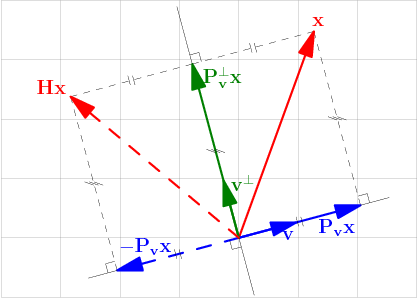
\includegraphics{images/QR_02_HouseholderReflection.png}
\caption{from wikipedia}
\end{figure}

\[
\begin{aligned}
\mathbf {b} - 2 \operatorname {proj} _{\mathbf {u} }\mathbf {b} {}
&= \mathbf {b} - 2 {\frac {\left\langle \mathbf {u} ,\mathbf {b} \right\rangle }{\left\langle \mathbf {u} ,\mathbf {u} \right\rangle }}{\mathbf {u} } \\
&= \mathbf {b} - 2 {\frac  { \mathbf {u}\cdot \mathbf {u}^T  }{\mathbf {u}^T \cdot \mathbf {u} }} \mathbf{b}\\
&=  ( I - 2 {\frac  { \mathbf {u}\cdot \mathbf {u}^T  }{\mathbf {u}^T \cdot \mathbf {u} })} \mathbf{b}\\
&= H_u\mathbf{b} 
\end{aligned}
\]

我们有反射矩阵:

\[
H_u = I - 2 {\frac  { \mathbf {u}\cdot \mathbf {u}^T  }{\mathbf {u}^T \cdot \mathbf {u} } } 
\]

为什么要引入这个反射矩阵?

wikipedia 上有关于这个矩阵的说法:

\begin{quote}
豪斯霍尔德变换可以将向量的某些元素置零,同时保持该向量的范数不变。

将非零列向量 \(\mathbf{x}=[x_1,\ldots,x_n ]^T\) 变换为单位基向量\(\mathbf{e}=[1,0,\ldots,0]^T\) 的豪斯霍尔德矩阵为

\(\mathbf{H} = \mathbf{I} - \frac{2}{\langle \mathbf{v},\mathbf{v} \rangle}\mathbf{vv}^H\)

其中豪斯霍尔德向量\(\mathbf{v}\)满足:

\(\mathbf{v} = \mathbf{x} + \rm{sign}(x_1) \Vert x \Vert_2 \mathbf{e}_1 . \,\)
\end{quote}

这个矩阵有特性包括:

\begin{itemize}
\tightlist
\item
  \(H^{T}=H\)
\item
  \(H^{-1}=H\)
\item
  \(H^{2}=I\)
\end{itemize}

假设 \(\mathbf{a}\) 是矩阵 A 的第一列, 有 \(H_u\) :

\[
c\mathbf{e}_1 = H_u \mathbf{a}
\]

也就做完这个操作可做到:

\[
\begin{pmatrix} x & x & x & x\\
x & x & x & x\\
x & x & x & x\\
x & x & x & x \end{pmatrix} \to
\begin{pmatrix} 1 & x & x & x\\
0 & x & x & x\\
0 & x & x & x\\
0 & x & x & x \end{pmatrix} 
\]

这就是我们高斯消元法做的第一步,这也是让我们朝着上三角迈进的第一步。 我们可以继续执行,最终我们可以得到上三角矩阵:

\[
R = H_{u_n} \cdots H_{u_1}A \\
Q = H_{u_1}^T \cdots H_{u_n}^T
\]

Gram-Schmidt 和 Householder 对于 \(A^{m \times n}\) 分解会有稍许不同:

\begin{itemize}
\tightlist
\item
  Gram-Schmidt : \(Q \in R^{m \times n}, R \in R^{n \times n}\)
\item
  Householder: \(Q \in R^{m \times m}, R \in R^{m \times n}\)
\end{itemize}

在计算中,Householder 的数值稳定性会稍优于 Gram-Schmidt.

\hypertarget{ux8ba1ux7b97-2}{%
\section{计算}\label{ux8ba1ux7b97-2}}

\[
A={\begin{pmatrix}12&-51&4\\6&167&-68\\-4&24&-41\end{pmatrix}}
\]

\[
Q={\begin{pmatrix}0.8571&-0.3943&0.3314\\0.4286&0.9029&-0.0343\\-0.2857&0.1714&0.9429\end{pmatrix}}\]

\[
R= \begin{pmatrix}14&21&-14\\0&175&-70\\0&0&-35\end{pmatrix}
\]

同样,QR 分解直接 \texttt{scipy.linalg.qr}:

\begin{Shaded}
\begin{Highlighting}[]
\ImportTok{import}\NormalTok{ numpy }\ImportTok{as}\NormalTok{ np}
\ImportTok{from}\NormalTok{ scipy }\ImportTok{import}\NormalTok{ linalg}

\NormalTok{a }\OperatorTok{=}\NormalTok{ np.array([[}\DecValTok{12}\NormalTok{, }\OperatorTok{{-}}\DecValTok{51}\NormalTok{, }\DecValTok{4}\NormalTok{],}
\NormalTok{              [}\DecValTok{6}\NormalTok{, }\DecValTok{167}\NormalTok{, }\OperatorTok{{-}}\DecValTok{68}\NormalTok{],}
\NormalTok{              [}\OperatorTok{{-}}\DecValTok{4}\NormalTok{, }\DecValTok{24}\NormalTok{, }\OperatorTok{{-}}\DecValTok{41}\NormalTok{]])}
              
\NormalTok{q, r }\OperatorTok{=}\NormalTok{ linalg.qr(a)}

\NormalTok{q}
\CommentTok{\# array([[{-}0.85714286,  0.39428571,  0.33142857],}
\CommentTok{\#       [{-}0.42857143, {-}0.90285714, {-}0.03428571],}
\CommentTok{\#       [ 0.28571429, {-}0.17142857,  0.94285714]])}

\NormalTok{r }
\CommentTok{\# array([[ {-}14.,  {-}21.,   14.],}
\CommentTok{\#       [   0., {-}175.,   70.],}
\CommentTok{\#       [   0.,    0.,  {-}35.]])}

\NormalTok{np.allclose(np.dot(q, r), a) }\CommentTok{\# True}
\end{Highlighting}
\end{Shaded}

符号不一样仅仅只是我们基 \(\mathbf{e}_1\cdots \mathbf{e}_n\) 的方向选择.

A = QR 的抗干扰性总觉得不是很好,即使A只有微小的变化,QR 也会剧烈改变。

\hypertarget{ux7279ux5f81ux5206ux89e3-eigen-decomposition}{%
\chapter{特征分解 \{Eigen decomposition\}}\label{ux7279ux5f81ux5206ux89e3-eigen-decomposition}}

\hypertarget{ux51faux73b0ux539fux56e0}{%
\section{出现原因}\label{ux51faux73b0ux539fux56e0}}

\hypertarget{ux4e3bux6210ux5206ux5206ux6790}{%
\subsection{主成分分析}\label{ux4e3bux6210ux5206ux5206ux6790}}

eigen是如此的重要,之前我已经写过一篇文章了\href{https://zhuanlan.zhihu.com/p/95836870}{特征值与特征向量},现在我们来看一下它可能会出现的场合,假设我有一堆 \(\mathbf{x}_i\), 我们想要找到它的主成分:

\begin{figure}
\centering
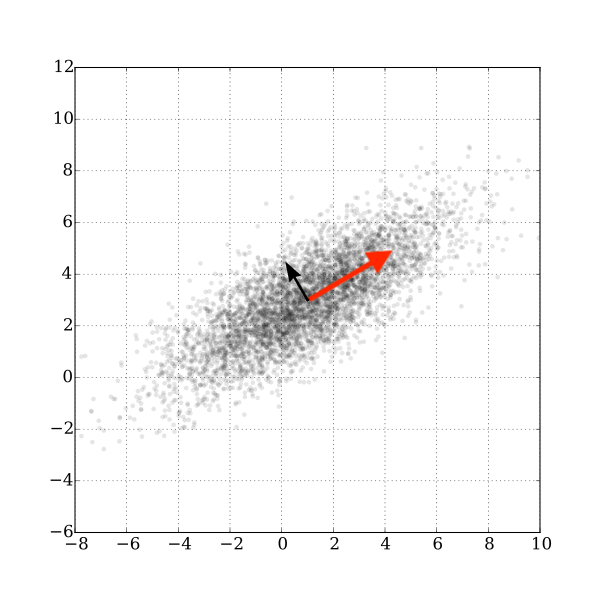
\includegraphics{images/GaussianScatterPCA.png}
\caption{图片来自wikipedia}
\end{figure}

比如就像图中,我们想找到红色箭头方向 \(\mathbf{v}_i\) ,那么我们可以列出方程:

\[
\text{minimize}  \sum_i || \mathbf{x}_i − \text{proj}_{\mathbf{v}} \mathbf{x}_i||^2 \\
|| \mathbf{v} || = 1
\]

加上 \(|| \mathbf{v} || = 1\) 假设 \(\mathbf{v}\) 为单位向量,方便计算,所以:

\[
\begin{aligned}
\sum|| \mathbf{x}_i − \text{proj}_{\mathbf{v}} \mathbf{x}_i||^2 {}
&= ||\mathbf{x}_i − (\mathbf{x}_i \cdot \mathbf{v})\mathbf{v}) ||^2 \\
&= ||\mathbf{x}_i||^2 - 2 (\mathbf{x}_i \cdot \mathbf{v})^2 +  (\mathbf{x}_i \cdot \mathbf{v})^2\\
&= ||\mathbf{x}_i||^2 - (\mathbf{x}_i \cdot \mathbf{v})^2\\
\end{aligned}
\]

最小化上面这个式子,其中 \(\mathbf{x}_i\) 是已知,我们要求 \(\mathbf{v}\) ,第一项固定,那么我们也就是最大化:

\[
\sum_i (\mathbf{x}_i \cdot \mathbf{v})^2
\]

那实际上也就是我们需要最大化:

\[
||X^T\mathbf{v}||^2\\
|| \mathbf{v} || = 1
\]

这里还是比较容易想清楚的,我们用 \(\mathbf{x}_i\) 来点乘 \(\mathbf{v}\), 然后要它们加起来和最大,每一项当然都要求大,我们就可以写成矩阵形式 \(X^T\mathbf{v}\), 而限制条件必不可少,单位向量是我们推导的前提 \(|| \mathbf{v} || = 1\), 否则没有这个限制最大化的话我们 \(\mathbf{v}\) 岂不是可以随便取大的。

最大化 \(||X^T\mathbf{v}||^2\) 也就是 最大化 \(\mathbf{v}^TXX^T\mathbf{v}\), 用格朗日乘数法,也就是

\[XX^T \mathbf{v} = \lambda \mathbf{v}\]

这个问题是求 \(XX^T\) 最大的 eigenvalue 的对应的 eigenvector.

\hypertarget{ux7269ux7406ux65b9ux7a0b}{%
\subsection{物理方程}\label{ux7269ux7406ux65b9ux7a0b}}

之前也写过, eigevalue, eigenvector 最早是为了解决微分方程出现的,比如最简单的考虑一个弹簧受力方程:

\[F = m \frac{d^2 \mathbf{x}}{dt} = -k \mathbf{x}\]

把微分算子写成 D:

\[
D^2 : f[\mathbf{x}] \to f[\mathbf{x}]\\
\mathbf{x} \mapsto D^2\mathbf{x} = \lambda \mathbf{x}
\]

\hypertarget{quadratic-energy}{%
\subsection{Quadratic Energy}\label{quadratic-energy}}

有时候我们会有这样的 setup(比如图像分割):

Have:

\begin{itemize}
\tightlist
\item
  n items in a dataset
\item
  \(w_{ij} ≥ 0\) similarity of items i and j
\item
  \(w_{ij} = w_{ji}\)
\end{itemize}

Want:
- \(x_{i}\) embedding on R

我们可以定义energy 方程:

\[
E(\mathbf{x}) = \sum_{ij} w_{ij} (x_i - x_j)^2
\]

我们想要最小化 \(E(\mathbf{x})\) 同时满足:

\[
||\mathbf{x}||^2 = 1 \\
\mathbf{1} \cdot \mathbf{x} = 0
\]

加上这些限制是为了防止最小值平凡的取为0.

用格朗日乘数法:

\[
\begin{aligned}
\Lambda &= \sum_{ij} w_{ij} (x_i - x_j)^2 - \lambda (\mathbf{x}^T \cdot \mathbf{x} - 1) - \mu (\mathbf{1} \cdot \mathbf{x}) {}
\end{aligned}
\]

最终化简为:

\[
E(\mathbf{x}) = \mathbf{x}^T(2A − 2W) \mathbf{x}
\]

最终我们需要找到的是: 矩阵 2A − 2W 对应的第二小的特征值的特征向量, 为什么不是最小的呢?因为大概最小的特征值是0,对应的可能也是 \(\mathbf{0}\).

这个对应的更多资料和证明可以参见:

\begin{itemize}
\item
  \href{https://www.cs.purdue.edu/homes/dgleich/demos/matlab/spectral/spectral.html}{Spectral Graph Partitioning and the Laplacian with Matlab}
\item
  \href{http://blog.shriphani.com/2015/04/06/the-smallest-eigenvalues-of-a-graph-laplacian/}{The Smallest Eigenvalues of a Graph Laplacian}
\end{itemize}

\hypertarget{ux5b9aux4e49}{%
\section{定义}\label{ux5b9aux4e49}}

\hypertarget{ux7279ux5f81ux503cux548cux7279ux5f81ux5411ux91cf}{%
\subsection{特征值和特征向量}\label{ux7279ux5f81ux503cux548cux7279ux5f81ux5411ux91cf}}

所以我们终于给出特征值和特征向量的定义了:

\[
A\mathbf{x} = \lambda \mathbf{x}\\
\lambda \in \mathbb{R} , A \in \mathbb{R}^{n \times n}
\]

对于复数:

\[
A\mathbf{x} = \lambda \mathbf{x}\\
\lambda \in \mathbb{C} , \mathbf{x} \in \mathbb{C}^n
\]

\(\lambda\) 是特征值, 而 \(\mathbf{x}\) 就是对应的特征向量

\hypertarget{ux8c31ux548cux8c31ux534aux5f84}{%
\subsection{谱和谱半径}\label{ux8c31ux548cux8c31ux534aux5f84}}

设 A 是 n × n 矩阵, 那么它的谱则是矩阵对应的特征向量。
而谱半径 ρ(A) 则是 \(\rho(A) = \max \left \{ |\lambda_1|, \cdots, |\lambda_n| \right \}\)

即矩阵A的谱半径等于矩阵A的特征值绝对值的最大值。 这句话好绕啊,还是看上面的数学式子比较明显。

\hypertarget{ux6709ux5173ux7279ux5f81ux503cux548cux7279ux5f81ux5411ux91cfux7684ux5b9aux7406}{%
\subsection{有关特征值和特征向量的定理}\label{ux6709ux5173ux7279ux5f81ux503cux548cux7279ux5f81ux5411ux91cfux7684ux5b9aux7406}}

\begin{itemize}
\tightlist
\item
  每个 \(A \in \mathbb{R}^{n \times n}\) 至少有一个(复) 特征向量
\item
  不同的特征值对应的特征向量一定是线性无关
\end{itemize}

所以当然 A 最多可以有 n 个不同的特征值,毕竟它最多 rank 也是n, 有 n 个线性无关的column vector。

\hypertarget{ux6269ux5c55ux5230ux590dux57df}{%
\subsection{扩展到复域}\label{ux6269ux5c55ux5230ux590dux57df}}

首先我们知道复数的 \(z = a + ib \in \mathbb{C}\) 的 共轭是 \(\bar{z} = a - ib\) 。

共轭转置是 A (m x n) 满足:

\[{\displaystyle \left({\boldsymbol {A}}^{\mathrm {H} }\right)_{ij}={\overline {{\boldsymbol {A}}_{ji}}}}   \]

以下写法都有:

\[{\boldsymbol {A}}^{\mathrm {H} }=\left({\overline {\boldsymbol {A}}}\right)^{\mathsf {T}}={\overline {{\boldsymbol {A}}^{\mathsf {T}}}}\]

埃尔米特矩阵( Hermitian) 矩阵是指:

\[{\displaystyle A{\text{ Hermitian}}\quad \iff \quad A= {A^H}}\]

埃尔米特矩阵的特征值都是实数,如果一个 A 只含实数,那么它是对称阵。

\begin{quote}
例如:
\end{quote}

\begin{quote}
\[{\begin{bmatrix}3&2+i\\2-i&1\end{bmatrix}}\]
\end{quote}

\begin{quote}
就是一个埃尔米特矩阵。
显然,埃尔米特矩阵主对角线上的元素都是实数的,其特征值也是实数。对于只包含实数元素的矩阵(实矩阵),如果它是对称阵,即所有元素关于主对角线对称,那么它也是埃尔米特矩阵。也就是说,实对称矩阵是埃尔米特矩阵的特例。
\end{quote}

对于埃尔米特矩阵, 不同的特征值对应的不同的特征向量它们之间一定是正交的。

\hypertarget{ux8c31ux5b9aux7406}{%
\subsection{谱定理}\label{ux8c31ux5b9aux7406}}

假设 \(A \in \mathbb{C}^{n \times n}\) 是一个 埃尔米特矩阵(如果\(A \in\mathbf{R}^{n \times n}\), 假设它对称既可)。那么, A 会有 n 个 正交的特征向量 \(\mathbf{x}_1, \cdots, \mathbf{x}_n\) ,它们对应的特征值(当然,可能会重复) 则是 \(\lambda_1,\cdots, \lambda_n\).

这里其实会有一点疑惑,那就是重复的特征值不带来重复的特征向量么? 为什么它们还是可以 span \(\mathbb{R}^n\)。

然后我就开始想,比如 \(I\) :

明显 \(I\) 有 n 个重复的 eigenvalue 1, 不过 \(I\) 是明显 span \(\mathbb{R}^n\) 的。

对于更一般的情况,貌似总可以用 Gram--Schmidt 来求出基。重复的 eigenvalue 的 eigenvector span 的是 plane, 而不是我想象的共线啊。o(╯□╰)o

这里有一个解答:

\href{https://math.stackexchange.com/questions/1517539/if-a-real-symmetric-matrix-has-repeated-eigenvalues-why-does-it-still-have-n-li/1517545\#1517545}{If a real symmetric matrix has repeated eigenvalues, why does it still have n linearly independent eigenvectors?}

谱定理非常重要,之前我多次写到过,比如\href{https://zhuanlan.zhihu.com/p/104079068}{傅里叶变换} 中我写到过,傅里叶级数其实也就是可以看成谱定理,无非是:

\begin{itemize}
\tightlist
\item
  把 \(\{1, \sin x, \cos x, \sin 2x, \cos2x, \cdots, \}\)看成空间中的基
\item
  然后展开成这组基的线性组合 \(f(x) = a_0/2 + \sum_{n = 1}^ \infty a_n \cos nx + b_n \sin nx\)
\end{itemize}

\hypertarget{ux7406ux8bbaux57faux7840}{%
\subsection{理论基础}\label{ux7406ux8bbaux57faux7840}}

再补充一点相关的理论基础:

\[A\mathbf{v} = \lambda \mathbf{v}\]

\[p(\lambda) = det(A - \lambda I) = 0\]

由代数基本定理(Fundamental theorem of algebra)我们知道 \(p(\lambda)\) 有 N 个解。这些解的解集也就是特征值的集合,有时也称为``谱''(Spectrum)。

\begin{quote}
代数基本定理: 任何一个非零的一元n次复系数多项式,都正好有n个复数根(重根视为多个根)。
\end{quote}

因式分解:

\[p\left(\lambda\right)= (\lambda-\lambda_1)^{n_1}(\lambda-\lambda_2)^{n_2}\cdots(\lambda-\lambda_k)^{n_k} = 0 \!\ \]

其中:

\[\sum\limits_{i=1}^{k}{n_i} =N\]

对每一个特征值 \(\lambda_i\) ,我们都有下式成立:

\[ \left(\mathbf{A} - \lambda_i \mathbf{I}\right)\mathbf{v}  = 0 \!\ \]

对每一个特征方程,都会有 \(m_i ( 1 \le m_i \le n_i)\) 个线性无关的解。这 \(m_i\) 个向量与一个特征值 \(\lambda_i\) 相对应。这里,整数 \(m_i\) 称为特征值 \(\lambda_i\) 的几何重数(geometric multiplicity),而 \(n_i\) 称为代数重数(algebraic multiplicity)。这里需要注意的是几何重数与代数重数可以相等,但也可以不相等。一种最简单的情况是 \(m_i = n_i = 1\)。\textbf{特征向量的极大线性无关向量组中向量的个数可以由所有特征值的几何重数之和来确定。}

这也是之前我们强调适用条件是 ``具有线性独立特征向量(不一定是不同特征值)的方阵 A'',也就是看 n x n 的方阵 A 是否可以特征分解主要是看几何重数之和是否为 n 了。

\hypertarget{ux8ba1ux7b97-3}{%
\section{计算}\label{ux8ba1ux7b97-3}}

之前的文章中当然也写到过一些计算和它们的推导,比如:

\[A^k\mathbf{x} = \lambda^k\mathbf{x}\]

如果 A 可逆:

\[A^{-1}\mathbf{x} =\frac{1}{\lambda} \mathbf{x}\]

再来看一些别的,比如我们的 setup 是:

\[ A \in \mathbb{R} ^{n \times n} \\
\mathbf{x}_1, \cdots, \mathbf{x}_n \in \mathbb{R}^n  \text{ eigenvector}  \\
|\lambda_1| \ge |\lambda_2| \ge \cdots \ge |\lambda_n| \text{ eigenvalues}
\]

根据谱定理,对于\(\mathbf{v} \in \mathbb{R}^n\), 我们有:

\[\mathbf{v} = c_1 \mathbf{x}_1 + \cdots + c_n\mathbf{x}_n\]

那么:

\[A^k\mathbf{v} = \lambda_1^k \bigg( c_1 \mathbf{x}_1 +  (\frac{\lambda_2}{\lambda_1})^k c_2 \mathbf{x}_2 + \cdots + (\frac{\lambda_n}{\lambda_1})^k  c_n\mathbf{x}_n \bigg)\]

\hypertarget{ux6700ux5927ux7684-eigenvalue-ux53caux5bf9ux5e94ux7684-eigenvector}{%
\subsection{最大的 eigenvalue 及对应的 eigenvector}\label{ux6700ux5927ux7684-eigenvalue-ux53caux5bf9ux5e94ux7684-eigenvector}}

如果 \(|\lambda_2| \le |\lambda_1|\) 有:

\[A^k \mathbf{v} = \lambda_1^k \mathbf{x}\]

所以比如我们取

\[\mathbf{v}_k = A \mathbf{v}_{k-1}\]

这样我们就可以算出来\textbf{最大的 eigenvalue 对应的 eigenvector},当然我们需要注意可能 \(|\lambda_1| \ge 1\),所以我们最好做一个 normalize 操作:

\[\mathbf{w}_k = A \mathbf{v}_{k-1}\\
\mathbf{v}_k = \frac{\mathbf{w}_k}{|\mathbf{w}_k|}
\]

这里的 norm 选哪个都所谓为,我们的重点只需要保证它不要无限制增长。

\hypertarget{ux6700ux5c0fux7684-eigenvalue-ux53caux5bf9ux5e94ux7684-eigenvector}{%
\subsection{最小的 eigenvalue 及对应的 eigenvector}\label{ux6700ux5c0fux7684-eigenvalue-ux53caux5bf9ux5e94ux7684-eigenvector}}

同样如果我们想要求出\textbf{最小的 eigenvalue 对应的 eigenvector} 我们可以这样操作:

\[\mathbf{w}_k = A^{-1} \mathbf{v}_{k-1}\\
\mathbf{v}_k = \frac{\mathbf{w}_k}{|\mathbf{w}_k|}
\]

因为 \(A^{-1}\) 的特征值满足:

\[|\frac{1}{\lambda_1}|  < |\frac{1}{\lambda_2}| < \cdots <|\frac{1}{\lambda_n}| \]

\hypertarget{ux9760ux8fd1-sigmaux7684-eigenvalue-ux53caux5bf9ux5e94ux7684-eigenvector}{%
\subsection{\texorpdfstring{靠近 \(\sigma\)的 eigenvalue 及对应的 eigenvector}{靠近 \textbackslash sigma的 eigenvalue 及对应的 eigenvector}}\label{ux9760ux8fd1-sigmaux7684-eigenvalue-ux53caux5bf9ux5e94ux7684-eigenvector}}

所以如果想要找到 \textbf{靠近 \(\sigma\)的 eigenvalue 的 eigenvector} :

\[\mathbf{v}_{k+1} = \frac{(A - \sigma I)^{-1} \mathbf{v}_k}{||(A - \sigma I)^{-1}\mathbf{v}_k||} \]

这个式子本质上跟上面找最小是一样的,我们是在找 \((A - \sigma I)\) 对应的最小的 eigenvector, 也就是这个 eigenvalue 需要靠近0, make sense.

\hypertarget{ux6839ux636e-eigenvector-ux731c-eigenvalue}{%
\subsection{根据 eigenvector 猜 eigenvalue}\label{ux6839ux636e-eigenvector-ux731c-eigenvalue}}

再来看一下问题的对立面,假设我们有一个 \(\mathbf{v}\) 非常靠近某个 eigenvector, 那么我们怎么求它对应的 eigenvalue 呢?

\[A\mathbf{v} \approx \lambda \mathbf{v}\]

这里我们要求的就是 \(\lambda\), 我们想做的就是:

\[
\text{arg min}_{\lambda}||A\mathbf{v} - \lambda \mathbf{v}||^2
\]

上面这个式子这种类型我们应该很熟悉了,展开,记住我们相求的是 \(\lambda\), 求导,最终可以写成是:

\[
\lambda = \frac{\mathbf{v}^T A \mathbf{v}}{||\mathbf{v}||^2}
\]

上面这个式子叫做 瑞利熵(Rayleigh quotient)。

它给了我们一种算法,叫做 瑞利商迭代(Rayleigh quotient iteration)。

\begin{enumerate}
\def\labelenumi{\arabic{enumi}.}
\item
  选择 \(\mathbf{v} \in R^n\) 为任意非零向量或者猜测一个特征向量。
\item
  迭代直至收敛:

  \begin{itemize}
  \tightlist
  \item
    计算对当前特征值的估计:\(\sigma_k = \frac{\mathbf{v}^T A \mathbf{v}}{||\mathbf{v}||^2}\)
  \item
    求解 \(\mathbf{w}_k = (A - \sigma I)^{-1} \mathbf{v}_{k-1}\)\\
  \item
    \(\mathbf{v}_k = \frac{\mathbf{w}_k}{|\mathbf{w}_k|}\)
  \end{itemize}
\end{enumerate}

wikipedia 上有一个具体的例子: \href{}{Rayleigh quotient iteration}

上面我们写了如何计算最大的 eigenvalue, 最小的eigenvalue, 或者最靠近 \(\sigma\) 的。

\hypertarget{all-eigenevalue}{%
\subsection{All eigenevalue}\label{all-eigenevalue}}

那么如何算出所有的 eigenvalue 呢?先回到这个式子:

\[\mathbf{v} = c_1 \mathbf{x}_1 + \cdots + c_n\mathbf{x}_n\]

那么如果我们找到了一个和 \(\mathbf{x}\) 垂直的向量 \(\mathbf{v}_0\)

\[\mathbf{v}_0\cdot \mathbf{x}_1 = 0\]

那么如果我们把 \(\mathbf{v}\) 在 \(\mathbf{x}_1\) 方向上的投影减去, 令之为 \(\mathbf{v}_1\)

\[\mathbf{v}_1 = c_2 \mathbf{x}_2 + \cdots + c_n\mathbf{x}_n\]

\[A\mathbf{v_1} = \lambda_2 \bigg( c_2 \mathbf{x}_2 + \cdots + (\frac{\lambda_n}{\lambda_2})  c_n\mathbf{x}_n \bigg)\\
A^k\mathbf{v_1} = \lambda_2^k \bigg( c_2 \mathbf{x}_2 + \cdots + (\frac{\lambda_n}{\lambda_2})^k  c_n\mathbf{x}_n \bigg)\]

这样不就可以继续算出 \(\mathbf{x}_2\) 了么?

这也提示了我们一种迭代法可以算出所有的 eigenvalue.

但是注意如果A 非对称,那么其特征向量不正交。

\textbf{但是这个算法的前提是 \(\mathbf{x}_1, \cdots, \mathbf{x}_n\) 这些特征向量之间是正交的}。

\textbf{对于任意矩阵,其对应于不同特征值的特征向量线性无关,但不一定正交,而对于实对称矩阵,其对应于不同特征值的特征向量是相互正交的。}

\hypertarget{householder-ux53d8ux6362}{%
\subsection{Householder 变换}\label{householder-ux53d8ux6362}}

如果A的特征向量不正交话我们可以用 Householder 变换配合来计算,假设我们有H如下:

\[H\mathbf{x}_1 = \mathbf{e}_1\]

\[
\begin{aligned}
HAH^T\mathbf{e}_1 {}
&= HAH\mathbf{e}_1 &H = H^T\\
&= HAHH\mathbf{x}_1 &H^2=I\\
&= HA\mathbf{x}_1 \\
&= \lambda_1H\mathbf{x}_1 \\
&= \lambda_1\mathbf{e}_1 \\
\end{aligned}
\]

所以:

\[
HAH^T = \begin{bmatrix}
\lambda_1 & b \\
0 & B
\end{bmatrix}
\]

所以利用 H 可以计算出 \(\lambda_1\), 不过后续的还要迭代继续。

\hypertarget{qr}{%
\subsection{QR}\label{qr}}

如果:

\[A = QR\\
Q^{-1} = Q^{T} \\
Q^{-1}AQ = Q^TAQ  = Q^T QR Q = RQ
\]

这也就给我们了一个迭代算法

\[
A_1 = A \\
A_k = Q_kR_k\\
A_{k+1} = R_kQ_k
\]

或者写成一句:

\[{\displaystyle A_{k+1}=R_{k}Q_{k}=Q_{k}^{-1}Q_{k}R_{k}Q_{k}=Q_{k}^{-1}A_{k}Q_{k}=Q_{k}^{\mathsf {T}}A_{k}Q_{k}}\]

\(A_k\) 系列总是相似的,有着相同的 eigenvalue, 而且这个方法具有数值稳定性。

具体参见: \href{https://en.wikipedia.org/wiki/QR_algorithm}{QR algorithm}

具体计算我们依旧可以用 \texttt{scipy.linalg} 模块,有众多函数可选,比如:

\begin{Shaded}
\begin{Highlighting}[]
\OperatorTok{\textgreater{}\textgreater{}\textgreater{}} \ImportTok{import}\NormalTok{ numpy }\ImportTok{as}\NormalTok{ np}
\OperatorTok{\textgreater{}\textgreater{}\textgreater{}} \ImportTok{from}\NormalTok{ scipy }\ImportTok{import}\NormalTok{ linalg}
\OperatorTok{\textgreater{}\textgreater{}\textgreater{}}\NormalTok{ a }\OperatorTok{=}\NormalTok{ np.array([[}\DecValTok{1}\NormalTok{, }\DecValTok{0}\NormalTok{], [}\DecValTok{1}\NormalTok{, }\DecValTok{3}\NormalTok{]])}
\OperatorTok{\textgreater{}\textgreater{}\textgreater{}}\NormalTok{ linalg.eigvals(a)}
\NormalTok{array([}\FloatTok{3.}\OperatorTok{+}\OtherTok{0.j}\NormalTok{, }\FloatTok{1.}\OperatorTok{+}\OtherTok{0.j}\NormalTok{])}
\end{Highlighting}
\end{Shaded}

\hypertarget{ux5947ux5f02ux503cux5206ux89e3-svd-decomposition}{%
\chapter{奇异值分解 \{SVD decomposition\}}\label{ux5947ux5f02ux503cux5206ux89e3-svd-decomposition}}

\hypertarget{ux5f15ux5165}{%
\section{引入}\label{ux5f15ux5165}}

首先我们来看 SVD 的引入(?证明(?,最直观的看法是比如我们想看变换 \(A\vec{x}\) 对向量 \(\vec{x}\) 造成的影响,至少我们来看对于模长的影响:

\[
R(\vec{x}) = \frac{\parallel A\vec{x}\parallel _2}{\parallel \vec{x}\parallel _2}
\]

首先可以注意的是:

\[
R(\alpha \vec{x}) = \frac{\parallel A \alpha \vec{x}\parallel _2}{\parallel \alpha \vec{x}\parallel _2} = \frac{\parallel \alpha\parallel  \cdot \parallel A  \vec{x}\parallel _2}{\parallel \alpha \parallel  \cdot \parallel \vec{x}\parallel _2} = \frac{\parallel A\vec{x}\parallel _2}{\parallel \vec{x}\parallel _2}
\]

\begin{itemize}
\tightlist
\item
  \(R(\alpha \vec{x}) = R(\vec{x})\) ,说明研究单位向量 \(\parallel \vec{x}\parallel _2 = 1\) 足矣
\item
  \(R(\vec{x}) \ge 0\), 研究 \(R^2(\vec{x})\) 也一样
\end{itemize}

来看一下对向量模缩放的极值,用朗格朗日乘子法:

\[
L(\vec{x}) = (A\vec{x})^2 - \lambda(\vec{x}^2 - 1)
\]

求导,看极值,依旧是我们熟悉的形式:

\[
(A^TA)\vec{x}_i = \lambda_i\vec{x}_i \tag{1}
\]

我们想要看 \(A\vec{x}\) 对 \(\vec{x}\) 的模的 影响,不过出现的极值对应的是 \(A^TA\) 的特征值 o(╯□╰)o

这个特殊的矩阵具有的性质包括:

\begin{itemize}
\tightlist
\item
  \(\lambda_i \ge 0 \forall i\), 这里很容易理解,因为 \(A^TA\) 是实对称的,是正定的
\item
  这个矩阵的基是一组完整的正交组
\end{itemize}

我们更想知道的是变换与 A 的关系。对于 \(A^TA\) 的特征向量 \(\vec{x}_i\), 考虑: \(\vec{y}_i = A \vec{x}_i\), 我们可以证明:

\textbf{\(\vec{y}_i\) 要么是 \(\vec{0}\), 要么是 \(AA^T\) 的特征向量。}

注意上面我们查看极值处出现的是 \(A^TA\), 而 \(\vec{y}\) 对应的是 \(AA^T\), 一般情况下,他们是不同的,一个很简单的问题就是比如 \(A \in \mathbb{R}^{m \times n}\), 那么 \(AA^T \in \mathbb{R}^{m \times m}\), \(A^TA \in \mathbb{R}^{n \times n}\).

又或者即使 \(A \in \mathbb{R}^{n \times n}\) 也容易肉眼验证 \(AA^T\) 和 \(A^TA\) 是不一样的:

\begin{verbatim}
>>> import numpy as np
>>> a = np.random.rand(3,3)
>>> a
array([[0.73741709, 0.2207241 , 0.60793118],
       [0.00490906, 0.18066958, 0.44795408],
       [0.70657397, 0.5650763 , 0.29043162]])
>>> aat = np.dot(a, a.T)
>>> aat
array([[0.96208341, 0.31582341, 0.82232812],
       [0.31582341, 0.23332846, 0.23566075],
       [0.82232812, 0.23566075, 0.90290852]])
>>> ata = np.dot(a.T, a)
>>> ata
array([[1.04305484, 0.56292085, 0.6557093 ],
       [0.56292085, 0.40067186, 0.37923277],
       [0.6557093 , 0.37923277, 0.6545937 ]])
>>> np.allclose(aat, ata)
False
>>> from scipy import linalg
>>> linalg.eigvals(aat)
array([1.84996505+0.j, 0.0737421 +0.j, 0.17461325+0.j])
>>> linalg.eigvals(ata)
array([1.84996505+0.j, 0.0737421 +0.j, 0.17461325+0.j])
\end{verbatim}

不过 \(AA^T\) 和 \(A^TA\) 的特征值看起来算出来一样,实际上这是一个可以推广的结论:

\textbf{\(A, B \in \mathbb{R}^{n \times n}, AB\) 和 \(BA\) 特征值一样}.

一个简单的证明如下:

\[AB\vec{x} = \lambda \vec{x}\]

令 \(\vec{y} = B\vec{x}\), 那么(当然我们这里考虑的都是 \(\lambda \ne 0, \vec{x} \ne 0\))

\[B A \vec{y} = BAB\vec{x} = B \lambda \vec{x} = \lambda B \vec{x} = \lambda \vec{y} \]

回到 \textbf{\(\vec{y}_i = A \vec{x}_i,\vec{y}_i\) 要么是 \(\vec{0}\), 要么是 \(AA^T\) 的特征向量。}

证明:

\[
\begin{aligned}
\lambda_i \vec{y_i} {}
&= \lambda_i A\vec{x_i}\\
&= A (\lambda_i \vec{x_i}) \\
&= A (A^TA \vec{x_i}) & \text{from (1)}\\ 
&= (AA^T) \vec{y}_i & \text{(2)} \\ 
\end{aligned} 
\]

所以 \(\vec{y}_i\) 是 \(AA^T\) 对应的特征向量,并且:

\[
\begin{aligned}
\parallel \vec{y_i}\parallel  {}
&= \parallel  A\vec{x_i}\parallel  \\
&= \sqrt{ \parallel  \lambda_i A\vec{x_i}\parallel  ^2}\\
&= \sqrt{ \vec{x}_i^T A^T A \vec{x}_i} \\
&= \sqrt{ \vec{x}_i^T A^T A \vec{x}_i} \\ 
&= \sqrt{ \vec{x}_i^T \lambda_i \vec{x}_i} & \text{from (1)} \\
&= \sqrt{  \lambda_i \vec{x}_i^T \vec{x}_i} \\
&= \sqrt{  \lambda_i} \parallel \vec{x}_i\parallel  \\
\end{aligned}
\]

如果 \(\lambda_i = 0, \vec{y}_i = \vec{0}\), 所以这就证明了我们的说法: \textbf{\(\vec{y}_i\) 要么是 \(\vec{0}\), 要么是 \(AA^T\) 的特征向量,并且 \(\parallel \vec{y_i}\parallel = \sqrt{ \lambda_i} \parallel \vec{x}_i\parallel\).}

现在我们继续 k 是 \(A^TA\) 大于 0 的特征值数量,对应的特征值是 \(\lambda_1, \cdots, \lambda_k\), 对应的特征向量是 \(\vec{x}_1, \cdots, \vec{x}_k \in \mathbb{R}^n\), 我们又知道 \(AA^T\) 和 \(A^TA\) 的特征值一样,所以有:

\[
k = \text{number of} \lambda_i > 0 \\
A^TA \vec{x}_i = \lambda_i \vec{x}_i \\
AA^T \vec{y}_i = \lambda_i \vec{y}_i \\
\]

我们假设 \(\parallel \vec{x}_i\parallel = 1\), 取

\[\vec{y}_i = \frac{1}{\sqrt{\lambda_i}} A \vec{x}_i  \tag{3}\]

可以证明:

\[
\parallel \vec{y}_i\parallel  = \frac{1}{\sqrt{\lambda}} \parallel A\vec{x}_i \parallel  = \frac{1}{\sqrt{\lambda}} \sqrt{\lambda} \parallel \vec{x}_i\parallel  = 1
\]

所以如果 \(\vec{x}_i\) 都是单位向量的话, \(\vec{y}_i\) 也是, 所以我们可以取

\[
\bar{V} = \begin{pmatrix} \vec{x}_1 & \cdots & \vec{x}_k \end{pmatrix}  \in \mathbb{R}^{n \times k} \\
\bar{U} = \begin{pmatrix} \vec{y}_1 & \cdots & \vec{y}_k \end{pmatrix} \in \mathbb{R}^{m \times k}
\]

令 \(\vec{e}_1\) 为第 i 个标准正交基向量,则:

\[
\begin{aligned}
\bar{U}^T A \bar{V} \vec{e}_1{} &=  \bar{U}^T A \vec{x}_i & \bar{V} \text{ defination} \\
&=  \frac{1}{\lambda_i} \bar{U}^T A (\lambda_i \vec{x}_i) \\
&= \frac{1}{\lambda_i} \bar{U}^T A (A^TA \vec{x}_i)  & \text{ from (1)} \\
&= \frac{1}{\lambda_i} \bar{U}^T (AA^T) A \vec{x}_i \\
&= \frac{1}{\sqrt{\lambda_i}} \bar{U}^T (AA^T) \vec{y}_i & \text{from (3)}\\ 
&= \frac{1}{\sqrt{\lambda_i}} \bar{U}^T \lambda_i \vec{y}_i & \text{from (2)}  \\
&= \sqrt{\lambda_i}  \bar{U}^T  \vec{y}_i \\
&= \sqrt{\lambda_i}\vec{e}_i \\
\end{aligned}
\]

令 \(\Sigma = diag (\sqrt{\lambda_1}, \cdots, \sqrt{\lambda_k})\),所以:

\[\bar{U}^T A \bar{V} = \Sigma\]

再回首看一下这个结论,那就是:

\[\bar{U} \in \mathbb{R}^{m \times k},  \bar{V} \in \mathbb{R}^{n \times k},  A \in \mathbb{R}^{m \times n}, \Sigma \in \mathbb{R}^{k \times k} \]

但是 \(\bar{U}, \bar{V}\) 不是方阵, 我们可以添加一些基,使得 \(A^TA\vec{x}_i = \vec{0}\) 和 \(AA^T\vec{y}_i = \vec{0}\), 这样 \(\bar{U}, \bar{V}\) 也就变成了方阵,满足:

\[\bar{U} \in \mathbb{R}^{m \times k},  \bar{V} \in \mathbb{R}^{n \times k}\mapsto U \in \mathbb{R}^{m \times m}, V \in \mathbb{R}^{n \times n} \]

同时 \(\Sigma\) 对角也会变成:

\[
\Sigma_{ij} = \begin{cases}
\sqrt{\lambda}_i & i = j, i \le k\\
0 & \text{otherwise}
\end{cases}
\]

这样我们可以写出:

\[A = U \Sigma V^T\]

\textbf{终于,至此我们推导出奇异值分解, \(A = U \Sigma V^T\), 我们没有给 A 加上任何条件,它无需对称、无需正定、无需是实数。这就是奇异值分解。}

方阵的奇异值分解:

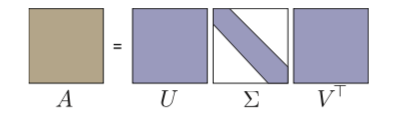
\includegraphics{images/svd_01.png}

非方阵的跟据我们上面的推导,可以写成这种紧凑型的:

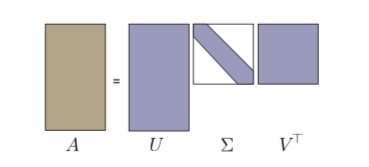
\includegraphics{images/svd_02.png}

也可以填0把 U、V 都写成方阵:

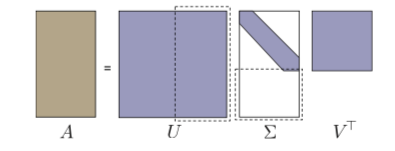
\includegraphics{images/svd_03.png}

\textbf{如果你拿到任何矩阵而毫无头绪,你总可以尝试奇异值分解。}

\hypertarget{ux7406ux89e3}{%
\section{理解}\label{ux7406ux89e3}}

\[A = U \Sigma V^T\]

\begin{itemize}
\tightlist
\item
  左奇异向量(left singular vector) : U 的列, span col A
\item
  右奇异向量(right singular vector): V 的列, span row A (注意这里是V而不是\(V^T\))
\item
  奇异值(singular value): \(\Sigma\) 的对角线,满足 \(\sigma_1 \ge \sigma_2 \cdots \ge 0\)
\end{itemize}

SVD = 方阵 x 对角阵 x 方阵, 一个方阵中包含了A的列向量的信息,另一个方阵中包含了A的行向量的信息。

其实我一直有一个疑惑就是为什么这个叫 singular value decompostion, 因为 non-invertable 的 矩阵也叫 singular 矩阵(invertible 也叫 nonsingular),查询后知道,原来singular 有几个意思: single(单个)、special(特别/不常见)的意思。

如果我们取 n x n 随机矩阵 R 的话,基本上都是不可逆的,用 singular 表示它处理起来比较麻烦,特别,当然你也可以记成它单身,找不到伴 \(R^{-1}\), 而 singular value decompostion 则一定就是 我们把这个矩阵做了特殊分解了吧,o(╯□╰)o

注意 特征分解 和 奇异分解 的不同:

\begin{quote}
这两种矩阵分解尽管有其相关性,但还是有明显的不同。对称阵特征向量分解的基础是谱分析,而奇异值分解则是谱分析理论在任意矩阵上的推广。
\end{quote}

为什么 SVD 这么引入注意?

因为我们可以把 SVD 这样来理解:

\begin{itemize}
\tightlist
\item
  \(V^T\) : 旋转
\item
  \(\Sigma\) : 缩放
\item
  U : 旋转
\end{itemize}

意思是任何矩阵\textbackslash 变换总可以看成 旋转 + 缩放 + 旋转。

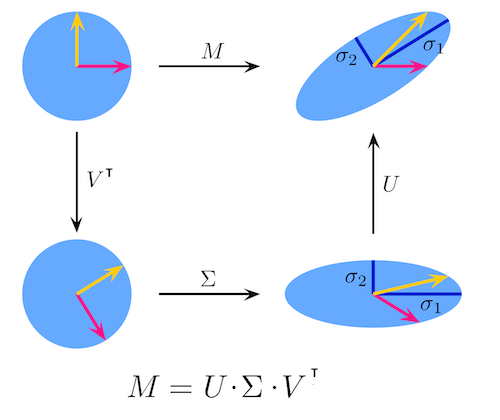
\includegraphics{images/svd_04.png}

\hypertarget{ux8ba1ux7b97-4}{%
\section{计算}\label{ux8ba1ux7b97-4}}

\begin{enumerate}
\def\labelenumi{\arabic{enumi}.}
\tightlist
\item
  V 是 \(A^TA\) 的特征向量
\item
  \(AV = U \Sigma\), 非0 奇异值对应的 \(\vec{u}_i\) 为 \(AV\) 标准化的列
\item
  \(AA^T\vec{u}_i = 0\) 可以解除剩下的
\end{enumerate}

\hypertarget{ux5e94ux7528}{%
\section{应用}\label{ux5e94ux7528}}

\hypertarget{ux4f8bux5b50ux4e00}{%
\subsection{例子一}\label{ux4f8bux5b50ux4e00}}

如果我们已经有了 A 的 SVD 分解,我们可以简化很多事:

\[A = U \Sigma V^T\]

我们可以相应知道 \(A^{-1}\), 当然前提 A 可逆(nonsingular 好绕):

\[
\begin{aligned}
A^{-1} {}
&=  (U \Sigma V^T)^{-1} \\
&= (V^T)^{-1} \Sigma^{-1} U^{-1} \\
&= V \begin{pmatrix} \sigma_1  & & \\ & \ddots &  \\  & & \sigma_n \end{pmatrix}^{-1} U^{-1} \\
&= V \begin{pmatrix} \frac{1}{\sigma_1}  & & \\ & \ddots &  \\  & & \frac{1}{\sigma_n} \end{pmatrix} U^T \\
\end{aligned}
\]

这个很容易解, 方阵的转置是它的逆, 对角的逆直接是它每个对角元素的倒数。

容易解\(A\vec{x}= \vec{b}\):

\[
\begin{aligned}
A\vec{x} {}
&= \vec{b} \\
U \Sigma V^T \vec{x} &= \vec{b}\\
\vec{x} &= V \Sigma^{-1} U^T \vec{b}  \\
\end{aligned}
\]

\hypertarget{ux4f8bux5b50ux4e8c}{%
\subsection{例子二}\label{ux4f8bux5b50ux4e8c}}

我们已经遇到过很多次这样的 setup 了:

\[
\text{minimize } \parallel \vec{x}\parallel _2^2 \\
\text{such that  } A^TA\vec{x} = A^T \vec{b}
\]

计算 \(A^TA\):

\[
\begin{aligned}
A^T A {}
&= (U \Sigma V^T)^T(U \Sigma V^T) \\
&= V \Sigma U^T U \Sigma V^T\\
&= V \Sigma^2 V^T \\
\end{aligned}
\]

所以 \(A^TA \vec{x} = A^T \vec{b}\) 可以写成:

\[
\begin{aligned}
A^TA \vec{x} = A^T \vec{b}  \iff V \Sigma^2 V^T \vec{x} &= (U \Sigma V^T)^T \vec{b}\\ {}
V \Sigma^2 V^T \vec{x} &= V \Sigma U^T \vec{b} \\
\Sigma V^T \vec{x} &=  U^T \vec{b}
\end{aligned}
\]

可以写成:

\[
\begin{aligned}
A^TA \vec{x} = A^T \vec{b}  \iff \Sigma \vec{y} &= \vec{d} \\ {}
\vec{y} &= V^T \vec{x} \\
\vec{d} &=  U^T \vec{b}
\end{aligned}
\]

上面的setup就可以改成:

\[
\text{minimize } \parallel \vec{y}\parallel _2^2 \\
\text{such that  } \Sigma \vec{y} =  \vec{d}
\]

\(\vec{y} = V^T \vec{x}\) 这个变换是一个旋转,所以当然对模长没有影响。

上面的 setup 由 \(\vec{x}\) 变成了 \(\vec{y}\), 那么有意思的地方也就出现了, \(\Sigma\) 是一个对角阵,所以:

\[
\begin{pmatrix} \sigma_1  & & \\ & \ddots &  \\  & & \sigma_k & \\ & & & 0 \end{pmatrix} 
\begin{pmatrix} y_1 \\  \vdots \\  \\  y_n \end{pmatrix} 
= \begin{pmatrix} d_1 \\ \vdots  \\ \\ d_m\end{pmatrix}
\]

所以可以设置:

\[
\Sigma_{ij}^+ =  \begin{cases}
\frac{1}{\sigma}_i & i = j, \sigma_i \ne 0,  i \le k\\
0 & \text{otherwise}
\end{cases} \\
\implies \vec{y} = \Sigma_{ij}^+ \vec{d} \\
\implies \vec{x} = V \Sigma_{ij}^+ U^T \vec{b}
\]

这个矩阵 \(V \Sigma_{ij}^+ U^T\) 还有一个专门的名字: Pseudoinverse(伪逆?),它有一些性质 :

\begin{itemize}
\tightlist
\item
  A square and invertible ⇒ \(A^+ = A^{−1}\)
\item
  A overdetermined ⇒ \(A^+\vec{b}\) gives least-squares solution to \(A\vec{x} = \vec{b}\)
\item
  A underdetermined ⇒\(A^+\vec{b}\) gives least-squares solution to \(A\vec{x} = \vec{b}\) with least (Euclidean) norm
\end{itemize}

\hypertarget{ux4f8bux5b50ux4e09}{%
\subsection{例子三}\label{ux4f8bux5b50ux4e09}}

A 的另一种写法:

\[A = U \Sigma V^T \implies A = \sum_{i = 1}^l \sigma_i \vec{u}_i \vec{v}_i^T\\
l = \text{min}\{ m, n\}\]

上面这种看法/写法很有意思。我们把 A 看成是 列向量 x 行向量 的和。

注意 \(\vec{u} \vec{v}^T\) 又被定义为外积:

\[\vec{u} \otimes \vec{v} = \vec{u} \vec{v}^T\]

计算 \(A\vec{x}\) :

\[A\vec{x} = \sum_i \sigma_i (\vec{v}_i \cdot \vec{x}) \vec{u}_i\]

这个写法给我们一些提示,那就是计算 \(A\vec{x}\) 我们可以 忽略很小的 \(\sigma_i\)

同时 \(A^+\vec{x}\) 可以:

\[A^+ = \sum_{\sigma_i \ne 0} \frac{\vec{v}_i \cdot \vec{u}^T}{\sigma_i }\]

计算 \(A^+\) 可以忽略 很大的 \(\sigma_i\)

实际上有个定理 \textbf{Eckart-Yound Theorem(低维矩阵近似)}:

\begin{quote}
Suppose \(\widetilde{A}\) is obtained from \(A = U\Sigma V^T\) by truncating all but the k largest singular values \(\sigma_i\) of A to zero. Then,\(\widetilde{A}\) minimizes both
\(\parallel A - \widetilde{A} \parallel _{Fbo}\) and \(\parallel A - \widetilde{A} \parallel _2\) subject to the constraint that the column space of \(\tilde{A}\) has at most dimension k.
\end{quote}

意思就是 从 A 找到一个 rank 为 r 的矩阵 \(\widetilde{A}\), 这个矩阵可以最小化与 A 之间的 Frobenius norm 和 2-norm, 这个 \(\widetilde{A}\) 是如何找到的呢? 就是我们用 SVD 将 A 分解成 \(A = U\Sigma V^T\) , 人然后 \(\Sigma\) 中最 k 个最大的 非0 奇异值。

Frobenius norm 的定义是:

\[
{\displaystyle \|A\|_{\text{F}}={\sqrt {\sum _{i=1}^{m}\sum _{j=1}^{n}|a_{ij}|^{2}}}={\sqrt {\operatorname {trace} \left(A^{*}A\right)}}={\sqrt {\sum _{i=1}^{\min\{m,n\}}\sigma _{i}^{2}(A)}}}
\]

这样当然是最小化啦,

2-norm 对矩阵的定义是:

\[{\displaystyle \parallel A\parallel _2 = \max _{{\vec {v}}\neq {\vec {0}}}{\frac {\parallel A{\vec {v}}\parallel _{2}}{\parallel {\vec {v}}\parallel _{2}}}} = \text{max} \{ \sigma_i \}\]

这也很容易理解,因为\(A = U \Sigma V^T\) 旋转,缩放 ,旋转, 改变长度的只有缩放\(\Sigma\), 而\(\sigma_i \ge 0\) 这个又是很显然的。(The singular values are non-negative real numbers.) 这个显然可以显然在上面的引入部分 \(\Sigma = diag (\sqrt{\lambda_1}, \cdots, \sqrt{\lambda_k})\)

实际上我们的奇异值也 \$A\^{}TA \$ 的特征根开根号, 而 \(A^TA\) 为正定,所以必定奇异值非负。

\hypertarget{ux4f8bux5b50}{%
\section{例子}\label{ux4f8bux5b50}}

考虑 M:

\[\mathbf {M} ={\begin{bmatrix}1&0&0&0&2\\0&0&3&0&0\\0&0&0&0&0\\0&2&0&0&0\end{bmatrix}}\]

对 M 做 奇异值分解的话: \(UΣV^*\):

\[
U = \begin{bmatrix} 0 & -1 & 0 & 0 \\ -1 & 0 & 0 & 0 \\ 0 & 0 & 0 & -1 \\ 0 & 0 & -1 & 0\end{bmatrix} \\
\Sigma = \begin{bmatrix} 3 & 0 & 0 & 0 & 0 \\ 0 & \sqrt{5} & 0 & 0 & 0 \\ 0 & 0 & 2 & 0 & 0 \\ 0 & 0 & 0 & 0 & 0\end{bmatrix}  \\
V^* = \begin{bmatrix} 0 & 0 & -1 & 0 & 0 \\ -\sqrt{0.2} & 0 & 0 & 0 & -\sqrt{0.8} \\ 0 & -1 & 0 & 0 & 0 \\ 0 & 0 & 0 & 1 & 0  \\ -\sqrt{0.8} & 0 & 0 & 0 & \sqrt{0.2} \end{bmatrix} \\
\]

\begin{Shaded}
\begin{Highlighting}[]
\OperatorTok{\textgreater{}\textgreater{}\textgreater{}} \ImportTok{from}\NormalTok{ scipy }\ImportTok{import}\NormalTok{ linalg}
\OperatorTok{\textgreater{}\textgreater{}\textgreater{}} \ImportTok{import}\NormalTok{ numpy }\ImportTok{as}\NormalTok{ np}
\OperatorTok{\textgreater{}\textgreater{}\textgreater{}}
\OperatorTok{\textgreater{}\textgreater{}\textgreater{}}\NormalTok{ a }\OperatorTok{=}\NormalTok{ np.array([[}\DecValTok{1}\NormalTok{, }\DecValTok{0}\NormalTok{, }\DecValTok{0}\NormalTok{, }\DecValTok{0}\NormalTok{, }\DecValTok{2}\NormalTok{],}
\NormalTok{...               [}\DecValTok{0}\NormalTok{, }\DecValTok{0}\NormalTok{, }\DecValTok{3}\NormalTok{, }\DecValTok{0}\NormalTok{, }\DecValTok{0}\NormalTok{],}
\NormalTok{...               [}\DecValTok{0}\NormalTok{, }\DecValTok{0}\NormalTok{, }\DecValTok{0}\NormalTok{, }\DecValTok{0}\NormalTok{, }\DecValTok{0}\NormalTok{],}
\NormalTok{...               [}\DecValTok{0}\NormalTok{, }\DecValTok{2}\NormalTok{, }\DecValTok{0}\NormalTok{, }\DecValTok{0}\NormalTok{, }\DecValTok{0}\NormalTok{]])}
\OperatorTok{\textgreater{}\textgreater{}\textgreater{}}
\OperatorTok{\textgreater{}\textgreater{}\textgreater{}}\NormalTok{ u, s, vh }\OperatorTok{=}\NormalTok{ linalg.svd(a)}
\OperatorTok{\textgreater{}\textgreater{}\textgreater{}}
\OperatorTok{\textgreater{}\textgreater{}\textgreater{}}\NormalTok{ u}
\NormalTok{array([[ }\FloatTok{0.}\NormalTok{,  }\FloatTok{1.}\NormalTok{,  }\FloatTok{0.}\NormalTok{,  }\FloatTok{0.}\NormalTok{],}
\NormalTok{       [ }\FloatTok{1.}\NormalTok{,  }\FloatTok{0.}\NormalTok{,  }\FloatTok{0.}\NormalTok{,  }\FloatTok{0.}\NormalTok{],}
\NormalTok{       [ }\FloatTok{0.}\NormalTok{,  }\FloatTok{0.}\NormalTok{,  }\FloatTok{0.}\NormalTok{, }\OperatorTok{{-}}\FloatTok{1.}\NormalTok{],}
\NormalTok{       [ }\FloatTok{0.}\NormalTok{,  }\FloatTok{0.}\NormalTok{,  }\FloatTok{1.}\NormalTok{,  }\FloatTok{0.}\NormalTok{]])}
\OperatorTok{\textgreater{}\textgreater{}\textgreater{}}\NormalTok{ s}
\NormalTok{array([}\FloatTok{3.}\NormalTok{        , }\FloatTok{2.23606798}\NormalTok{, }\FloatTok{2.}\NormalTok{        , }\FloatTok{0.}\NormalTok{        ])}
\OperatorTok{\textgreater{}\textgreater{}\textgreater{}}\NormalTok{ vh}
\NormalTok{array([[}\OperatorTok{{-}}\FloatTok{0.}\NormalTok{        ,  }\FloatTok{0.}\NormalTok{        ,  }\FloatTok{1.}\NormalTok{        , }\OperatorTok{{-}}\FloatTok{0.}\NormalTok{        ,  }\FloatTok{0.}\NormalTok{        ],}
\NormalTok{       [ }\FloatTok{0.4472136}\NormalTok{ ,  }\FloatTok{0.}\NormalTok{        ,  }\FloatTok{0.}\NormalTok{        ,  }\FloatTok{0.}\NormalTok{        ,  }\FloatTok{0.89442719}\NormalTok{],}
\NormalTok{       [}\OperatorTok{{-}}\FloatTok{0.}\NormalTok{        ,  }\FloatTok{1.}\NormalTok{        ,  }\FloatTok{0.}\NormalTok{        , }\OperatorTok{{-}}\FloatTok{0.}\NormalTok{        ,  }\FloatTok{0.}\NormalTok{        ],}
\NormalTok{       [ }\FloatTok{0.}\NormalTok{        ,  }\FloatTok{0.}\NormalTok{        ,  }\FloatTok{0.}\NormalTok{        ,  }\FloatTok{1.}\NormalTok{        ,  }\FloatTok{0.}\NormalTok{        ],}
\NormalTok{       [}\OperatorTok{{-}}\FloatTok{0.89442719}\NormalTok{,  }\FloatTok{0.}\NormalTok{        ,  }\FloatTok{0.}\NormalTok{        ,  }\FloatTok{0.}\NormalTok{        ,  }\FloatTok{0.4472136}\NormalTok{ ]])}
\end{Highlighting}
\end{Shaded}

可以看到这个用 scipy 来解 u 和 vh 跟上面有点区别,就是选择的方向的原因,o(╯□╰)o

\hypertarget{ux5947ux5f02ux503cux5206ux89e3ux7684ux5e94ux7528-svd-application}{%
\chapter{奇异值分解的应用 \{SVD application\}}\label{ux5947ux5f02ux503cux5206ux89e3ux7684ux5e94ux7528-svd-application}}

这里再写一些 SVD 更为具体的应用。

\hypertarget{rigid-alignment-procrustes-problem}{%
\section{Rigid Alignment / Procrustes Problem}\label{rigid-alignment-procrustes-problem}}

顾名思义, 比如我们想要这两个形状对齐:

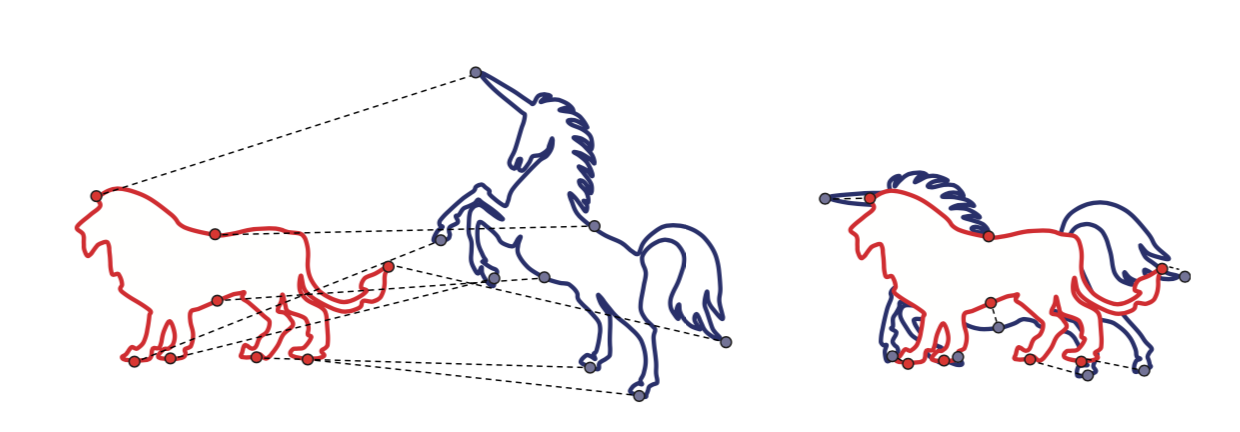
\includegraphics{images/rigid_alignment_01.png}

或者比如我们有两个点云,想让它们尽量对齐:

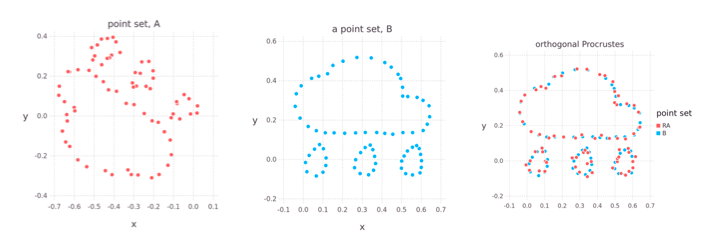
\includegraphics{images/rigid_alignment_02.png}

又或者我们3D扫描了一些点云,想要把它们对齐以生成更好的3D point clouds,最终生成更好的 3D mesh,也要用到 Rigid Alignment.

最简单的set up 就是我们有如上图的两个点云, 然后通过平移和旋转,最小化它们之间的距离:

\[
E  = \sum_{i=1}^n \parallel p_i-(Rq_i+  t) \parallel^2 \\
p_i \in P \\
q_i \in Q
\]

平移很容易求到, 让它们的质心重合:

\[
p = \frac{1}{n}\sum_{i=1}^np_i = \frac{1}{n}\sum_{i=1}^n (Rq_i+t) = R \frac{1}{n}\sum_{i=1}^nq_i + t = Rq + t \\
t = p - Rq
\]

质心重合之后我们就只需要最小化对应点之间的距离:

\[
\begin{aligned}
\sum_{i=1}^n \parallel p_i-(Rq_i+t) \parallel^2 &= \sum_{i=1}^n \parallel p_i - Rq_i - (p - Rq) \parallel^2 \\ 
    &= \sum_{i=1}^n \parallel (p_i -p) - R(q_i -q) \parallel^2
\end{aligned}
\]

\(p_i - p\) 和 \(q_i - q\) 其实是以质心为坐标来表示 p 和 q, 为了简便,令 \(x_i = p_i - p, y_i = q_i - q\), 上式化简:

\[
\begin{aligned}
 \parallel x_i - Ry_i \parallel ^2 &= (x_i - Ry_i)^T(x_i-Ry_i) \\ 
    &= (x_i^T - y_i^TR^T)(x_i-Ry_i) \\
    &= (x_i^Tx_i - x_i^TRy_i - y_i^TR^Tx_i + y_i^TR^TRy_i) & (R^TR = I)\\
    &= (x_i^Tx_i + y_i^Ty_i - x_i^TRy_i - y_i^TR^Tx_i)
\end{aligned}
\]

\(x_i^TRy_i\) 是一个标量,因为 \(x_i^T\) 是 1xd, R 是 dxd, \(y_i\) 是 dx1,然后对于任何标量,我们有 \(a^T = a\), 所以:

\[
x_i^TRy_i = (x_i^TRy_i)^T = y_i^TRx_i
\]

继续化简:

\[
\sum_{i=1}^n  \parallel  x_i - Ry_i \parallel^2 =\sum_{i=1}^n  ( x_i^Tx_i + y_i^Ty_i - 2y_i^TRx_i )
\]

上面这个式子中 \(x_i^Tx_i、y_i^Ty_i\) 是固定的, 变换的就是 \(\sum_{i=1}^n y_i^TRx_i\)

这里为了方便,我们直接这样来看待:

\[
 \sum_{i=1}^n  \parallel  x_i - Ry_i \parallel^2 = \parallel  X - RY \parallel_{Fro}^2 = const - 2tr(Y^T R X)
\]

这里我们用了一些结论:

\begin{itemize}
\tightlist
\item
  \$ tr(A + B) = tr(A) + tr(B)\$
\item
  \$ tr(A\^{}T) = tr(A)\$
\item
  \(\parallel A \parallel_{Fro}^2 = \sum_{i,j} | a_{ij}|^2\)
\item
  \(tr(AB) = tr(BA)\)
\end{itemize}

\(tr(A + B) = tr(A) + tr(B)\) 和 \$ tr(A\^{}T) = tr(A)\$ 都肉眼可见的为真。

对于 Frobenius norm, 因为是矩阵中每个元素的模加起来,正好 AA* 对角线上的元素的和, 下面这个图会比较清晰,比如第一列,对应于共轭转置的第一行,正好是 \(AA^*\) 对角元素第一个,而我们不 care 除了对角线上的别的元素,所以容易证其正确性:

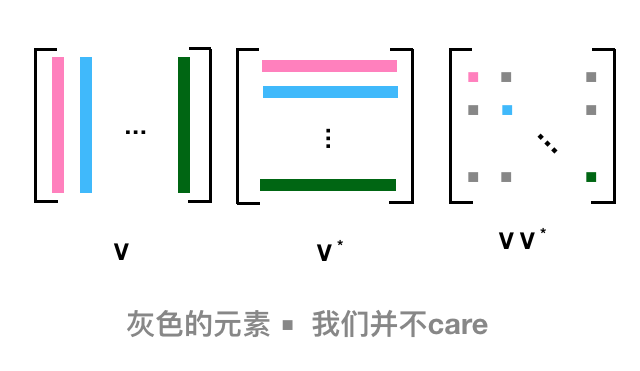
\includegraphics{images/Frobenius.png}

至于 \(tr(AB) = tr(BA)\) 也是可以跟上面一样的看法 \(Tr(AB) = Tr (BA) = \sum a_{ij} b_{ji}\), 这个结论也可以推广:

\begin{itemize}
\tightlist
\item
  \({\displaystyle \operatorname {tr} (\mathbf {A} \mathbf {B} \mathbf {C} )=\operatorname {tr} \left(\left(\mathbf {A} \mathbf {B} \mathbf {C} \right)^{\mathsf {T}}\right)=\operatorname {tr} (\mathbf {C} \mathbf {B} \mathbf {A} )=\operatorname {tr} (\mathbf {A} \mathbf {C} \mathbf {B} ),}\)
\item
  \({\displaystyle \operatorname {tr} (\mathbf {A} \mathbf {B} \mathbf {C} \mathbf {D} )=\operatorname {tr} (\mathbf {B} \mathbf {C} \mathbf {D} \mathbf {A} )=\operatorname {tr} (\mathbf {C} \mathbf {D} \mathbf {A} \mathbf {B} )=\operatorname {tr} (\mathbf {D} \mathbf {A} \mathbf {B} \mathbf {C} )}\) , ABCD 呈循环状
\end{itemize}

最小化 \(-2tr(Y^T R X)\) 也就是最大化 \(tr(Y^T R X)\)

\[
\begin{aligned}
tr(Y^TRX)  {}
&= tr(RXY^T) & tr(AB) = tr(BA) \\
&= tr(R U \Sigma V^T) & XY^T = U \Sigma V^T \\ 
&= tr(\Sigma V^T R U ) & tr(AB) = tr(BA) \\ 
&= tr(\Sigma M) & M = V^TRU, \text{also orthogonal} \\
&= \sum_i \sigma_im_{ii} & \Sigma \text{ is diagonal}
\end{aligned}  
\]

\(M = V^TRU\) 正交矩阵的乘积依旧正交,很好证明:

\[
AA^T = A^TA =  I \\
BB^T = B^TB = I \\
(AB)^T(AB) = B^TA^TAB = B^TB = I
\]

更一般,上面这个 \(M = V^TRU\) = \(V^T (RU)\), 所以当然也是正交矩阵。

最后这里是这样的:

\[
tr(\Sigma M) = \begin{bmatrix} \sigma_1 &  &  & &  \\  & \sigma_2 &  &  \\  &  &  & \ddots &  \\ &   &  &  & \sigma_n\end{bmatrix} \begin{bmatrix} m_{11} & m_{12} &  \dots  & m_{1d} \\ m_{21} &  m_{22} & \dots  & m_{2d}  \\ \vdots & \vdots & \vdots  & \vdots \\ m_{d1} &  m_{d2} & \dots  & m_{dd}  \end{bmatrix}  = \sum_{i=1}^d\sigma_im_{ii} \le \sum_{i=1}^d \sigma_i
\]

M 作为正交阵,满足:

\[
1 = m_j^Tm_j = \sum_{i=1}^d m_{ij}^2 \implies m_{ij}^2 \le 1 \implies |m_{ij}| \le 1
\]

M 是正交阵, 所以 \(m_ii \le 1\), 奇异值分解,所以 \(\sigma_i \ge 0\), 所以我们会想要尝试去 M 对角线上的最大值,也就是当 M = I 的时候,代入回去可以知道:

\[
I = M = V^TRU \implies V = RU \implies R = VU^T
\]

这个问题又被称为:Procrustes Problem

\begin{quote}
普洛克路斯忒斯(希腊语:Προκρούστης)也称达玛斯蒂斯(希腊语:Δαμαστής)是希腊神话中的一名强盗。他是海神波塞冬的儿子,在从雅典到埃莱夫西纳的路上开设黑店,拦截行人。店内设有一张铁床,旅客投宿时,将身高者截断,身矮者则强行拉长,使与床的长短相等。而由于普洛克路斯忒斯秘密地拥有两张长度不同的床,所以无人能因身高恰好与床相等而幸免。后来英雄忒修斯前往雅典时,路过此地,将其杀死。
\end{quote}

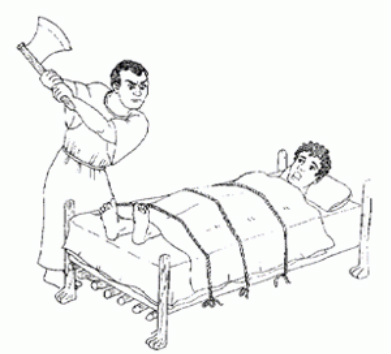
\includegraphics{images/Procrustes.jpg}

这个问题的叫法和来源有点意思嘛。

\textbf{最小化 \(\parallel X - RY \parallel ^2\) 的正交矩阵 R 满足: \(R = VU^T\), 其中 \(XY^T = U \Sigma V^T\)}

具体求解我们一般可能是这么来操作的:

\begin{enumerate}
\def\labelenumi{\arabic{enumi}.}
\tightlist
\item
  固定 R, 针对 t 最小化 E
\item
  固定 t, 针对 R 最小化 E (R 需要满足 \(R^TR = I\))
\item
  再回到第一步
\end{enumerate}

这样直到收敛。

\hypertarget{apar}{%
\section{APAR}\label{apar}}

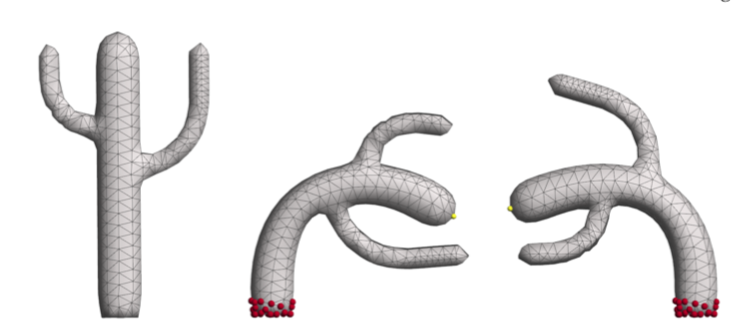
\includegraphics{images/APAR_01.png}

有一篇著名的 paper, As-Rigid-As-Possible Surface Modeling,用的就是 key idea 就是对齐、 SVD 分解 以及上面的迭代求解。

\hypertarget{pca}{%
\section{PCA}\label{pca}}

PCA 之前也写过,包括特别具体的步骤:

\begin{itemize}
\tightlist
\item
  算出质心 : \(m = \frac{1}{n} \sum_{i=1}^n x_i\)
\item
  去中心化: \(y_i = x_i - m\)
\item
  散布/协方差矩阵 : \(S = YY^T\) 其中 Y 的列为 \(y_i\)
\item
  特征分解 : \(S = V \Lambda V^T\)
\item
  特征值排序 : \(\lambda_1 \ge \lambda_2 \ge \cdots \ge \lambda_d\)
\item
  特征向量排序 : \(v_1, \cdots, v_d\)
\item
  取出我们需要的部分
\end{itemize}

\hypertarget{ux56feux50cfux538bux7f29}{%
\section{图像压缩}\label{ux56feux50cfux538bux7f29}}

还记的之前的文章\href{https://zhuanlan.zhihu.com/p/114550672}{奇异值分解}中写到了 Eckart-Yound Theorem(低维矩阵近似):

\begin{quote}
我们想找到一个找到一个 rank 为 r 的矩阵 \(\tilde{A}\) 来近似 A, 做法就是将 A 进行 SVD 分解, \(A = U \Sigma V^T\) , 然后我们取其中前 r 个 最大的奇异值,重组 \(\tilde{A} = U \Sigma_r V^T\) , 这样的重组会使得 \(\parallel \tilde{A} - A \parallel_{Fro}\) 最小化。
\end{quote}

\[
\Sigma_r = \begin{bmatrix} \sigma_1 & &  & &  \\  & \ddots  &  &  \\  &  & \sigma_r & & \\  &  &  & 0 & \\ &   &  &  & \ddots \\ &   &  & & & 0 \end{bmatrix} 
\]

这里我们来看一个具体的例子,假设我先读入一幅图片,这幅图片是 RGBA 的,矩阵的维度是 m x n x 4, 这样处理的话有点麻烦,我先把它转成灰色的, 这样矩阵就是 m x n, 处理起来比较简单。 (m x n x 4 应该也可以通过类似的方法来处理)。

对灰色的图像,我们做 SVD 分解,然后我们再抽出 前10个、前20个、前50个 最大的奇异值来重新组成图片,看结果:

\begin{Shaded}
\begin{Highlighting}[]
\ImportTok{import}\NormalTok{ numpy }\ImportTok{as}\NormalTok{ np}
\ImportTok{import}\NormalTok{ matplotlib.pyplot }\ImportTok{as}\NormalTok{ plt}
\ImportTok{import}\NormalTok{ matplotlib.image }\ImportTok{as}\NormalTok{ mpimg}

\KeywordTok{def}\NormalTok{ rgb2gray(rgb):}
    \ControlFlowTok{return}\NormalTok{ np.dot(rgb[...,:}\DecValTok{3}\NormalTok{], [}\FloatTok{0.299}\NormalTok{, }\FloatTok{0.587}\NormalTok{, }\FloatTok{0.144}\NormalTok{])}

\NormalTok{img }\OperatorTok{=}\NormalTok{ mpimg.imread(}\StringTok{\textquotesingle{}Mona\_Lisa.png\textquotesingle{}}\NormalTok{)}
\NormalTok{gray }\OperatorTok{=}\NormalTok{ rgb2gray(img)}
\NormalTok{plt.imshow(gray, cmap }\OperatorTok{=}\NormalTok{ plt.get\_cmap(}\StringTok{\textquotesingle{}gray\textquotesingle{}}\NormalTok{))}

\NormalTok{U, s, Vh }\OperatorTok{=}\NormalTok{ np.linalg.svd(gray)}

\KeywordTok{def}\NormalTok{ composite(U, s, Vh, n):}
    \ControlFlowTok{return}\NormalTok{ np.dot(U[:, :n], np.dot(np.diag(s[:n]), Vh[:n,:]))}

\ControlFlowTok{for}\NormalTok{ i }\KeywordTok{in}\NormalTok{ [}\DecValTok{10}\NormalTok{, }\DecValTok{20}\NormalTok{, }\DecValTok{50}\NormalTok{]:}
\NormalTok{    new\_img }\OperatorTok{=}\NormalTok{ composite(U, s, Vh, i)}
\NormalTok{    plt.imshow(new\_img, cmap}\OperatorTok{=}\StringTok{\textquotesingle{}gray\textquotesingle{}}\NormalTok{)}
\NormalTok{    title }\OperatorTok{=} \StringTok{"new\_img\_}\SpecialCharTok{\%s}\StringTok{"} \OperatorTok{\%}\NormalTok{ i}
\NormalTok{    plt.title(title)}
\NormalTok{    plt.savefig(title }\OperatorTok{+} \StringTok{\textquotesingle{}.png\textquotesingle{}}\NormalTok{)}
\NormalTok{    plt.show()}
\end{Highlighting}
\end{Shaded}

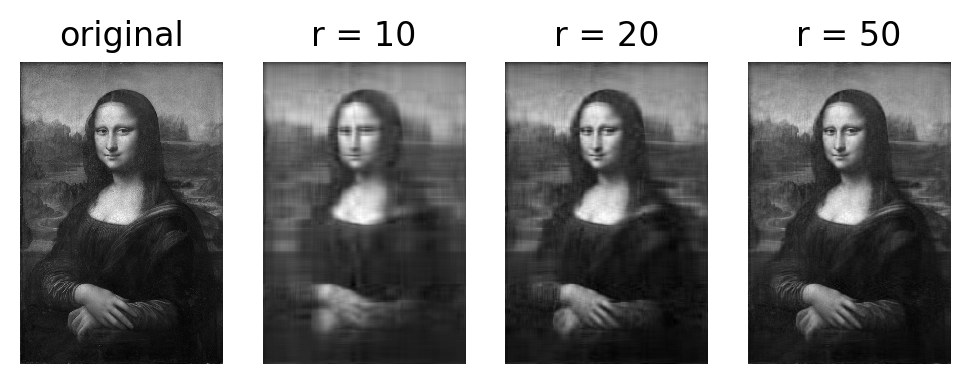
\includegraphics{images/final.png}

有点意思。

我觉得一种更 简单/感性 的理解方式是:

\begin{quote}
对称阵特征向量分解的基础是谱分析,而奇异值分解则是谱分析理论在任意矩阵上的推广。
\end{quote}

就是把这个看成一种分解、然后近似重建的方式,可以说类似 傅里叶分析,我们可以取一定的频率来重建原本的信号。

或者更感性的理解可以是这样,比如我们有空间的任意一个\((x, y, z)^T\)向量,如果我们只想要xy平面上的向量来模拟它,当然取 \((x, y)^T\) ,降低了维度,但是我们还是想尽量在靠近这个向量。

或者又像那么多我们学过的展开,比如一个多项式:

\[f(x) = a_n x^n + a_{n-1} x^{n-a} + \cdots + a_1 x + a_0\]

我们可以取 \(a_n \cdots, a_r\) 来模拟这个 \(f(x)\) ,虽然不是全等,但已经足够靠近。o(╯□╰)o

\hypertarget{ux77e9ux9635ux5206ux89e3-matirx-application}{%
\chapter{矩阵分解 \{matirx application\}}\label{ux77e9ux9635ux5206ux89e3-matirx-application}}

总结一下之前我们碰到的矩阵的各种分解方式,在开始之前先补充一些定义。

\hypertarget{ux5b9aux4e49-1}{%
\section{定义}\label{ux5b9aux4e49-1}}

\hypertarget{ux5171ux8f6dux8f6cux7f6e-conjugate-transpose}{%
\subsection{共轭转置 Conjugate transpose}\label{ux5171ux8f6dux8f6cux7f6e-conjugate-transpose}}

如果我们有一个复数矩阵A:

\[
{\displaystyle {\boldsymbol {A}}={\begin{bmatrix}1&-2-i&5\\1+i&i&4-2i\end{bmatrix}}}
\]

它的转置\(A^T\):

\[{\displaystyle {\boldsymbol {A}}^{\mathrm {T} }={\begin{bmatrix}1&1+i\\-2-i&i\\5&4-2i\end{bmatrix}}}\]

共轭转置\(\overline{A^T}\):

\[{\displaystyle \overline{{\boldsymbol {{A}}}^{\mathrm {T}} }={\begin{bmatrix}1&1-i\\-2+i&-i\\5&4+2i\end{bmatrix}}}\]

共轭转置也经常记为: \(A^*, A^H(这个写法跟下面的 Hermitian 定义有关), \overline{A^T}\)

\hypertarget{hermitian}{%
\subsection{Hermitian}\label{hermitian}}

Hermitian matrix 埃尔米特矩阵: 埃尔米特矩阵中每一个第i行第j列的元素都与第j行第i列的元素的复共轭。 也就是这个矩阵等于它的共轭转置。

复数我们知道 \(z = a + ib \in \mathbb{C}\), 共轭我们也清楚 \(\bar{z} = a - ib\)

\[
{\displaystyle A{\text{ Hermitian}}\quad \iff \quad a_{ij}={\overline {a_{ji}}}} \\
{\displaystyle A{\text{ Hermitian}}\quad \iff \quad A=A^{\mathsf {H}}}
\]

如果 \(A \in \mathbb{R}^{n \times n}\) 是实数矩阵,并且是 Hermitian, 那么 \(a_{ij} = a_{ji}\), 这就是一个对称矩阵。一般来说,实对称矩阵我们一般就说它是实对称矩阵,不过我们知道,它也是 Hermitian。

如果我们有一个复数矩阵A,那么它需要等于它的共轭转置, 比如:

\[
{\displaystyle A = {\begin{bmatrix}2&2+i&4\\2-i&3&i\\4&-i&1\\\end{bmatrix}}}
\]

其实 Hermitian 也暗示了我们这个矩阵需要是方阵,至少我们转置之后的维度要跟原来的相等嘛。

\hypertarget{ux6b63ux5b9a-positive-definite}{%
\subsection{正定 positive definite}\label{ux6b63ux5b9a-positive-definite}}

一个 n × n 的实对称矩阵 M 是正定的,当且仅当对于所有的非零实系数向量z,都有 \(z^TMz > 0\) 。其中 \(z^T\) 表示 z 的转置。

\[
{\displaystyle M{\text{ positive definite}}\quad \iff \quad x^{\textsf {T}}Mx>0{\text{ for all }}x\in \mathbb {R} ^{n}\setminus \mathbf {0} }
\]

首先 实对称矩阵 M 并不一定正定的, 比如 M = -I :

\[
\begin{bmatrix}1 & 0 & 1\end{bmatrix}\begin{bmatrix}-1 & 0 & 0 \\ 0 & -1 & 0 \\ 0 & 0 & -1 \end{bmatrix}\begin{bmatrix}1 \\ 0 \\ 1\end{bmatrix} = -2 < 0
\]

对于复数,一个 n×n 的埃尔米特矩阵 M是正定的当且仅当对于每个非零的复向量z,都有\(z^*Mz > 0\)。其中z*表示z的共轭转置。由于 M是埃尔米特矩阵,经计算可知,对于任意的复向量z,\(z^*Mz\)必然是实数,从而可以与0比较大小。因此这个定义是自洽的。

\[{\displaystyle M{\text{ positive definite}}\quad \iff \quad x^{*}Mx>0{\text{ for all }}x\in \mathbb {C} ^{n}\setminus \mathbf {0} }
\]

Hermitian 也当然不一定正定,我们可以有一些判定方法:

\begin{itemize}
\tightlist
\item
  矩阵M的所有的特征值 \(\lambda_i\) 都是正的
\item
  \ldots{}
\end{itemize}

\hypertarget{ux6b63ux4ea4ux77e9ux9635-orthogonal-matrix}{%
\subsection{正交矩阵 orthogonal matrix}\label{ux6b63ux4ea4ux77e9ux9635-orthogonal-matrix}}

\[Q^{T}=Q^{-1}\Leftrightarrow Q^{T}Q=QQ^{T}=I.\,\!\]

\[{\displaystyle 1=det(I)=det(Q^{T}Q)=det(Q^{T})det(Q)=(det(Q))^{2}\Rightarrow det(Q)=\pm 1}\]

\begin{itemize}
\tightlist
\item
  作为一个线性映射(变换矩阵),正交矩阵保持距离不变,所以它是一个保距映射,具体例子为旋转与镜射。
\item
  行列式值为+1的正交矩阵,称为特殊正交矩阵(special orthogonal group),它是一个旋转矩阵。
\item
  行列式值为-1的正交矩阵,称为瑕旋转矩阵。瑕旋转是旋转加上镜射。镜射也是一种瑕旋转。
\item
  所有 n × n 的正交矩阵形成一个群 O(n),称为正交群。亦即,正交矩阵与正交矩阵的乘积也是一个正交矩阵。
\item
  所有特殊正交矩阵形成一个子群SO(n),称为特殊正交群。亦即,旋转矩阵与旋转矩阵的乘积也是一个旋转矩阵。
\end{itemize}

\hypertarget{ux9149ux77e9ux9635-unitary-matrix}{%
\subsection{酉矩阵 unitary matrix}\label{ux9149ux77e9ux9635-unitary-matrix}}

酉矩阵/幺正矩阵:

\[{\displaystyle U^{*}U=UU^{*}=I_{n}}\]

就是 U 和其 共轭转置 \(U^*\) 乘积为 单位矩阵。它是 正交矩阵 在复数上的推广。

\begin{quote}
酉(汉语拼音:yǒu)为地支的第十位,其前为申、其后为戌。酉月为农历八月,酉时为二十四小时制的17:00至19:00,在方向上指正西方。五行里酉代表金,阴阳学说里酉为阴。
\end{quote}

说实话,这个字之前还没注意过它怎么念。unitary 作为 unit 的形容词,单位的、一元的,鉴于单位矩阵这个已经被 take 了,被翻成 幺正矩阵 也和不错,也大概有一元那么个意思。翻成酉矩阵大概也是文化人才能做到吧。

酉矩阵有很多很好的性质:

\begin{itemize}
\tightlist
\item
  \({\displaystyle U^{-1}=U^{*}}\), 酉矩阵必定可逆,且逆矩阵等于其共轭转置:
\item
  \(|\lambda_n| = 1\), 酉矩阵 U 的所有特征值 \(λ_n\) ,其绝对值都是等于 1 的复数:
\item
  \({\displaystyle \left|\det(U)\right|=1}\), 酉矩阵 U 行列式的绝对值也是 1
\item
  \({\displaystyle (U\vec {x} )\cdot (U\vec {y} )=\vec {x} \cdot \vec {y} }\), 酉矩阵 U 不会改变两个复向量
  \(\vec{x}\) 和 \(\vec{y}\) 的点积
\item
  \ldots{}
\end{itemize}

\hypertarget{ux6b63ux89c4ux77e9ux9635-normal-matrix}{%
\subsection{正规矩阵 normal matrix}\label{ux6b63ux89c4ux77e9ux9635-normal-matrix}}

正规矩阵(英语:normal matrix)A 是与自己的共轭转置满足交换律的复系数方块矩阵,也就是说,A 满足
\[\mathbf{A}^* \mathbf{A} =  \mathbf{A} \mathbf{A}^*\]

\(A^*\) 是 A 的共轭转置。

如果 A是实系数矩阵,则 \(A^* = A^T\),从而条件简化为 \(AA^T = A^TA\).

正规矩阵的概念十分重要,因为它们正是能使谱定理成立的对象:矩阵 A 正规当且仅当它可以被成 \(A = U \Lambda U^*\) 的形式。其中的\(\Lambda = diag(\lambda_1, \lambda_2, \dots)\)为对角矩阵,U 为酉矩阵。

总而言之,就是 正规矩阵 一定可以 特征分解/频谱分解/谱定理。

\hypertarget{ux7c7bux6bd4}{%
\subsection{类比}\label{ux7c7bux6bd4}}

不同种类的正规矩阵可以与各种复数建立对应的类比关系。比如:

\begin{itemize}
\tightlist
\item
  可逆矩阵类似于非零的复数。
\item
  矩阵的共轭转置类似于复数的共轭
\item
  酉矩阵类似于模等于1的复数。
\item
  埃尔米特矩阵类似于实数。
\item
  埃尔米特矩阵中的正定矩阵类似于正实数。
\end{itemize}

\hypertarget{ux5206ux89e3}{%
\section{分解}\label{ux5206ux89e3}}

\hypertarget{a-plu}{%
\subsection{A = PLU}\label{a-plu}}

\begin{itemize}
\tightlist
\item
  适用:方阵
\item
  分解: A = PLU, L 是 下三角阵, U 是 上三角阵,而 P 则是 permutation 行变换,单位矩阵变换可得, 如果没有行变换,A 就 直接分解成 LU. PLU 分解源自高斯消元法。
\end{itemize}

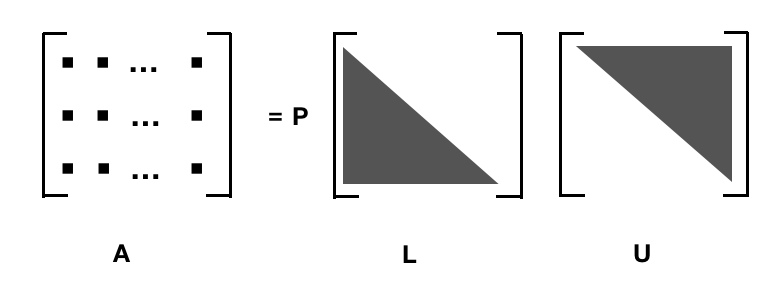
\includegraphics{images/Gauss_03_APLU.png}

所有的方阵都可以写成 PLU 分解的形式。

\hypertarget{cholesky-ux5206ux89e3}{%
\subsection{Cholesky 分解}\label{cholesky-ux5206ux89e3}}

\begin{itemize}
\tightlist
\item
  适用:方阵、hermitian、正定 positive definite
\item
  分解: \(A = LL^*\)
\end{itemize}

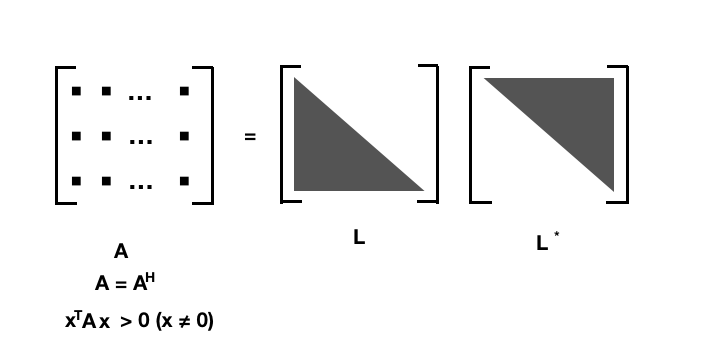
\includegraphics{images/Cholesky.png}

A 是正定的 Hermitian阵, L 是下三角矩阵, \(L^*\) 是 L 的共轭转置, 是一个上三角.

\hypertarget{qrux5206ux89e3}{%
\subsection{QR分解}\label{qrux5206ux89e3}}

\begin{itemize}
\tightlist
\item
  适用于: 列向量线性无关的矩阵 m x n, m ≥ n
\item
  分解:A = QR, Q 是 m x m 的 酉矩阵, 又叫做幺正矩阵(unitary matrix), R 是一个上三角矩阵
\end{itemize}

对于方阵的 QR 分解我比较熟悉

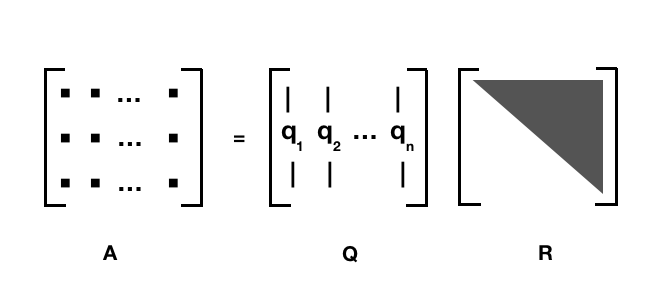
\includegraphics{images/AQR.png}

如果A不是方阵的话,那么三角矩阵只会占据一部分,下面会都是0, 所以经常也这样写 QR 分解:

\[{\displaystyle A=QR=Q{\begin{bmatrix}R_{1}\\0\end{bmatrix}}={\begin{bmatrix}Q_{1},Q_{2}\end{bmatrix}}{\begin{bmatrix}R_{1}\\0\end{bmatrix}}=Q_{1}R_{1}}\]

\begin{quote}
where R1 is an n×n upper triangular matrix, 0 is an (m − n)×n zero matrix, Q1 is m×n, Q2 is m×(m − n), and Q1 and Q2 both have orthogonal columns.
\end{quote}

计算 QR 分解 我们可以用 Gram--Schmidt 或者 Householder reflections.

\hypertarget{ux7279ux5f81ux5206ux89e3ux9891ux8c31ux5206ux89e3-eigendecomposition-spectral-decomposition}{%
\subsection{特征分解/频谱分解 Eigendecomposition / spectral decomposition}\label{ux7279ux5f81ux5206ux89e3ux9891ux8c31ux5206ux89e3-eigendecomposition-spectral-decomposition}}

\begin{itemize}
\tightlist
\item
  适用于: 具有线性独立特征向量(不一定是不同特征值)的方阵 A
\item
  分解:\(\mathbf{A}=\mathbf{Q}\mathbf{\Lambda}\mathbf{Q}^{-1}\)
\end{itemize}

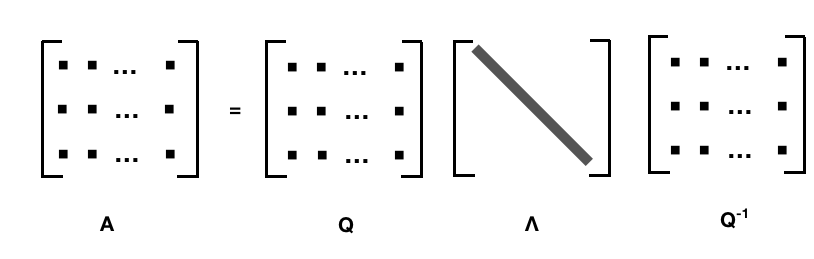
\includegraphics{images/eigen_00.png}

Q 是 n x n 的矩阵, 第 i 列是 A 的 特征向量 \(\vec{q}_i\), \(\Lambda\) 是对角阵,其中第 i个 对角元素\(\Lambda_{ii} = \lambda_i\), 是跟 特征向量 \(\vec{q}_i\) 对应的 特征值 \(\lambda_i\). 这里需要注意只有可对角化矩阵才可以作特征分解。比如\({\displaystyle {\begin{bmatrix}1&1\\0&1\\\end{bmatrix}}}\) 不能被对角化,也就不能特征分解。

一般来说,特征向量 \(\vec{q}_i, ( i = 1, \cdots, N)\) 一般被单位化(但这不是必须的)。未被单位化的特征向量组 \(\vec{q}_i, ( i = 1, \cdots, N)\) 也可以作为 Q 的列向量。这一事实可以这样理解: Q 中向量的长度都被 \(Q^{-1}\) 抵消了。

这里我们虽然用了 Q 这个字母,但是我们并没有说它是一个正交阵,因为之前写特征分解的时候也提到过:

\begin{quote}
对于任意矩阵,其对应于不同特征值的特征向量线性无关,但不一定正交,而对于实对称矩阵,其对应于不同特征值的特征向量是相互正交的。
\end{quote}

特征分解很容易推导:

\[
{\displaystyle {\begin{aligned}\mathbf {A} \mathbf {v} &=\lambda \mathbf {v} \\\mathbf {A} \mathbf {Q} &=\mathbf {Q} \mathbf {\Lambda } \\\mathbf {A} &=\mathbf {Q} \mathbf {\Lambda } \mathbf {Q} ^{-1}.\end{aligned}}}
\]

\begin{itemize}
\tightlist
\item
  实对称矩阵
\end{itemize}

对于任意的 n x n 实对称矩阵都有 n 个线性无关的特征向量,并且这些特征向量都可以正交单位化而得到一组正交且模为 1 的向量。所以:

\[\mathbf{A}=\mathbf{Q}\mathbf{\Lambda}\mathbf{Q}^{T}  \]

其中 Q 为正交矩阵, \(\Lambda\) 为对角矩阵。

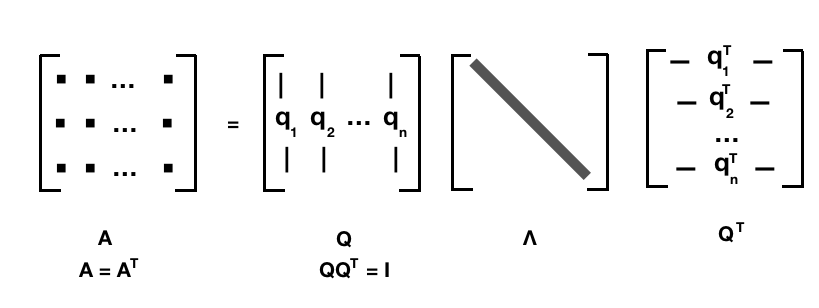
\includegraphics{images/eigen_01.png}

\begin{itemize}
\tightlist
\item
  正规矩阵
\end{itemize}

一个复正规矩阵具有一组正交特征向量基,故正规矩阵可以被分解成
\[\mathbf{A}=\mathbf{U}\mathbf{\Lambda}\mathbf{U}^{*}  \]

其中 U 是 酉矩阵。

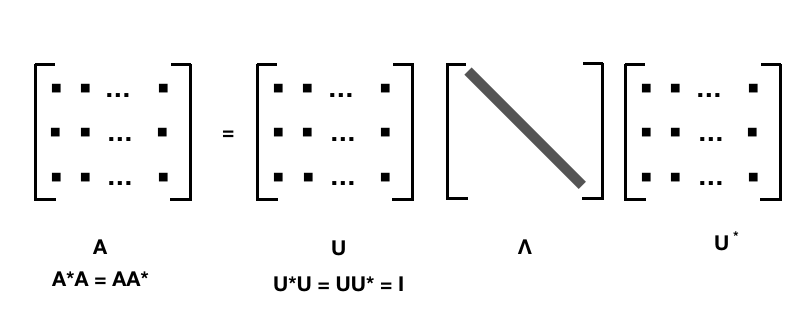
\includegraphics{images/eigen_02.png}

\begin{quote}
特征分解对于理解线性常微分方程或线性差分方程组的解很有用。 例如,差分方程 \(x_{t+1} = A x_t\) 从初始条件开始 \(x_0 = c\) 到 \(x_{t}=A^{t}c\) ,相当于 \$x\_\{t\}=VD\textsuperscript{\{t\}V}\{\{-1\}\}c \$,其中V和D是由A的特征向量和特征值形成的矩阵。 由于D是对角线,D 的 t 次幂 \$ D\^{}\{t\}\$ 只是涉及将对角线上的每个元素的 t 次幂 。 这与 A 的 t的次幂相比 ,更容易实现和理解,因为A通常不是对角线。
\end{quote}

这里就直接点出了一个 特征分解的应用场景。 解 线性常微分方程 或 线性差分方程组。

\hypertarget{ux5947ux5f02ux503cux5206ux89e3}{%
\subsection{奇异值分解}\label{ux5947ux5f02ux503cux5206ux89e3}}

\begin{itemize}
\tightlist
\item
  适用于: m x n 矩阵A
\item
  分解: \(A=U \Sigma V^*\), U 和 V 都是 酉矩阵/幺正矩阵, 也就是满足 \(U^*U= V^*V = I\), \(\Sigma\) 是对角阵,对角上的元素称为A的奇异值 ,
\item
  U 和 V 并不一定是唯一的。
\end{itemize}

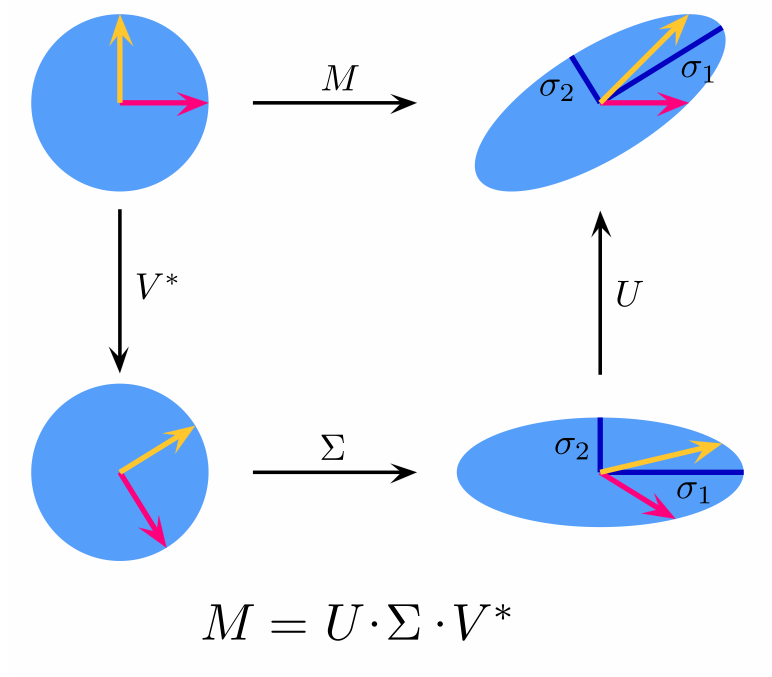
\includegraphics{images/svd_headline.png}

至此,线性/矩阵相关暂时告一段落。

\begin{center}\rule{0.5\linewidth}{0.5pt}\end{center}

Matlab/numpy 都内置了这些分解方式,而对我们来说,重要的是在合适的场景中选择合适的工具来解决问题。

参考:
大量参考 wikipedia

\hypertarget{ux975eux7ebfux6027ux65b9ux7a0bux6c42ux89e3-nonlinear-equation}{%
\chapter{非线性方程求解 \{nonlinear equation\}}\label{ux975eux7ebfux6027ux65b9ux7a0bux6c42ux89e3-nonlinear-equation}}

我们从求根开始,对于非线性方程,可能 set up 是这样的:

\[
f: \mathbb{R}^n \to \mathbb{R}^m \\
\vec{x}^* :  f(\vec{x}^* ) = \vec{0}
\]

我们先考虑最简单的情况: \(f : \mathbb{R} \to \mathbb{R}\)

首先,我们可能会有很多奇奇怪怪的函数,首先,我们需要对函数做一些假设:

\begin{itemize}
\tightlist
\item
  连续: \(x \to y, f(x) \to f(y)\)
\item
  Lipschitz 连续: \(| f(x) - f(y) | \le C |x - y|\)
\item
  可微: \(\forall x, \exists f'(x)\)
\item
  \(C^k\) : k阶可微,连续, 记得古典微分几何研究的大部分 \(C^\infty\)
\end{itemize}

\hypertarget{ux4e8cux5206ux6cd5-bisection-method}{%
\section{二分法 Bisection method}\label{ux4e8cux5206ux6cd5-bisection-method}}

中间值定理:

\begin{quote}
假设有一连续函数 \(f:[a,b]\mapsto \mathbb {R}\),且假设 f(a) \textless{} f(b),若对任意数 u 满足 f(a) \textless{} u \textless{} f(b),则存在一点 c, a \textless{} c \textless{} b,使得 f(c)=u,当 f(a) \textgreater{} f(b) 时也有类似叙述。
\end{quote}

直观地比喻,这代表在{[}a,b{]}区间上可以画出一个连续曲线,而不让笔离开纸面。

若要求已知函数 f(x) = 0 的根 (x 的解),则:

\begin{enumerate}
\def\labelenumi{\arabic{enumi}.}
\tightlist
\item
  先找出一个区间 {[}a, b{]},使得f(a)与f(b)异号。根据中间值定理,这个区间内一定包含着方程式的根。
\item
  求该区间的中点 \(m={\frac {a+b}{2}}\),并找出 f(m) 的值。
\item
  f(m) = 0, 返回 m
\item
  若 f(m) 与 f(a) 正负号相同则取 {[}m, b{]} 为新的区间, 否则取 {[}a, m{]}.
\item
  重复第2和第3步至理想精确度为止。
\end{enumerate}

这个算法还是很容易理解。并且它一定会 work, 它的收敛速度是线性的。

\hypertarget{ux4e0dux52a8ux70b9-fixed-point}{%
\section{不动点 fixed point}\label{ux4e0dux52a8ux70b9-fixed-point}}

fixed point 满足:

\[
g(x) = x
\]

如果我们想求不动点,令:

\[
x_0 \\
x_{k+1} = g(x_k)
\]

这样迭代我们就可以求到不动点。

如果我们令

\[
g(x) = f(x) + x 
\]

然后找到 g(x) 的不动点那么也就是找到了 f(x) 的根。

如果收敛的话,经常是二次收敛,所以速度优于二分法。

\hypertarget{ux725bux987fux6cd5-newtons-method}{%
\section{牛顿法 Newton's method}\label{ux725bux987fux6cd5-newtons-method}}

牛顿法很出名:

\[
x_{k+1} = x_k - \frac{f(x_k)}{f'(x_k)}
\]

牛顿法的优点同样是二次收敛,缺点是 f'(x) 可能会难求,o(╯□╰)o

\hypertarget{ux5272ux7ebfux6cd5-secant-method}{%
\section{割线法 Secant method}\label{ux5272ux7ebfux6cd5-secant-method}}

f'(x) 难求所以有割线法:

\[
x_{k+1} = x_k - \frac{f(x_k)(x_k - x_{k-1})}{f(x_k) - f(x_{k-1})}
\]

感觉这个就是用 数值来代替 f'(x), 不过割线需要两个初始值 \(x_0, x_1\), 割线法的收敛速度率是 \({\displaystyle \alpha ={\frac {1+{\sqrt {5}}}{2}}\approx 1.618}\)

这些方法当然也可以混起来用。

\hypertarget{ux8ba1ux7b97-5}{%
\section{计算}\label{ux8ba1ux7b97-5}}

如果我想求解:

\[
\cos(x) - x^3 = 0
\]

使用 numpy :

\begin{Shaded}
\begin{Highlighting}[]
\ImportTok{import}\NormalTok{ numpy }\ImportTok{as}\NormalTok{ np}
\ImportTok{from}\NormalTok{ scipy.optimize }\ImportTok{import}\NormalTok{ fsolve}

\KeywordTok{def}\NormalTok{ func(x):}
    \ControlFlowTok{return}\NormalTok{ np.cos(x) }\OperatorTok{{-}}\NormalTok{ x}\OperatorTok{**}\DecValTok{3}

\NormalTok{result }\OperatorTok{=}\NormalTok{ fsolve(func, }\DecValTok{1}\NormalTok{)}
\BuiltInTok{print}\NormalTok{(result)}
\CommentTok{\# 0.86547403}
\BuiltInTok{print}\NormalTok{( func(result) )}
\CommentTok{\#2.22044605e{-}16}
\end{Highlighting}
\end{Shaded}

x = 0.86547 也算精度ok的解了。

\hypertarget{ux975eux7ebfux6027ux65b9ux7a0bux7ec4ux6c42ux89e3-nonlinear-equations}{%
\chapter{非线性方程组求解 \{nonlinear equations\}}\label{ux975eux7ebfux6027ux65b9ux7a0bux7ec4ux6c42ux89e3-nonlinear-equations}}

继续讨论

\[
f: \mathbb{R}^n \to \mathbb{R}^m \\
\vec{x}^* :  f(\vec{x}^* ) = \vec{0}
\]

我们一般会认为 n ≥ m. \(f(\vec{x}) = A \vec{x} - \vec{b}\) 当然是属于上面讨论过的一种我们已经知道怎么处理的情况。

\hypertarget{ux725bux987fux6cd5}{%
\section{牛顿法}\label{ux725bux987fux6cd5}}

\hypertarget{ux96c5ux53efux6bd4ux77e9ux9635-jacobian-matrix}{%
\subsection{雅可比矩阵 Jacobian matrix}\label{ux96c5ux53efux6bd4ux77e9ux9635-jacobian-matrix}}

\[
(Df)_{ij} = \frac{\partial f_i}{\partial x_j} =  {\begin{bmatrix}{\dfrac {\partial \mathbf {f} }{\partial x_{1}}}&\cdots &{\dfrac {\partial \mathbf {f} }{\partial x_{n}}}\end{bmatrix}} 
= {\begin{bmatrix}{\dfrac {\partial f_{1}}{\partial x_{1}}}&\cdots &{\dfrac {\partial f_{1}}{\partial x_{n}}}\\\vdots &\ddots &\vdots \\{\dfrac {\partial f_{m}}{\partial x_{1}}}&\cdots &{\dfrac {\partial f_{m}}{\partial x_{n}}}\end{bmatrix}}
\]

\begin{quote}
如果函数 \(f: \mathbb{R}^n \to \mathbb{R}^m\) 在点 x 可微的话,在点 x 的雅可比矩阵即为该函数在该点的最佳线性逼近,也代表雅可比矩阵是单变数实数函数的微分在向量值多变数函数的推广,在这种情况下,雅可比矩阵也被称作函数 f 在点 x 的微分或者导数。
\end{quote}

\[
f(\vec{x}) \approx f(\vec{x}_k) + Df(\vec{x}_k)(\vec{x} - \vec{x}_k)
\]

所以我们可以在非线性方程组上推广牛顿法:

\[
\vec{x}_{k+1} = \vec{x}_k - [Df(\vec{x}_k)]^{-1} f(\vec{x}_k)
\]

我们可以令:

\[
[Df(\vec{x}_k)]^{-1} f(\vec{x}_k) = \vec{y}_k
\]

所以:

\[
[Df(\vec{x}_k)] \vec{y}_k = f(\vec{x}_k)
\]

这样可以避免直接求 \([Df(\vec{x}_k)]^{-1}\), 可以用高斯消元法求出 \(\vec{y}_k\).

牛顿法的收敛条件为:雅克比矩阵特征值的最大模小于1,此时收敛速度为二次。

使用牛顿法的缺点依旧是:

\begin{itemize}
\tightlist
\item
  微分比较难
\item
  雅克比矩阵 \(Df(\vec{x}_k)\) 每次都会变化,增大计算量
\end{itemize}

\hypertarget{broydens-method}{%
\section{Broyden's method}\label{broydens-method}}

Broyden's method 是一种拟牛顿法,还是以牛顿法为基础,注意割线法中我们用数值来代替 f'(x):

\[
f'(x_{k}) \approx {\frac {f(x_{k})-f(x_{k-1})}{x_{k}-x_{k-1}}} \\
x_{k+1}=x_{k}-{\frac {f(x_{k})}{f'(x_{k})}}
\]

这里我们的想法也是类似的:

\[
J \cdot ( \vec{x}_{k} - \vec{x}_{k-1})  \approx   f(\vec{x}_{k}) - f(\vec{x}_{k-1})  \\
J \approx Df(\vec{x}_k)
\]

\begin{itemize}
\tightlist
\item
  保持\(\vec{x}_k\) 和 \(J_k\)
\item
  用类似牛顿法更新 \(\vec{x}_k\)
\item
  用类似割线法更新 \(J_k\)
\end{itemize}

更具体来说就是:

\[
 \text{minimize}_{J_k} \parallel J_k - J_{k-1} \parallel_{Fro} ^2 \\
 \text{such that  } J \cdot ( \vec{x}_{k} - \vec{x}_{k-1})  \approx   f(\vec{x}_{k}) - f(\vec{x}_{k-1}) 
\]

在满足上述条件的情况下,我们可以用拉格朗日乘子法推导出:

\[
J_k= J_{k-1}+{\frac { ( f(\vec{x}_k) - f(\vec{x}_{k-1}) - J_{k-1}\Delta \vec{x} ) }{\|\vec{x}_k - \vec{x}_{k-1} \|^{2}}} (\Delta \vec{x}^T)  \\
\vec{x}_{k+1} = \vec{x}_k - J_k^{-1} f(\vec{x}_k)
\]

我们可以初始化 \(J_0 = I\), 不过我们依旧需要计算\(J_k^{-1}\), 注意观察:

\[
J_k= J_{k-1}+{\frac { ( f(\vec{x}_k) - f(\vec{x}_{k-1}) - J_{k-1}\Delta \vec{x} ) }{\|\vec{x}_k - \vec{x}_{k-1} \|^{2}}} (\Delta \vec{x}^T)
\]

我们可以把它写成:

\[
J_k= J_{k-1}+ \vec{u}_k\vec{v}_k^T
\]

利用 Sherman-Morrison Formula:

\[
{\displaystyle \left(A+uv^{\textsf {T}}\right)^{-1}=A^{-1}-{A^{-1}uv^{\textsf {T}}A^{-1} \over 1+v^{\textsf {T}}A^{-1}u}.}
\]

可以推导出:

\[
J_k^{-1} = J_{k-1}^{-1} - \frac{ J_{k-1}^{-1} \vec{u}_k \vec{v}_k^T J_{k-1}^{-1}  }{ 1 + \vec{v}_k^T J_{k-1}^{-1} \vec{u}_k}
\]

所以用上面这个式子来计算 \(J_k^{-1}\).

\hypertarget{ux8ba1ux7b97-6}{%
\section{计算}\label{ux8ba1ux7b97-6}}

我们依旧可以用 scipy 中的 fsolve 来尝试计算:

\[
\begin{cases}
 x_0 + x_1^2 = 4 \\
 e^{x_0} + {x_0}{x_1} = 3\\
\end{cases}
\]

\begin{Shaded}
\begin{Highlighting}[]
\ImportTok{from}\NormalTok{ scipy.optimize }\ImportTok{import}\NormalTok{ fsolve}
\ImportTok{import}\NormalTok{ math}

\KeywordTok{def}\NormalTok{ equations(p):}
\NormalTok{    x0, x1 }\OperatorTok{=}\NormalTok{ p}
    \ControlFlowTok{return}\NormalTok{ ( x0 }\OperatorTok{+}\NormalTok{ x1}\OperatorTok{**}\DecValTok{2} \OperatorTok{{-}} \DecValTok{4}\NormalTok{, math.exp(x0) }\OperatorTok{+}\NormalTok{ x0 }\OperatorTok{*}\NormalTok{ x1 }\OperatorTok{{-}}\DecValTok{3}\NormalTok{ )}

\NormalTok{x0, x1 }\OperatorTok{=}\NormalTok{ fsolve(equations, (}\DecValTok{1}\NormalTok{, }\DecValTok{1}\NormalTok{))}

\BuiltInTok{print}\NormalTok{(x0, x1)}
\CommentTok{\# 0.6203445234801195 1.8383839306750887}
\BuiltInTok{print}\NormalTok{(equations((x0, x1)))}
\CommentTok{\# (4.4508396968012676e{-}11, {-}1.0512035686360832e{-}11)}
\end{Highlighting}
\end{Shaded}

\hypertarget{ux4e34ux754cux70b9ux9a7bux70b9ux62d0ux70b9ux978dux70b9ux9876ux70b9ux66f2ux7ebf-points-concepts}{%
\chapter{临界点、驻点、拐点、鞍点、顶点(曲线) \{Points Concepts\}}\label{ux4e34ux754cux70b9ux9a7bux70b9ux62d0ux70b9ux978dux70b9ux9876ux70b9ux66f2ux7ebf-points-concepts}}

\hypertarget{ux4e34ux754cux70b9-critial-point}{%
\section{临界点 critial point}\label{ux4e34ux754cux70b9-critial-point}}

\begin{itemize}
\tightlist
\item
  \(f: \mathbb{R} \to \mathbb{R}\): 不可微或者导数为0的点
\item
  \(f: \mathbb {C} \to \mathbb{C}\): 不是全纯(?)或者导数等于0
\item
  \(f: \mathbb {R}^n \to \mathbb{R}\): 梯度没有定义或者等于0
\item
  \(f: \mathbb {R}^m \to \mathbb{R}^n\): Jacobian的秩 不是最大的
\end{itemize}

临界点是我们用来求极值可能出现的点。

\hypertarget{ux9a7bux70b9-stationary-point}{%
\section{驻点 stationary point}\label{ux9a7bux70b9-stationary-point}}

驻点(stationary point) 是指的 \(f: \mathbb{R} \to \mathbb{R}\) 情况下的临界点,看驻点的定义:

\[
 \left.\frac{dy}{dx}\right|_p=0 \,
\]

之所以翻译成 驻点(stationary point) 我想应该是正因为这一点导数为0, 微小的 x 变化并不带来 y 的变化,所以叫 stationary point,翻译成驻点也合理。

\hypertarget{ux62d0ux70b9-inflection-point}{%
\section{拐点 inflection point}\label{ux62d0ux70b9-inflection-point}}

inflect 本身就有弯曲、改变的意思。

最近大家都在讲的`拐点',英文也可以是 inflection、 flex。

\begin{quote}
拐点(Inflection point)或称反曲点,是一条连续曲线改变凹凸性的点,或者等价地说,是使切线穿越曲线的点。
\end{quote}

说起来这个 convex 和 concave 也是有一点令人窒息的:

\hypertarget{convex-ux51f8ux51fdux6570}{%
\subsection{convex 凸函数}\label{convex-ux51f8ux51fdux6570}}

\[{\displaystyle f((1-\alpha )x+\alpha y)\leq (1-\alpha )f(x)+\alpha f(y)}\]

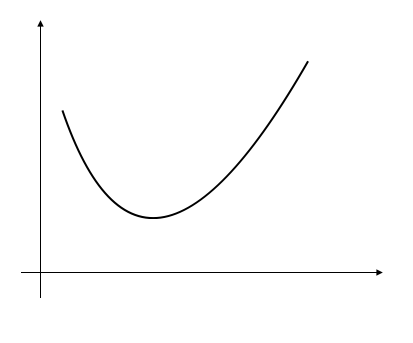
\includegraphics{images/ConvexDef.png}

\hypertarget{concave-ux51f9ux51fdux6570}{%
\subsection{concave 凹函数:}\label{concave-ux51f9ux51fdux6570}}

\[{\displaystyle f((1-\alpha )x+\alpha y)\geq (1-\alpha )f(x)+\alpha f(y)}\]

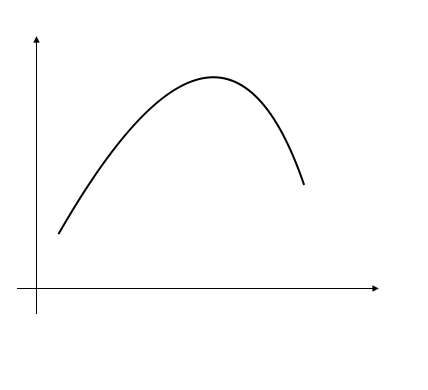
\includegraphics{images/ConcaveDef.png}

我要窒息了,我还是学别人来这样记吧, convex v , concave/cave 洞穴

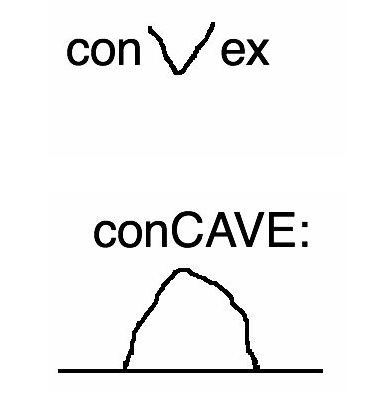
\includegraphics{images/convex_concave.png}

或者我来记 convex下凸, concave上凸

红色的点是 驻点/临界点 stationary points/critial points, 蓝色的点是 拐点 inflection points.

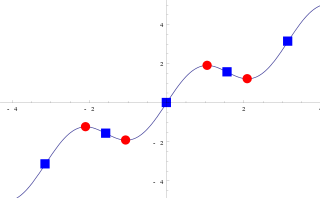
\includegraphics{images/320px-Stationary_vs_inflection_pts.png}

inflection point :

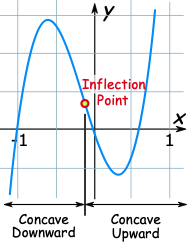
\includegraphics{images/5x3-2x2-3x-concave.png}

拐点并不是不连续,毕竟满足了曲线的定义都 \(C^0\) 连续, 上面这个曲线是 正弦曲线,是一个\(C^\infty\) 连续的。它只是一种 convex/concave 的变化。

\hypertarget{ux978dux70b9-saddle-point}{%
\section{鞍点 saddle point}\label{ux978dux70b9-saddle-point}}

\begin{quote}
一个不是局部极值点的驻点称为鞍点。
\end{quote}

鞍点的英文是 saddle point 或者 minmax point.

鞍点来自于双曲面,比如下图 \(f(x,y) = x^2 - y^2\), 在(0, 0) 是一个临界点,但它并不是极值点,长得像马鞍的形状,所以叫鞍点。

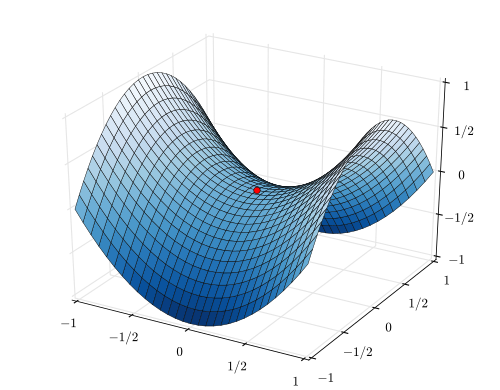
\includegraphics{images/Saddle_point.png}

\begin{quote}
在一维空间里,鞍点是驻点·也是拐点。因为函数图形在鞍点由凸转凹,或由凹转凸。
\end{quote}

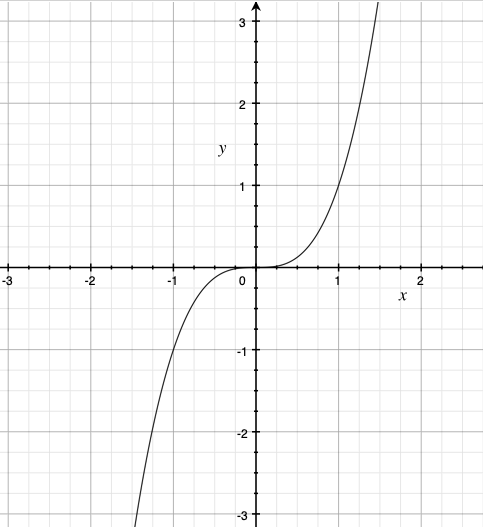
\includegraphics{images/y_cubic_x.png}

比如 \$y = x\^{}3 \$ 在 (0, 0) 处即是驻点也是拐点。

\hypertarget{ux9876ux70b9ux66f2ux7ebfvertex-curve}{%
\section{顶点(曲线)vertex (curve)}\label{ux9876ux70b9ux66f2ux7ebfvertex-curve}}

强调这个顶点是属于曲线的

\begin{quote}
在平面曲线中, 顶点是曲率的一阶导数为零的点。 这通常是曲率的局部最大值或最小值,并且一些人将顶点定义为更具体地是曲率的局部极限点。
\end{quote}

考虑抛物线 \(y = ax^2 + bx + c\)

它的有符号的曲率是:

\[{\displaystyle k(x)={\frac {2a}{\left(1+(2ax+b)^{2}\right)^{\frac {3}{2}}}}.}\]

它的曲率极值点在 \(x = -b/2a\) 处取到,这个点是它的驻点(导数也为0),同时这个点也是它的顶点。

\hypertarget{ux5bfcux6570ux68afux5ea6-jacobianhessian-gradient-related-concepts}{%
\chapter{导数、梯度、 Jacobian、Hessian \{Gradient Related Concepts\}}\label{ux5bfcux6570ux68afux5ea6-jacobianhessian-gradient-related-concepts}}

之前写过关于\href{https://zhuanlan.zhihu.com/p/97545154}{梯度}的文章,是从线性近似着手开始写起,这里我再次回顾梯度和一些相关的矩阵:

\begin{itemize}
\tightlist
\item
  一元函数: \(f: \mathbb{R} \to \mathbb{R}\)
\item
  多元函数: \(f: \mathbb{R}^n \to \mathbb{R}\)
\item
  向量函数: \(f: \mathbb{R}^n \to \mathbb{R}^m\)
\end{itemize}

以下讨论都预先预设假设 f 必定可导甚至更高阶可导。

\hypertarget{ux5bfcux6570}{%
\section{导数}\label{ux5bfcux6570}}

针对一元函数 \(f: \mathbb{R} \to \mathbb{R}\), 近似:

\[f(x) \approx f(x_0) + f'(x_0)(x-x_0)\]

\hypertarget{ux68afux5ea6}{%
\section{梯度}\label{ux68afux5ea6}}

梯度针对多元函数 \(f: \mathbb{R}^n \to \mathbb{R}\) ,是导数的推广, 它的结果是一个向量:

\[
\nabla f = \begin{pmatrix} \frac{\partial f}{\partial x_1} \\ \frac{\partial f}{\partial x_2} \\ \vdots \\ \frac{\partial f}{\partial x_n}  \end{pmatrix}
\]

也经常写为, 函数相对于 n x 1 向量 \(\vec{x}\) 的梯度算子为 \(\nabla_{\boldsymbol{x}}\):

\[
\nabla_{\boldsymbol{x}} \overset{\underset{\mathrm{def}}{}}{=} \left[ \frac{\partial }{\partial x_1}, \frac{\partial }{\partial x_2},\cdots,\frac{\partial }{\partial x_n} \right]^T=\frac{\partial }{\partial \boldsymbol{x}}
\]

近似:

\[f(\vec{x}) \approx f(\vec{x}_0) + \nabla f(\vec{x}_0) \cdot (\vec{x} - \vec{x}_0)\]

\hypertarget{jacobian-ux96c5ux53efux6bd4ux77e9ux9635}{%
\section{Jacobian 雅可比矩阵}\label{jacobian-ux96c5ux53efux6bd4ux77e9ux9635}}

我喜欢 Jacobian 的英文读音,听起来很可爱。

针对向量函数 \(f: \mathbb{R}^n \to \mathbb{R}^m\)

\begin{quote}
如果函数 \(f: \mathbb{R}^n \to \mathbb{R}^m\) 在点 x 可微的话,在点 x 的雅可比矩阵即为该函数在该点的最佳线性逼近,也代表雅可比矩阵是单变数实数函数的微分在向量值多变数函数的推广,在这种情况下,雅可比矩阵也被称作函数 f 在点 x 的微分或者导数。
\end{quote}

\[
{\displaystyle \mathbf {J} ={\begin{bmatrix}{\dfrac {\partial \mathbf {f} }{\partial x_{1}}}&\cdots &{\dfrac {\partial \mathbf {f} }{\partial x_{n}}}\end{bmatrix}}={\begin{bmatrix}{\dfrac {\partial f_{1}}{\partial x_{1}}}&\cdots &{\dfrac {\partial f_{1}}{\partial x_{n}}}\\\vdots &\ddots &\vdots \\{\dfrac {\partial f_{m}}{\partial x_{1}}}&\cdots &{\dfrac {\partial f_{m}}{\partial x_{n}}}\end{bmatrix}}}
\]

矩阵分量:

\[
{\displaystyle \mathbf {J} _{ij}={\frac {\partial f_{i}}{\partial x_{j}}}.}
\]

其它常用符号:

\({\displaystyle Df}、 {\displaystyle \mathrm {D} \mathbf {f} }、{\displaystyle \mathbf {J} _{\mathbf {f} }(x_{1},\ldots ,x_{n})}\) 或者 \({\displaystyle {\frac {\partial (f_{1},\ldots ,f_{m})}{\partial (x_{1},\ldots ,x_{n})}}.}\)

近似:

\[
f(\vec{x}) \approx f(\vec{x}_k) + J(\vec{x}_k)(\vec{x} - \vec{x}_k)
\]

如果 m = n,那么 Jacobian 可以形成方阵,这个矩阵可以计算出它的行列式:

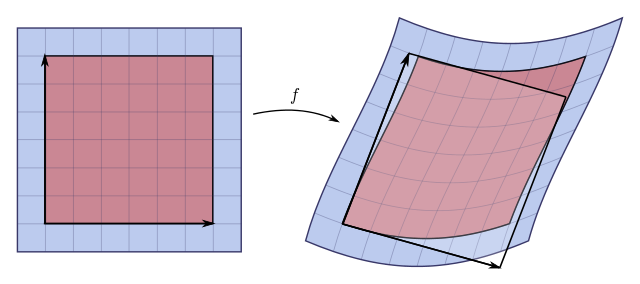
\includegraphics{images/640px-Jacobian_determinant_and_distortion.png}

叫做 Jacobian Matrix,它的意义是比如这个微小形状改变的比值。

\hypertarget{hessian-ux9ed1ux585eux77e9ux9635}{%
\section{Hessian 黑塞矩阵}\label{hessian-ux9ed1ux585eux77e9ux9635}}

适用于 \(f: \mathbb{R}^n \to \mathbb{R}\) 有点二阶导数的意思:

\[
{\displaystyle \mathbf {H} ={\begin{bmatrix}{\frac {\partial ^{2}f}{\partial x_{1}^{2}}}&{\frac {\partial ^{2}f}{\partial x_{1}\,\partial x_{2}}}&\cdots &{\frac {\partial ^{2}f}{\partial x_{1}\,\partial x_{n}}}\\\\{\frac {\partial ^{2}f}{\partial x_{2}\,\partial x_{1}}}&{\frac {\partial ^{2}f}{\partial x_{2}^{2}}}&\cdots &{\frac {\partial ^{2}f}{\partial x_{2}\,\partial x_{n}}}\\\\\vdots &\vdots &\ddots &\vdots \\\\{\frac {\partial ^{2}f}{\partial x_{n}\,\partial x_{1}}}&{\frac {\partial ^{2}f}{\partial x_{n}\,\partial x_{2}}}&\cdots &{\frac {\partial ^{2}f}{\partial x_{n}^{2}}}\end{bmatrix}}\,}
\]

是一个 n x n 的方阵,也可以写成:

\[
{\displaystyle \mathbf {H} _{ij}={\frac {\partial ^{2}f}{\partial x_{i}\partial x_{j}}}}
\]

之所以说它二次导数,看一下它的推导 :

\begin{itemize}
\tightlist
\item
  \(f: \mathbb{R} \to \mathbb{R}\)
\end{itemize}

\[
f(x) \approx f(x_0) + f'(x_0 )(x − x_0 ) + \frac{1}{2}f''(x_0 )(x − x_0 )^2
\]

\begin{itemize}
\tightlist
\item
  \(f: \mathbb{R}^n \to \mathbb{R}\):
\end{itemize}

\[
f(x_1,x_2)=f(x_{10},x_{20})+f_{x_1}(x_{10},x_{20})\Delta x_1+f_{x_2}(x_{10},x_{20})\Delta x_2+\frac {1}{2}[f_{x_1 x_1}(x_{10},x_{20})\Delta x_1^2+2f_{x_1 x_2}(x_{10},x_{20})\Delta x_1\Delta x_2+f_{x_2 x_2}(x_{10},x_{20})\Delta x_2^2]
\]

其中 \({\displaystyle \Delta x_{1}=x_{1}-x_{10}\,},{\displaystyle \Delta x_{2}=x_{2}-x_{20}\,},{\displaystyle f_{x_{1}}={\frac {\partial f}{\partial x_{1}}}\,},{\displaystyle f_{x_{2}}={\frac {\partial f}{\partial x_{2}}}\,},{\displaystyle f_{x_{1}x_{1}}={\frac {\partial ^{2}f}{\partial x_{1}^{2}}}\,},{\displaystyle f_{x_{2}x_{2}}={\frac {\partial ^{2}f}{\partial x_{2}^{2}}}\,},{\displaystyle f_{x_{1}x_{2}}={\frac {\partial ^{2}f}{\partial x_{1}\partial x_{2}}}={\frac {\partial ^{2}f}{\partial x_{2}\partial x_{1}}}\,}\)

写成向量形式:

\[f(\vec{x}) \approx f(\vec{x_0}) +   \nabla f(\vec{x_0}) \cdot (\vec{x} - \vec{x_0}) + \frac{1}{2}(\vec{x} - \vec{x_0})^TH(\vec{x_0})(\vec{x} - \vec{x_0})\]

其中

\[
{\displaystyle H(x_{0})={\begin{bmatrix}{\frac {\partial ^{2}f}{\partial x_{1}^{2}}}&{\frac {\partial ^{2}f}{\partial x_{1}\,\partial x_{2}}}\\\\{\frac {\partial ^{2}f}{\partial x_{2}\,\partial x_{1}}}&{\frac {\partial ^{2}f}{\partial x_{2}^{2}}}\end{bmatrix}}_{x_{0}}\,}
\]

所以推广到更高阶就如上所示,那么Hessian 的一个很具体的应用就是,判断函数的极值,正如导数的作用一样。

一元函数: \(f: \mathbb{R} \to \mathbb{R}\) ,在 \$ x=x\_0\$ 点处具有二阶导数,且 \(f'(x_{0})=0, f''(x_{0}) \neq 0\), 则

\begin{itemize}
\tightlist
\item
  \(f''(x) < 0\), 极大值
\item
  \(f''(x) > 0\), 极小值
\item
  \(f''(x) = 0\), 鞍点
\item
  \(f''(x)\) 不存在,没法直接判断,或许是极值点
\end{itemize}

那么针对于 \(f: \mathbb{R}^n \to \mathbb{R}\), 在 \(\vec{x}_0\) 处梯度为 \(\vec{0}\),那么我们可以用 \(H(\vec{x_0})\) 来帮助判断:

\begin{itemize}
\tightlist
\item
  H 正定, 极小值
\item
  H 负定, 极大值
\item
  H 不定, 鞍点
\item
  H 不可逆, 也不能直接判断
\end{itemize}

至于判定矩阵是否正定可以:

\begin{itemize}
\tightlist
\item
  尝试Cholesky分解,看其是否存在
\item
  计算所有的特征值,看是否为正
\end{itemize}

\hypertarget{ux65e0ux7ea6ux675fux4f18ux5316-optimization-without-constraintss}{%
\chapter{无约束优化 \{Optimization without constraintss\}}\label{ux65e0ux7ea6ux675fux4f18ux5316-optimization-without-constraintss}}

\hypertarget{ux4f8bux5b50-1}{%
\section{例子}\label{ux4f8bux5b50-1}}

之前我们讨论了许多优化问题:

\begin{longtable}[]{@{}lll@{}}
\toprule
\begin{minipage}[b]{0.30\columnwidth}\raggedright
问题\strut
\end{minipage} & \begin{minipage}[b]{0.30\columnwidth}\raggedright
目标函数\strut
\end{minipage} & \begin{minipage}[b]{0.30\columnwidth}\raggedright
约束\strut
\end{minipage}\tabularnewline
\midrule
\endhead
\begin{minipage}[t]{0.30\columnwidth}\raggedright
最小二乘法\strut
\end{minipage} & \begin{minipage}[t]{0.30\columnwidth}\raggedright
\(E(\vec{x}) = \parallel A\vec{x} - \vec{b} \parallel^2\)\strut
\end{minipage} & \begin{minipage}[t]{0.30\columnwidth}\raggedright
无\strut
\end{minipage}\tabularnewline
\begin{minipage}[t]{0.30\columnwidth}\raggedright
把\(\vec{b}\) 投影到 \(\vec{a}\) 上\strut
\end{minipage} & \begin{minipage}[t]{0.30\columnwidth}\raggedright
\(E(c) = \parallel c\vec{a} - \vec{b} \parallel^2\)\strut
\end{minipage} & \begin{minipage}[t]{0.30\columnwidth}\raggedright
无\strut
\end{minipage}\tabularnewline
\begin{minipage}[t]{0.30\columnwidth}\raggedright
实对称矩阵的特征向量\strut
\end{minipage} & \begin{minipage}[t]{0.30\columnwidth}\raggedright
\(E(\vec{x}) = \vec{x}^TA\vec{x}\)\strut
\end{minipage} & \begin{minipage}[t]{0.30\columnwidth}\raggedright
\(\parallel \vec{x} \parallel = 1\)\strut
\end{minipage}\tabularnewline
\begin{minipage}[t]{0.30\columnwidth}\raggedright
Pseudoinverse\strut
\end{minipage} & \begin{minipage}[t]{0.30\columnwidth}\raggedright
\(E(\vec{x}) = \parallel \vec{x} \parallel^2\)\strut
\end{minipage} & \begin{minipage}[t]{0.30\columnwidth}\raggedright
\(A^TA\vec{x} = A^T\vec{b}\)\strut
\end{minipage}\tabularnewline
\begin{minipage}[t]{0.30\columnwidth}\raggedright
主成分分析\strut
\end{minipage} & \begin{minipage}[t]{0.30\columnwidth}\raggedright
\(E(C) = \parallel X - CC^TX \parallel_{Fro}\)\strut
\end{minipage} & \begin{minipage}[t]{0.30\columnwidth}\raggedright
\(C^TC = I_{d \times d}\)\strut
\end{minipage}\tabularnewline
\begin{minipage}[t]{0.30\columnwidth}\raggedright
Broyden step\strut
\end{minipage} & \begin{minipage}[t]{0.30\columnwidth}\raggedright
\(E(J_k) = \parallel J_k - J_{k-1} \parallel_{Fro}^2\)\strut
\end{minipage} & \begin{minipage}[t]{0.30\columnwidth}\raggedright
\(J_k \cdot (\vec{x}_k - \vec{x}_{k-1}) = f(\vec{x}_k) - f(\vec{x}_{k-1})\)\strut
\end{minipage}\tabularnewline
\bottomrule
\end{longtable}

有些是有约束的,有些没有,我们现在先考虑无约束的问题,set up 如下:

\[
min_{\vec{x}} f(\vec{x})
\]

\begin{itemize}
\tightlist
\item
  例子一
\end{itemize}

可以有很多例子,比如数据拟合,类似最小二乘法,不过现在我们是想用一个指数来拟合:

\[
E(a, c) = \sum_i (y_i - c e^{ax_i})^2
\]

\begin{itemize}
\tightlist
\item
  例子二
\end{itemize}

给一堆数据,怀疑正态分布,用正态分布来拟合:

\[
g(h; \mu, \sigma)={\frac {1}{\sigma {\sqrt {2\pi }}}}e^{-(h - \mu)^2/2 \sigma^2}
\]

给一大堆独立数据 \({h_1, \cdots, h_n}\) :

\[
P({h_1, \cdots, h_n}; \mu, \sigma) = \prod_i g(h_i, \mu, \sigma)
\]

要求估算出 \(\mu, \sigma\) 来最大化概率分布, 感觉 贝叶斯/NLP 中间会有很多这种模型的应用。

\begin{itemize}
\tightlist
\item
  例子三
\end{itemize}

给一堆数据,我们想找到它的几何中心(geometric median),注意这个不同于质心,比如下图:

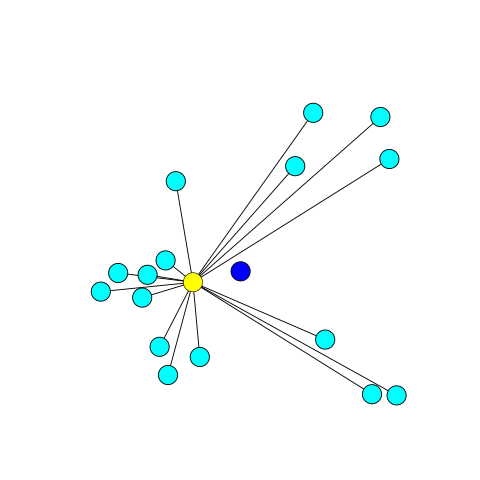
\includegraphics{images/480px-Geometric_median_example.png}

蓝色的店是质心,黄色的点是几何中心,几何中心满足:

\[
E(\vec{x}) = \sum_i \parallel \vec{x} - \vec{x}_i \parallel_2
\]

注意这里只是 l2 norm, 并没有平方。

\hypertarget{ux6781ux503c}{%
\section{极值}\label{ux6781ux503c}}

全局最小值:

\[
\vec{x}^* \in  \mathbb{R}^n \\
f: \mathbb{R}^n \to \mathbb{R} \\
\forall \vec{x} \in \mathbb{R}^n f(\vec{x})^* \le f(\vec{x}) 
\]

局部最小值:

\[
\vec{x}^* \in  \mathbb{R}^n \\
f: \mathbb{R}^n \to \mathbb{R} \\
\forall \parallel \vec{x} - \vec{x}^* \parallel < \varepsilon,   f(\vec{x})^* \le f(\vec{x}) 
\]

最大值的定义也是类似的,无约束优化其实就是一个求极值的问题。求极值这个问题我们在数学上还是比较熟悉的。同样,我们从一元函数开始。

\hypertarget{ux4e00ux5143ux51fdux6570}{%
\section{一元函数}\label{ux4e00ux5143ux51fdux6570}}

\hypertarget{ux725bux987fux6cd5-1}{%
\subsection{牛顿法}\label{ux725bux987fux6cd5-1}}

\(f: \mathbb{R} \to \mathbb{R}\), 如果函数可微,那么极值的可能出现点就包括了 驻点、边界以及导数不存在的点,此处我们集中讨论驻点的情况。也就是导数 \(f'(x) = 0\) 的点 。 鉴于之前我们已经讨论过一元函数求根 \(f(x) = 0\)。 这里无非也就是变成了求解 \(f'(x) = 0\), 那么依旧可以使用 牛顿法:

\[
{\displaystyle x_{k+1} = x_{k}-{\frac {f'(x_{k})}{f''(x_{k})}}.}
\]

\hypertarget{ux9ec4ux91d1ux5206ux5272ux641cux7d22-golden-section-search}{%
\subsection{黄金分割搜索 Golden-section search}\label{ux9ec4ux91d1ux5206ux5272ux641cux7d22-golden-section-search}}

适用条件: 单峰函数 Unimodal function, 顾名思义 单峰 unimodular 就是指的有一个峰值。

单峰:

\begin{figure}
\centering
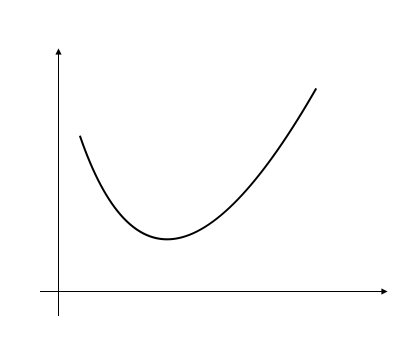
\includegraphics{images/unimodular.png}
\caption{unimodular.png}
\end{figure}

双峰:

\begin{figure}
\centering
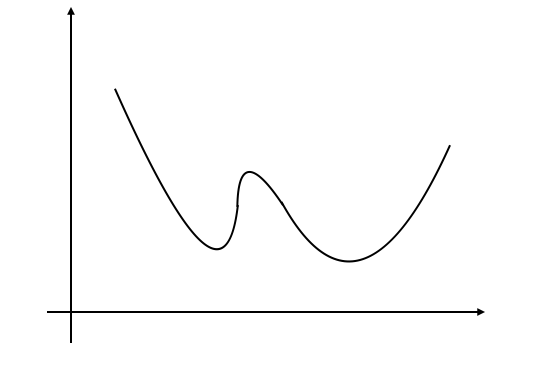
\includegraphics{images/Bimodal.png}
\caption{Bimodal.png}
\end{figure}

单峰定义:
\(f: [a, b] \to \mathbb{R}\) 存在 \(x^* \in [a, b]\) 满足 f 在 \(x \in [a, x^*]\) 是递减, 在 \(x \in [x^*, b]\) 递增。

我们可以利用单峰的性质来用之前类似二分的思路求解。

\begin{figure}
\centering
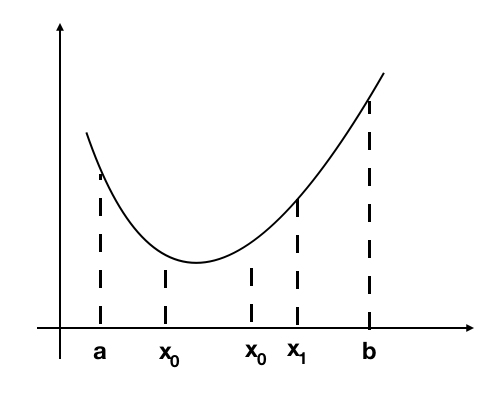
\includegraphics{images/unimodal_01.png}
\caption{unimodal\_01.png}
\end{figure}

假设 \(a < x_0 < x_1 < b\), 假设我们有:

\begin{itemize}
\tightlist
\item
  \(f(x_0) \le f(x_1)\) , 那么对于 \(x \in [x_1, b]\), 都有 \(f(x) \ge f(x_0)\), 最小值点 \(x^* \in [a, x_1]\), 所以可以丢掉区间 \([x_1, b]\)
\item
  \(f(x_0) \ge f(x_1)\) , 那么对于 \(x \in [a, x_0]\), 都有 \(f(x) \ge f(x_1)\), 最小值点 \(x^* \in [x_0, b]\), 所以可以丢掉区间 \([a, x_0]\)
\end{itemize}

但是这样每一轮需要计算 \(f(x_0), f(x_1)\), 懒的本性想让我们重复利用之前的计算结果,所以我们这样来考虑,假设 a = 0, b = 1, 第一轮我们计算:

\[x_0 = \alpha, x_1 = 1 - \alpha, \alpha \in (0, \frac{1}{2})\]

\begin{itemize}
\tightlist
\item
  假设是上面的 \(f(x_0) \le f(x_1)\) 的情况的话,区间变成:
\end{itemize}

\[[a, x_1] = [0, 1- \alpha]\]

第二轮我们的选择点是:

\[\alpha(1- \alpha), (1 - \alpha)^2\]

如果

\[x_0 = \alpha = (1 - \alpha)^2 \]

那么 我们就可以减少一次计算:

\[\alpha^2 - 3 \alpha + 1 = 0 \\
\alpha = \frac{1}{2}(3 - \sqrt{5}) \\
1 - \alpha = \frac{1}{2}(\sqrt{5} - 1) \]

\(1 - \alpha = \tau\) 满足黄金分割比例。

\begin{itemize}
\tightlist
\item
  假设是上面的 \(f(x_0) \ge f(x_1)\) 的状况, 区间变成:
\end{itemize}

\[
[x_0, 1] = [\alpha, 1]
\]

第二轮选择点是:

\[\alpha + \alpha(1- \alpha), \alpha + (1 - \alpha)^2\]

如果:

\[x_0 = 1 - \alpha = \alpha + \alpha(1 - \alpha) \]

得到相同的方程式,相同的解,所以我们可以有 黄金分割搜索:

\begin{enumerate}
\def\labelenumi{\arabic{enumi}.}
\tightlist
\item
  初始化 a, b 使得 f 在 {[}a, b{]} 上是 unimodular
\item
  \(x_0 = a + (1-\tau)(b-a), x_1 = a + \tau(b-a), f_0 = f(x_0), f_1 = f(x_1)\)
\item
  迭代直到 b - a 足够小:

  \begin{itemize}
  \tightlist
  \item
    \(f_0 \ge f_1\), 丢掉 \([a, x_0]\)

    \begin{itemize}
    \tightlist
    \item
      \(a \gets x_0\)
    \item
      \(x_0 \gets x_1, f_0 \gets f_1\)
    \item
      \(x_1 \gets a + \tau(b-a), f_1 \gets f(x_1)\)
    \end{itemize}
  \item
    \(f_1 > f_0\), 丢掉 \([x_1, b]\)

    \begin{itemize}
    \tightlist
    \item
      \(b \gets x_1\)
    \item
      \(x_1 \gets x_0, f_1 \gets f_0\)
    \item
      \(x_0 \gets a + (1-\tau)(b-a), f_0 \gets f(x_0)\)
    \end{itemize}
  \end{itemize}
\end{enumerate}

\hypertarget{ux591aux5143ux51fdux6570}{%
\section{多元函数}\label{ux591aux5143ux51fdux6570}}

\(f: \mathbb{R}^n \to \mathbb{R}\), 针对多元函数,感觉最出名就是梯度下降了(类比下山)。

\hypertarget{ux68afux5ea6ux4e0bux964dux6cd5}{%
\subsection{梯度下降法}\label{ux68afux5ea6ux4e0bux964dux6cd5}}

\begin{quote}
梯度下降方法基于以下的观察:如果实值函数 \(F(\vec{x})\) 在点 \(\vec {a}\) 处可微且有定义,那么函数 \(F(\vec{x})\) 在 \(\vec{a}\) 点沿着梯度相反的方向 \(-\nabla F({\vec {a}})\) 下降最多。
\end{quote}

\begin{quote}
因而,如果 \({\vec {b}}={\vec {a}}-\gamma \nabla F({\vec {a}})\) 对于 \$ \gamma \textgreater0\$ 为一个够小数值时成立,那么 \(F({\vec {a}})\geq F({\vec {b}})\)。
\end{quote}

所以我们可以有梯度下降法的明确步骤:

\begin{itemize}
\tightlist
\item
  随机预估的 \(x_0\)
\item
  \(g_k(t) = f(\vec{x}_k - t \nabla f(\vec{x}_k))\)
\item
  搜索找到 \(t^* \ge 0\) 同时最小化 \(g_k\)
\item
  \(\vec{x}_{k+1} = \vec{x}_k - t^* \nabla f(\vec{x}_k)\)
\end{itemize}

\hypertarget{ux725bux987fux6cd5-2}{%
\subsection{牛顿法}\label{ux725bux987fux6cd5-2}}

同样类似一元函数,我们可以推广牛顿法:

\[\vec{x}_{k+1} = \vec{x}_k - [H_f(\vec{x}_k)]^{-1} \nabla f(\vec{x}_k)\]

使用牛顿法的问题在于 \(\nabla f(\vec{x})\) 已经比较难计算了,而再加上 Hessian 矩阵,痛苦+n, 所以我们依旧寻求之前的 单变量 拟牛顿法 Quasi-Newton method 来前进。

\hypertarget{bfgs}{%
\subsection{BFGS}\label{bfgs}}

想不到 BFGS 的全称是 Broyden--Fletcher--Goldfarb--Shanno algorithm,此 Shanno 非彼 Shanno,是四位研究优化的数学家的名字,这个算法类似之前出现过的 Broyden's method, 我们用矩阵来近似Hessian 矩阵 :

\[
\vec{x}_{k+1} = \vec{x}_k - \alpha_k B_{k}^{-1}\nabla f(\vec{x}_k) \\
B_k \approx H_f(\vec{x}_k)
\]

\[
B_{k+1} ( \vec{x}_{k+1} - \vec{x}_k)  =  \nabla f(\vec{x}_{k+1}) - \nabla f(\vec{x}_{k}) 
\]

B 有一些很好的性质:

\begin{itemize}
\tightlist
\item
  对称
\item
  半正定
\end{itemize}

所以我们需要做的优化就是:

\[
min_{B_{k+1}} \parallel B_{k+1} - B_k \parallel \\
s.t. B_{k+1}^T = B_{k+1} \\
B_{k+1} ( \vec{x}_{k+1} - \vec{x}_k)  =  \nabla f(\vec{x}_{k+1}) - \nabla f(\vec{x}_{k}) 
\]

而 \$\parallel B\_\{k+1\} - B\_k \parallel  \$ 最小化 并不能保证 \$\parallel B\_\{k+1\}\^{}\{-1\} - B\_k\^{}\{-1\} \parallel \$ 很小,所以我们应当要求解的是:

\[
min_{H_{k+1}} \parallel H_{k+1} - H_k \parallel \\
s.t. H_{k+1}^T = H_{k+1} \\
\vec{x}_{k+1} - \vec{x}_k  =  H_{k+1} ( \nabla f(\vec{x}_{k+1}) - \nabla f(\vec{x}_{k}) ) 
\]

更多关于此算法参考:

\href{https://en.wikipedia.org/wiki/Broyden–Fletcher–Goldfarb–Shanno_algorithm}{Broyden--Fletcher--Goldfarb--Shanno algorithm}

\hypertarget{ux4eceux62c9ux683cux6717ux65e5ux4e58ux5b50ux6cd5ux5230kktux6761ux4ef6-lagrange-multiplier-to-kkt-condition}{%
\chapter{从拉格朗日乘子法到KKT条件 \{Lagrange multiplier to KKT condition\}}\label{ux4eceux62c9ux683cux6717ux65e5ux4e58ux5b50ux6cd5ux5230kktux6761ux4ef6-lagrange-multiplier-to-kkt-condition}}

关于 拉格朗日乘子法 最容易的理解是从 水平集/等高线(level set/contour)开始。

经常会看到它的各种各样写法,比如:

\[
\text{min/max }f(x,y) \\
\text{subject to } g(x,y) = c\\
\]

\[
\mathcal {L}(x,y,\lambda )=f(x,y) - \lambda \cdot ( g(x,y) - c )\\
\mathcal {L}(x,y,\lambda )=f(x,y) + \lambda \cdot ( g(x,y) - c )\\
\]

或者:

\[
\text{min/max } f(x,y) \\
\text{subject to } g(x,y) = 0 \\
\]

\[
\mathcal {L}(x,y,\lambda )=f(x,y) - \lambda \cdot g(x,y) \\
\mathcal {L}(x,y,\lambda )=f(x,y) + \lambda \cdot g(x,y)\\
\]

在 \(g(\mathbf{x}) = \mathbf{0}\) 约束下本质都一样。

\hypertarget{ux4ecbux7ecd}{%
\section{介绍}\label{ux4ecbux7ecd}}

\begin{itemize}
\tightlist
\item
  例子一
\end{itemize}

\[
f(x,y) = x + y \\
\text{s.t. }  x^2 + y^2 = 1 \\
\]

比如以上给定的 f(x,y) 和 约束g(x,y), 极值的可能出现点是在 f(x,y) 和 g(x,y) 等高线相切的地方,那么也就是梯度方向相同的地方:

\begin{figure}
\centering
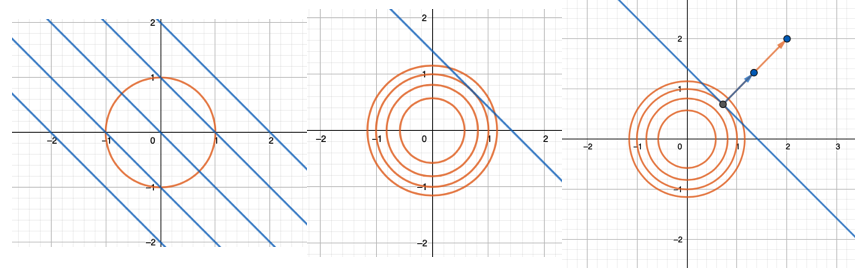
\includegraphics{images/level_set_0.png}
\caption{level\_set\_0.png}
\end{figure}

也就是上图最右,也就是:

\[
\nabla f = \lambda \nabla g
\]

而 拉格朗日乘数法 聪明的地方在于把 上述所有条件 pack在一个里面:

\[{\displaystyle {\begin{aligned}{\mathcal {L}}(x,y,\lambda )&=f(x,y) - \lambda \cdot g(x,y)\\[4pt]&=x+y - \lambda (x^{2}+y^{2}-1).\end{aligned}}}\]

求解:

\[
\frac{\partial \mathcal{L}}{\partial x} = 1 - 2 \lambda x = 0 \\
\frac{\partial \mathcal{L}}{\partial x} = 1 - 2 \lambda y = 0 \\
\frac{\partial \mathcal{L}}{\partial \lambda} = x^2 + y^2 - 1 = 0
\]

解出: \(\lambda = \pm\frac{1}{\sqrt{2}}\)

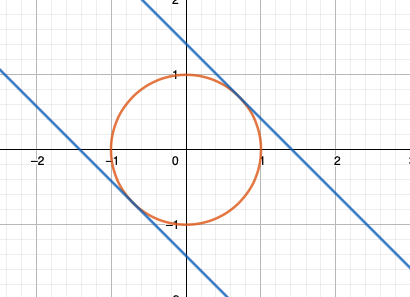
\includegraphics{images/min_max_point.png}

最值点:

\[
f(\frac{1}{\sqrt{2}}, \frac{1}{\sqrt{2}}) = \sqrt{2}\\
f(-\frac{1}{\sqrt{2}}, -\frac{1}{\sqrt{2}}) = -\sqrt{2}\\
\]

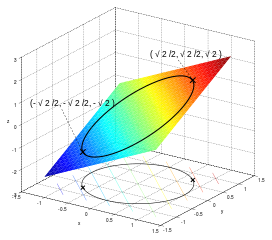
\includegraphics{images/272px-Lagrange_very_simple.png}

这个 \(\lambda\) 也是有物理意义的,比如 在 \(\lambda = \frac{1}{\sqrt{2}}\) 这里,它的物理意义是 假设 约束 有微小变化,此时 函数 f(x,y) 的变化.

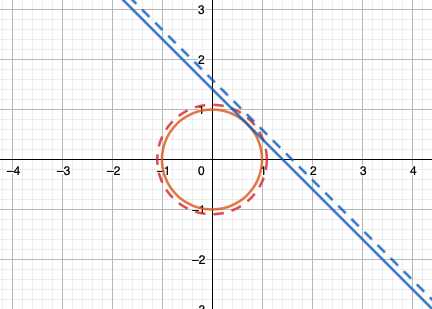
\includegraphics{images/lambda_meaning.png}

\begin{itemize}
\tightlist
\item
  例子二
\end{itemize}

\[
f(x,y) = x^2 y \\
\text{s.t. }  x^2 + y^2 = 3  \\
\]

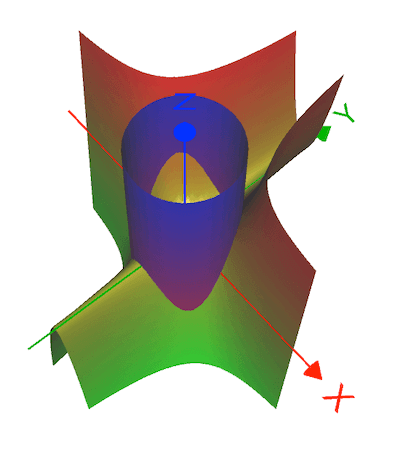
\includegraphics{images/lagrange_02.png}

\[{\displaystyle {\begin{aligned}{\mathcal {L}}(x,y,\lambda )&=f(x,y) - \lambda \cdot g(x,y)\\[4pt]&=x^2y - \lambda (x^{2}+y^{2}-3).\end{aligned}}}\]

求解:

\[
\frac{\partial \mathcal{L}}{\partial x} = 2xy - 2 \lambda x = 0 \\
\frac{\partial \mathcal{L}}{\partial x} = x^2 - 2 \lambda y = 0 \\
\frac{\partial \mathcal{L}}{\partial \lambda} = x^2 + y^2 - 3 = 0
\]

解出实际上有6个关键点,最终满足条件的最大最小值如下:

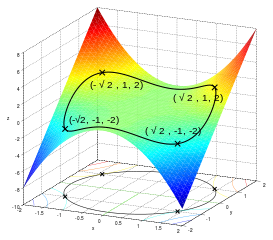
\includegraphics{images/273px-Lagrange_simple.png}

\begin{itemize}
\tightlist
\item
  例子三
\end{itemize}

假设我们有离散概率分布 \(\{p_{1},p_{2},\ldots ,p_{n}\}\), 想要具有最大的 信息熵:

\[
f(p_{1},p_{2},\ldots ,p_{n})=-\sum _{j=1}^{n}p_{j}\log _{2}p_{j} \\
\text{s.t. } g(p_{1},p_{2},\ldots ,p_{n})=\sum _{j=1}^{n}p_{j}=1
\]

同样构造

\[{\displaystyle {\begin{aligned}{\mathcal {L}}(x,y,\lambda )&=f(x,y) - \lambda \cdot g(x,y)\\[4pt]&= -\sum _{j=1}^{n}p_{j}\log _{2}p_{j} - \lambda (\sum _{j=1}^{n}p_{j} - 1)\end{aligned}}}\]

对每一个 \(p_k\) 求导:

\[
-\left({\frac {1}{\ln 2}}+\log _{2}p_{k}^{*}\right) - \lambda =0.
\]

最终可知:

\[
p_{k}^{*}={\frac {1}{n}}.
\]

均匀分布具有最大信息熵

\hypertarget{ux591aux4e2aux7ea6ux675f}{%
\section{多个约束}\label{ux591aux4e2aux7ea6ux675f}}

如果我们有多个约束,比如:

\[
f(x,y) \\
\text{s.t. } g_i(x) = 0, i = 1, \cdots , M
\]

那么我们的做法也是类似的,

\[
{\displaystyle {\mathcal {L}}\left(x_{1},\ldots ,x_{n},\lambda _{1},\ldots ,\lambda _{M}\right)=f\left(x_{1},\ldots ,x_{n}\right)-\sum \limits _{k=1}^{M}{\lambda _{k}g_{k}\left(x_{1},\ldots ,x_{n}\right)}} 
\]

\[
{\displaystyle \nabla _{x_{1},\ldots ,x_{n},\lambda _{1},\ldots ,\lambda _{M}}{\mathcal {L}}(x_{1},\ldots ,x_{n},\lambda _{1},\ldots ,\lambda _{M})=0\iff {\begin{cases}\nabla f(\mathbf {x} )-\sum _{k=1}^{M}{\lambda _{k}\,\nabla g_{k}(\mathbf {x} )}=0\\g_{1}(\mathbf {x} )=\cdots =g_{M}(\mathbf {x} )=0\end{cases}}}
\]

\hypertarget{ux4f8bux5b50-2}{%
\subsection{例子}\label{ux4f8bux5b50-2}}

给定约束: \(z^2 = x^2 + y^2 , x - 2z = 3\), 求满足约束的到原点的距离的极值, 约束条件如图:

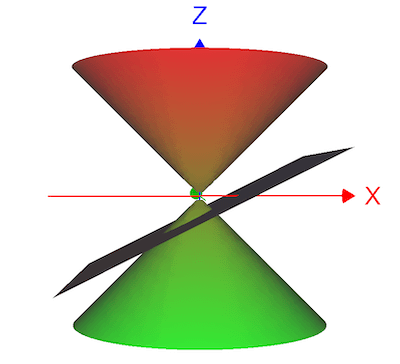
\includegraphics{images/Lagrange_03.png}

距离虽然是 \(d = \sqrt{x^2 + y^2 + z^2}\), 这里我们偷个懒,就用 \(f(x,y,z) = d^2\)

\[
f(x,y, z) = x^2 + y^2 + z^2 \\
x^2 + y^2 = z^2 \\
x - 2z = 3 \\
\]

计算:

\[{\displaystyle {\begin{aligned}{\mathcal {L}}(x,y,z,\lambda, \mu )&=f(x,y,z) - \lambda \cdot g(x,y,z) - \mu \cdot h(x,y,z) \\[4pt]&= x^2 + y^2 + z^2  - \lambda (x^2 + y^2 - z^2 ) - \mu(x - 2z -3) \end{aligned}}}\]

求解:

\[
\frac{\partial \mathcal{L}}{\partial x} = 2x -  2\lambda x - \mu = 0 \\
\frac{\partial \mathcal{L}}{\partial y} = 2y -  2\lambda y = 0 \\
\frac{\partial \mathcal{L}}{\partial y} = 2z +  2 \lambda z + 2\mu= 0 \\
\frac{\partial \mathcal{L}}{\partial \lambda} = x^2 + y^2 - z^2 = 0 \\
\frac{\partial \mathcal{L}}{\partial \mu} =  x - 2z -3  = 0
\]

最终按照以上条件可以解出:

\[
(-3, 0, 3) \to d_{max} = 3\sqrt{2} \\
(1, 0, -1) \to d_{min} = \sqrt{2}
\]

\hypertarget{kkt-ux6761ux4ef6}{%
\section{KKT 条件}\label{kkt-ux6761ux4ef6}}

\hypertarget{ux4ecbux7ecd-1}{%
\subsection{介绍}\label{ux4ecbux7ecd-1}}

KKT 条件(Karush--Kuhn--Tucker conditions) 则是更近一步,我们先考虑问题:

\[
f(x,y) \\
\text{s.t } g(\mathbf{x}) \le 0
\]

这个约束我们称之为 primal feasibility , 根据这个我们来定义 可行域 feasible region:

\[
K = \{ \mathbf{x} \in \mathbb{R}^n | g(\mathbf{x}) \le  0\}
\]

那么最优点 会有两种情况:

\begin{itemize}
\tightlist
\item
  \(g(\mathbf{x}) = 0\), 在边界,边界解(boundary solution),此时约束是有效的(active)
\item
  \(g(\mathbf{x}) < 0\), 在内部,内部解(interior solution),此时约束是无效的(inactive)
\end{itemize}

写出拉格朗日乘子:

\[\mathcal {L}(\mathbf{x},\lambda )=f(\mathbf{x}) + \lambda \cdot g(\mathbf{x})\\\]

然后分情况讨论:

\begin{itemize}
\tightlist
\item
  内部解,我们可以认为约束无效,所以可以认为条件是:
\end{itemize}

\[
\nabla f = \mathbf{0} \\
\lambda  = 0
\]

\begin{itemize}
\tightlist
\item
  边界解:
\end{itemize}

那就跟拉格朗日乘子法一样了,需要满足:

\[
g(\mathbf{x}) = 0 \\
\nabla f = -\lambda \nabla g
\]

这里的正负号是有意义的,我们希望最小化f, 而 \(\nabla f\) 指向的是 f 在 \(\mathbf{x}\) 的最陡上升方向,应该指向 可行域 的内部, 不过 \(\nabla g\) 指向 K 的外部,即 \(g(\mathbf{x}) > 0\) 的区域:

所以

\[
\lambda \ge 0 
\]

上面这个 \(\lambda \ge 0\) 条件称为 dual feasibility.

无论是边界解还是内部解,下面式子是一定满足的:

\[
\lambda g(\mathbf{x}) = 0
\]

这个条件 \(\lambda g(\mathbf{x}) = 0\) 称为 complementary slackness.

\hypertarget{kkt-ux6761ux4ef6-1}{%
\section{KKT 条件}\label{kkt-ux6761ux4ef6-1}}

我们可以总结上面的结论 再加上 等式约束:

Optimize

\[
f(\mathbf {x} )
\]

subject to

\[
{\displaystyle g_{i}(\mathbf {x} )\leq 0,}\\
{\displaystyle h_{i}(\mathbf {x} )=0.}
\]

\({\displaystyle g_{i}\ (i=1,\ldots ,m)}\) 为不等式约束, \({\displaystyle h_{i}\ (i=1,\ldots ,\ell )}\) 为等式约束。

\begin{itemize}
\tightlist
\item
  Stationarity
\end{itemize}

For maximizing \({\displaystyle \nabla f(x^{*})-\sum _{i=1}^{m}\mu _{i}\nabla g_{i}(x^{*})-\sum _{j=1}^{\ell }\lambda _{j}\nabla h_{j}(x^{*})=0,}\)

For minimizing : \({\displaystyle \nabla f(x^{*})+\sum _{i=1}^{m}\mu _{i}\nabla g_{i}(x^{*})+\sum _{j=1}^{\ell }\lambda _{j}\nabla h_{j}(x^{*})=0,}\)

\begin{itemize}
\tightlist
\item
  Primal feasibility
\end{itemize}

\[
{\displaystyle g_{i}(x^{*})\leq 0,{\text{ for }}i=1,\ldots ,m}\\
{\displaystyle h_{j}(x^{*})=0,{\text{ for }}j=1,\ldots ,\ell \,\!}
\]

\begin{itemize}
\tightlist
\item
  Dual feasibility
\end{itemize}

\({\displaystyle \mu _{i}\geq 0,{\text{ for }}i=1,\ldots ,m}\)

\begin{itemize}
\tightlist
\item
  Complementary slackness
\end{itemize}

\({\displaystyle \mu _{i}g_{i}(x^{*})=0,{\text{ for }}\;i=1,\ldots ,m.}\)

\hypertarget{ux4f8bux5b50-3}{%
\section{例子}\label{ux4f8bux5b50-3}}

\[
\text{minimize } x_1^2 + x_2^2 - 4x_1 - 4x_2 \\
\text{s.t } x_1^2 \le x_2 \\
x_1 + x_2 \le 2
\]

重写成:

\[
L(x_1, x_2, \mu_1, \mu_2) =  x_1^2 + x_2^2 - 4x_1 - 4x_2 + \mu_1(x_1^2 - x_2) + \mu_2( x_1 + x_2 - 2) \\
x_1^2 - x_ 2 \le 0 \\
x_1 + x_2 - 2 \le 0 \\
\mu_1 \ge 0 \\
\mu_2 \ge 0
\]

进一步:

\[
2x_1 + 2\mu_1x_1 + \mu_2 -4 = 0 \\
2x_2 - \mu_1 + \mu_2 - 4 = 0 \\
\mu_1(x_1^2 - x_2) = 0\\
\mu_2(x_1+x_2-2) = 0 \\
\mu_1, \mu_2 \ge 0
\]

尝试求解:

\begin{itemize}
\tightlist
\item
  \(\mu_1 = 0, x_1 + x_2 -2 = 0 \to x_2 = 1, x_1 = 1,\mu_2 = 2\)
\item
  \$\mu\_2 = 0, x\_1\^{}2 = x\_2 \to x\_1 = -2, x\_2 = 4, \mu\_1 = 4 \$
\item
  \(\mu_1 = \mu_2 = 0 \to x_1 = 2, x_2 = 2, x_2 = x_1^2\) 不可能\\
\item
  \(x_1^2 - x_2 = 0, x_1 + x_2 -2 = 0 \to x_1 = 1, x_1 = -2 \cdots\) 已经在以上情况中
\end{itemize}

最终最小值是在 f(1, 1) = -6

偏个题, 其实这里这个 \(f(x_1, x_2) = x_1^2 + x_2^2 - 4x_1 - 4x_2 = (x_1 -2)^ 2 + (x_2 - 2)^2 - 8\),如果把 \(x_1, x_2\) 用 x,y 来代替画图的话如下:

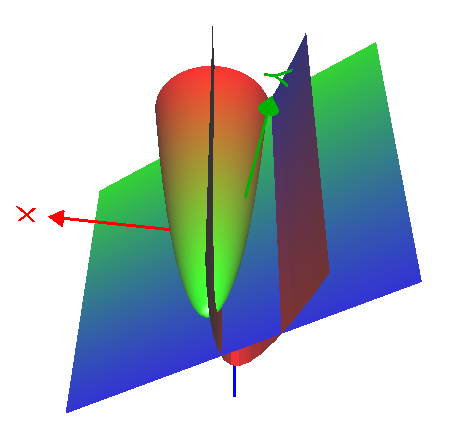
\includegraphics{images/kkt_ex01.png}

如果没有限制的话最小值是在 (2,2) 处取得,在有限制的情况下, (1, 1) 更靠近 (2,2), 所以也是合理的解。

\hypertarget{ux4eceux68afux5ea6ux4e0bux964dux5230ux5171ux8f6dux68afux5ea6-conjugate-gradient}{%
\chapter{从梯度下降到共轭梯度 \{Conjugate gradient\}}\label{ux4eceux68afux5ea6ux4e0bux964dux5230ux5171ux8f6dux68afux5ea6-conjugate-gradient}}

线性方程组 \(Ax =b\) 除了高斯消元法以外,还有一些很有趣的迭代解法, 比如雅可比法(Jacobi Method),高斯-赛德尔迭代(Gauss--Seidel method)。

这里只针对 A 满足 对称 (\(A^T = A\)), 正定(即 \({\displaystyle \forall {\vec {x}}\neq 0,{\vec {x}}^{T}A{\vec {x}}>0}\)),并且是实系数的,那么我们可以用 梯度下降 和共轭梯度来解线性方程组 :

\[Ax = b\]

\hypertarget{ux68afux5ea6ux4e0bux964d-gradient-descent}{%
\section{梯度下降 Gradient descent}\label{ux68afux5ea6ux4e0bux964d-gradient-descent}}

梯度下降(Gradient descent)完全配得上大名鼎鼎四个字,它这么大名鼎鼎是因为在 Machine Learning 中大放光彩。

\begin{quote}
梯度下降是用于找到可微函数的局部最小值的一阶迭代优化算法。 为了使用梯度下降找到函数的局部最小值,我们采取与该函数在当前点的梯度(或近似梯度)的负值成比例的步骤。 但是,如果我们改为采取与梯度的正比成比例的步骤,则会逼近该函数的局部最大值。 该过程称为梯度上升。
\end{quote}

梯度下降本身的数学原理还是比较简单,还有这里虽然叫 `梯度下降' 来找局部最小值,其实我们走的是 梯度 的负方向,因为 梯度 本身指向的方向是函数 \(f: \mathbb{R}^n \to \mathbb{R}\) 增加的最快的方向。

\begin{quote}
就像一元函数的导数表示这个函数图形的切线的斜率,如果多元函数在点 P 上的梯度不是零向量,它的方向是这个函数在 P 上最大增长的方向,而它的量是在这个方向上的增长率。
\end{quote}

考虑函数:

\[
f(\vec{x}) = \frac{1}{2} \vec{x}^TA\vec{x} - \vec{b}^T \vec{x} + c
\]

如果我们要求 \(f(\vec{x})\) 的最小值,那么:

\[
 \nabla f(\vec{x}) = A\vec{x} - \vec{b}
\]

梯度下降法要做的是:

\begin{itemize}
\tightlist
\item
  \(\vec{d}_k = -\nabla f(\vec{x}_{k-1}) = \vec{b} - A \vec{x}_{k-1}\)
\item
  \(\vec{x}_k = \vec{x}_{k-1} + \alpha_k \vec{d}_k\), 选择最合适的 \(\alpha_k\) 使得 \(f(\vec{x}_k) < f(\vec{x}_{k-1})\)
\end{itemize}

对于 \(\alpha_k\):

\[
\begin{aligned}
g(\alpha) &= f(\vec{x} + \alpha \vec{d})  \\
&= \frac{1}{2} (\vec{x} + \alpha \vec{d})^T A (\vec{x} + \alpha \vec{d}) - \vec{b}^T (\vec{x} + \alpha \vec{d}) + c \\
&= \frac{1}{2} (\vec{x}^T A \vec{x} + 2 \alpha \vec{x}^T A \vec{d} + \alpha^2 \vec{d}^T A \vec{d}) - \vec{b}^T \vec{x} - \alpha \vec{b}^T \vec{d} + c \\
&= \frac{1}{2} \alpha^2 \vec{d}^T A \vec{d} + \alpha (\vec{x}^TA\vec{d} - \vec{b}^T\vec{d}) + const
\end{aligned}
\]

对 \(\alpha\) 求导:

\[
\begin{aligned}
\frac{d g(\alpha)}{d \alpha} &= \alpha \vec{d}^T A \vec{d} + (\vec{x}^TA\vec{d} - \vec{b}^T\vec{d}) \\
&= \alpha \vec{d}^T A \vec{d} + \vec{d}^T A\vec{x} - \vec{d}^T \vec{b} \\
&= \alpha \vec{d}^T A \vec{d} + \vec{d}^T (A\vec{x} - \vec{b})
\end{aligned}
\]

令上面的式子为0:

\[
\alpha =  \frac{\vec{d}^T (\vec{b} - A\vec{x} ) } {\vec{d}^TA\vec{d}}
\]

有 \(\vec{d}_k = \vec{b} - A \vec{x}_{k-1}\), 所以:

\[
\alpha_k =  \frac{\vec{d}_k^T \vec{d}_k } {\vec{d}^T_kA\vec{d}_k}
\]

总结算法:

\[
\vec{d}_k = \vec{b} - A \vec{x}_{k-1} \\
\alpha_k =  \frac{\vec{d}_k^T \vec{d}_k } {\vec{d}^T_kA\vec{d}_k} \\
\vec{x}_k = \vec{x}_{k-1} + \alpha_k \vec{d}_k
\]

这个算法本身不是特别常用,它的收敛速度取决于 \(AA^T\) 的最大与最小特征值之比。

\hypertarget{ux5171ux8f6dux68afux5ea6-conjugate-gradient}{%
\section{共轭梯度 Conjugate gradient}\label{ux5171ux8f6dux68afux5ea6-conjugate-gradient}}

为什么梯度下降没有那么常用呢? 因为我们有共轭梯度。

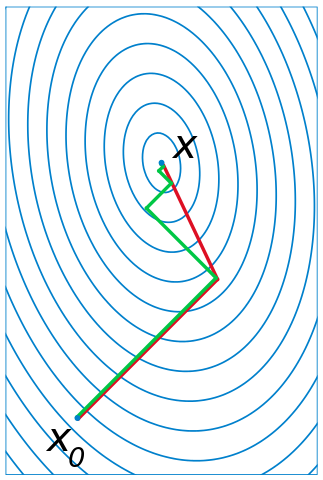
\includegraphics{images/323px-Conjugate_gradient_illustration.png}

绿色是梯度下降的路线,红色是共轭梯度的路线,明显共轭梯度走的次数少一些/更快收敛。

梯度下降在下降的过程中会走 z 字,感性的想一想这是合理的,比如我在这个方向走到最多的下降的,再朝这个方向走我们就不是下降了,所以当然我们接下来就会走朝它垂直的方向。

而共轭梯度,它好像更聪明一点,在这张图中,n = 2, 走完第一步,下一步它就直接走到了最小值。

作为更像call 共轭梯度 API 的人,暂时我也没有完全数学的理解它,下面这个链接有具体的背景和数学推导:

\href{https://flat2010.github.io/2018/10/26/共轭梯度法通俗讲义/}{共轭梯度法通俗讲义}

感性的理解一下,就是共轭梯度这里的关键是需要理解`共轭(conjugate)',向量 \(\vec{u}\) 和 \(\vec{v}\) 是共轭的 (相对于A )如果满足:

\[
\vec{u} ^{\mathsf {T}}\mathbf {A} \vec {v} =0.
\]

下面这张图,里面的两两向量都是针对所在梯度处的矩阵`共轭'的:

\begin{figure}
\centering
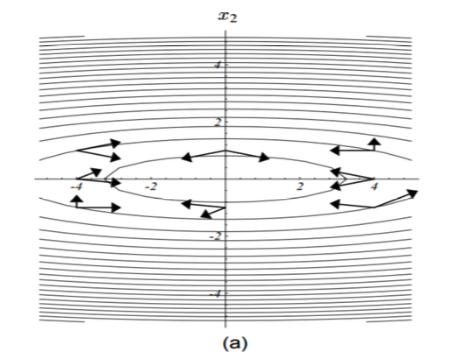
\includegraphics{images/conjugate_02.png}
\caption{conjugate\_02.png}
\end{figure}

当我们把梯度变换一下,就更明显的看出`共轭'其实也就是某种正交:

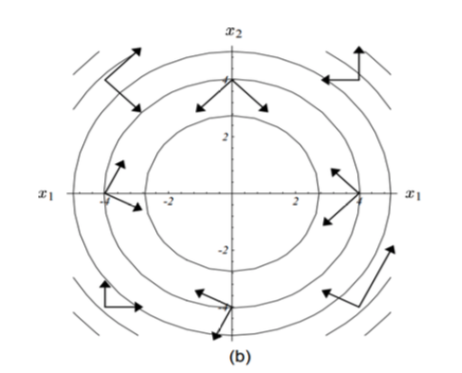
\includegraphics{images/conjugate_01.png}

这种正交带给我们的好处是更甚于上面的梯度下降的,我们可以一次在某个共轭的方向走到头,然后下一次就无需再走走过的共轭方向。

算法-from wikipedia:

\[
\begin{aligned}
& \mathbf{r}_0 := \mathbf{b} - \mathbf{A x}_0 \\
& \hbox{if } \mathbf{r}_{0} \text{ is sufficiently small, then return } \mathbf{x}_{0} \text{ as the result}\\
& \mathbf{p}_0 := \mathbf{r}_0 \\
& k := 0 \\
& \text{repeat} \\
& \qquad \alpha_k := \frac{\mathbf{r}_k^\mathsf{T} \mathbf{r}_k}{\mathbf{p}_k^\mathsf{T} \mathbf{A p}_k}  \\
& \qquad \mathbf{x}_{k+1} := \mathbf{x}_k + \alpha_k \mathbf{p}_k \\
& \qquad \mathbf{r}_{k+1} := \mathbf{r}_k - \alpha_k \mathbf{A p}_k \\
& \qquad \hbox{if } \mathbf{r}_{k+1} \text{ is sufficiently small, then exit loop} \\
& \qquad \beta_k := \frac{\mathbf{r}_{k+1}^\mathsf{T} \mathbf{r}_{k+1}}{\mathbf{r}_k^\mathsf{T} \mathbf{r}_k} \\
& \qquad \mathbf{p}_{k+1} := \mathbf{r}_{k+1} + \beta_k \mathbf{p}_k \\
& \qquad k := k + 1 \\
& \text{end repeat} \\
& \text{return } \mathbf{x}_{k+1} \text{ as the result}
\end{aligned}
\]

wikipedia 上也能找到 共轭梯度法 的 MATLAB 代码。

这个知乎回答也很好:

\url{https://www.zhihu.com/question/27157047/answer/121950241}

\hypertarget{ux603bux7ed3}{%
\section{总结}\label{ux603bux7ed3}}

针对

\[
Ax = b
\]

因为 A 的不同性质,我们可以有不同的选择:

\begin{itemize}
\tightlist
\item
  矩阵稠密,或者数量级较小(dense and/or small): 高斯消元法
\item
  矩阵稀疏,数量级很大(large and sparse, or not available ex- plicitly):如果矩阵没有一些特殊的性质(实对称正定),那一般来说是没什么好的办法,考虑使用迭代法
\item
  带状矩阵(narrow-banded):要看是那种带状,如果是比如这样,只有对角线和对角线上方和下面的一条或者两条,那么高斯消元法应该还行:
\end{itemize}

Tridiagonal matrix:

\[
\begin{pmatrix}
a_1 & b_1 \\
c_1 & a_2 & b_2 \\
& c_2 & \ddots & \ddots \\
& & \ddots & \ddots & b_{n-1} \\
& & & c_{n-1} & a_n
\end{pmatrix}
\]

Pentadiagonal matrix:

\[
{\displaystyle {\begin{pmatrix}c_{1}&d_{1}&e_{1}&0&\cdots &\cdots &0\\b_{1}&c_{2}&d_{2}&e_{2}&\ddots &&\vdots \\a_{1}&b_{2}&\ddots &\ddots &\ddots &\ddots &\vdots \\0&a_{2}&\ddots &\ddots &\ddots &e_{n-3}&0\\\vdots &\ddots &\ddots &\ddots &\ddots &d_{n-2}&e_{n-2}\\\vdots &&\ddots &a_{n-3}&b_{n-2}&c_{n-1}&d_{n-1}\\0&\cdots &\cdots &0&a_{n-2}&b_{n-1}&c_{n}\end{pmatrix}}\,.}
\]

但是如果是类似带状,但是还有一些其它的非0项在矩阵中的话,那么我们就需要考虑矩阵的性质了。

\begin{itemize}
\tightlist
\item
  实对称正定,稠密,数量级小(symmetric positive definite,dense and/or small): Cholesky 分解
\item
  实对称正定,稀疏,数量级大(symmetric positive definite,large and sparse): 毫无疑问,共轭梯度!
\item
  对称不定,稠密,数量级小(symmetric indefinite, dense and/or small):Bunch--Kaufman
\item
  对称不定,稀疏,数量级大(symmetric indefinite, large and sparse): MINRES
\item
  不对称,稀疏,数量级大(nonsymmetric, large and sparse): GMRES,BiCGSTAB or IDR
\end{itemize}

参考:

\begin{itemize}
\tightlist
\item
  \url{https://en.wikipedia.org/wiki/Gradient_descent}
\item
  \url{https://en.wikipedia.org/wiki/Conjugate_gradient_method}
\item
  Solution of Linear Systems via Chen Greif
\end{itemize}

\hypertarget{ux63d2ux503c-interpolate}{%
\chapter{插值 \{Interpolate\}}\label{ux63d2ux503c-interpolate}}

其实之前写B样条就多处涉及到插值。但是这里还是简单总结一下有关插值,首先插值是给我们一些点,想让我们重建整个函数,这样给我们新的点,我们可能也可以做预测之类的,可以让我们从有限维到无限维。

插值最简单/方便的理解方式就是有一组基 \(\phi_1, \phi_2, \cdots\):

\[
f(x) = \sum_i a_i \phi_i(x)
\]

其中 a 是我们要求的。

以下讨论针对 k 个点 \((x_1, y_1), \cdots, (x_k, y_k)\) 满足 \(x_1 < x_2 < \cdots < x_k\)

\hypertarget{ux591aux9879ux5f0fux63d2ux503c}{%
\section{多项式插值}\label{ux591aux9879ux5f0fux63d2ux503c}}

最简单的就是多项式插值:

\[
f(x) = a_0 + a_1x + a_2 x^2 + \cdots + a_{k-1} x^{k-1}
\]

我们可以写出方程:

\[
\begin{bmatrix}
1 & x_1  & \ldots & x_1^{k-1} \\
1 & x_2  & \ldots & x_2^{k-1} \\
\vdots & \vdots    & \vdots    &  \vdots   \\
1 & x_{k-1}  & \ldots & x_k^{k-1} \\
\end{bmatrix}
\begin{bmatrix} a_0 \\ a_1  \\ \vdots \\ a_{k-1} \end{bmatrix}  =
\begin{bmatrix} y_1 \\ y_2  \\ \vdots \\ y_k \end{bmatrix}
\]

这里的已知是 x,y 要求的是 a, 求解线性方程组,既可得到答案。

多项式插值的问题肉眼可见,那就是基

\[
\{1, x, x^2, \cdots, x^{k-1}\}
\]

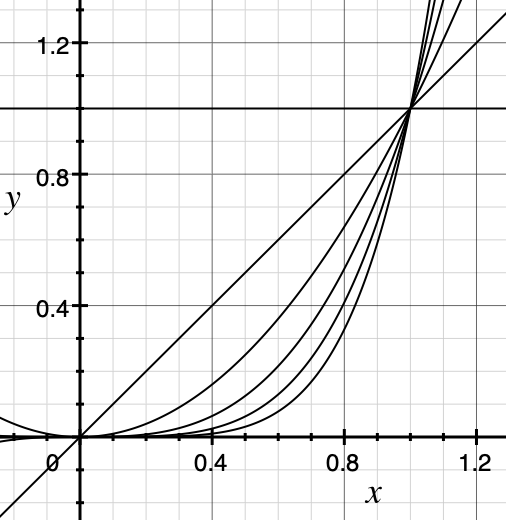
\includegraphics{images/poly_basis.png}

明显不是一组很好的基。而且正如 B样条 中写过,多项式次数高,会波动很大。

\hypertarget{ux62c9ux683cux6717ux65e5ux63d2ux503cux6cd5}{%
\section{拉格朗日插值法}\label{ux62c9ux683cux6717ux65e5ux63d2ux503cux6cd5}}

另一种多项式插值方法是把基选择为:

\[
\phi_i(x) = \frac{\prod_{j \ne i} (x - x_j)}{\prod_{j \ne i} (x_i - x_j)}
\]

基满足:

\[
\phi_i(x_l) = \begin{cases}
      1, l = i\\
      0, otherwise
\end{cases}
\]

针对 拉格朗日 插值法一种简单的理解就是 多项式 * 多项式 依旧是多项式,而它的基也就是这样定的。用一个具体的例子,比如三个点会更加容易理解拉格朗日插值法。

这种多项式插值的问题在于:计算大,同时如果有两个点很靠近的话 \(x_i \approx x_j\), 计算就会有较大的问题。当然上面提到的多项式插值的问题它也依旧存在。

多项式插值还有的问题包括:比如我们增加一个点,或者改变一个点,会对所有的系数a都产生影响,所以有了牛顿插值法。

\hypertarget{ux725bux987fux63d2ux503cux6cd5}{%
\section{牛顿插值法}\label{ux725bux987fux63d2ux503cux6cd5}}

牛顿插值法的基我们写成:

\[
\phi_i(x) = \prod_{j = 1}^{i - 1} (x - x_j)
\]

其中

\[
\phi_1(x) = 1
\]

容易看出:

\[
\phi_i(x_l) = 0, l < i
\]

牛顿插值法的关键之处就是 我们只考虑跟它前面有关的点, 我们展开 \(f(x) = \sum_i a_i \phi_i(x)\) 可得线性方程组:

\[
\begin{bmatrix}
\phi_1(x_1) & 0  & \ldots & 0 \\
\phi_1(x_1) & \phi_2(x_2)  & \ldots & 0 \\
\vdots & \vdots    & \vdots    &  \vdots   \\
\phi_1(x_1) & \phi_2(x_2)  & \ldots & \phi_k(x_k) \\
\end{bmatrix}
\begin{bmatrix} a_1 \\ a_2  \\ \vdots \\ a_k \end{bmatrix}  =
\begin{bmatrix} y_1 \\ y_2  \\ \vdots \\ y_k \end{bmatrix}
\]

除了上面这些常见的插值基以外,我们还可以有,比如:

\[
f(x) = \frac{p_0 + p_1x + p_2 x^2 + \cdots + p_m x^m}{q_0 + q_1x + q_2 x^2 + \cdots + q_n x^n}
\]

\hypertarget{ux5206ux6bb5ux63d2ux503c}{%
\section{分段插值}\label{ux5206ux6bb5ux63d2ux503c}}

分段插值可以说是 spline 的灵魂所在,感觉分段插值的好处是 local 性比较好,添加/减少/改变一个点 不会对全局影响那么高,个人感觉有限元的基础也是线性分段插值。

插值之所以重要是前面提到了,它可以某种程度让我们有限到无限,给一些点,我们可以插值(interpolate ),可以外推(extrapolate),而计算机图形学中插值又无处不在,可以涉及到 linear, bilinear, trilinear, bicubic, 也就是一个插值,让我们能从三角形 mesh 能渲染出好看的场景,玩出无数的花样。

\hypertarget{ux6570ux503cux79efux5206ux548cux5faeux5206numerial-intergration}{%
\chapter{数值积分和微分\{Numerial Intergration\}}\label{ux6570ux503cux79efux5206ux548cux5faeux5206numerial-intergration}}

\hypertarget{ux79efux5206}{%
\section{积分}\label{ux79efux5206}}

针对 \(f: \mathbb{R} \to \mathbb{R}\)

\hypertarget{ux9eceux66fcux548c}{%
\subsection{黎曼和}\label{ux9eceux66fcux548c}}

记得我第一次看 黎曼和/黎曼积分 的时候觉得真是有意思,觉得这个东西很不言自明,我们推推导积分的时候从有限小到无限小,而当我们为了计算机计算,又从无穷小到可衡量的有限小。有意思。

积分也就是求和。而且觉得这一切都和 中值定理 有着千丝万缕的联系,o(╯□╰)o :

\begin{quote}
对一个在闭区间 {[}a,b{]}有定义的实值函数f, f关于取样分割\$ x\_\{0\},\ldots ,x\_\{n\}、t\_\{0\},\ldots ,t\_\{n-1\}\$ 的黎曼和(积分和)定义为以下和
\end{quote}

\begin{quote}
\[
\sum _{i=0}^{n-1}f(t_{i})(x_{i+1}-x_{i})
\]
\end{quote}

\begin{quote}
和式中的每一项是子区间长度 \$ x\_\{i+1\}-x\_\{i\}\$ 与在 \(t_{i}\) 处的函数值 \(f(t_{i})\) 的乘积。直观地说,就是以标记点 \(t_{i}\) 到 X轴 的距离为高,以分割的子区间为长的矩形的面积。
\end{quote}

\begin{figure}
\centering
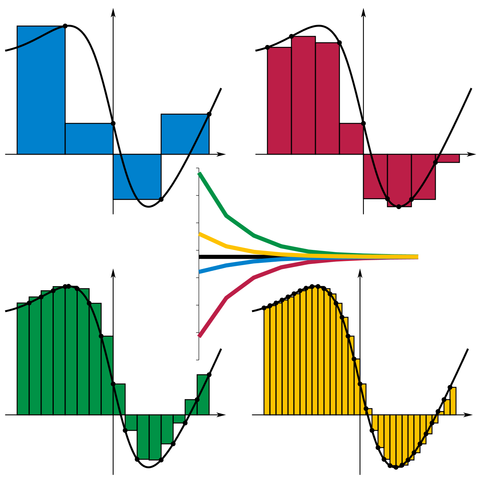
\includegraphics{images/480px-Riemann_sum_convergence.png}
\caption{图片来自wikipedia}
\end{figure}

在上图中, \(f(t_i)\) 选择分别为 左端、右端、极小值、极大值。

\hypertarget{ux68afux5f62ux6cd5ux5219}{%
\subsection{梯形法则}\label{ux68afux5f62ux6cd5ux5219}}

在一个`小区间'我们就能玩出很多花样:

\includegraphics{images/365px-Trapezoidal_rule_illustration.png}

比如我们如果取两端来估算 面积 的话:

\[{\displaystyle \int \limits _{a}^{b}f(x)dx\approx {\frac {b-a}{2}}[f(a)+f(b)]}\]

我们也可以取区间中点的高度来估计 面积:

\[{\displaystyle \int \limits _{a}^{b}f(x)dx\approx (b-a)f({\frac {a+b}{2}})}\]

以上都被称为 梯形法则(Trapezoidal rule),这里可以是整个函数,也可以只是一个小区间,我们可以用黎曼和来对待小区间:

\begin{enumerate}
\def\labelenumi{\arabic{enumi}.}
\tightlist
\item
  分割许多小区间
\item
  把小区间加起来
\end{enumerate}

\includegraphics{images/320px-Trapezoidal_rule_illustration_small.png}

\hypertarget{ux8f9bux666eux68eeux6cd5ux5219}{%
\subsection{辛普森法则}\label{ux8f9bux666eux68eeux6cd5ux5219}}

\begin{quote}
辛普森法则(Simpson's rule)是一种数值积分方法,是牛顿-寇次公式的特殊形式,以二次曲线逼近的方式取代矩形或梯形积分公式,以求得定积分的数值近似解。其近似值如下:
\end{quote}

\[\int_{a}^{b} f(x) \, dx \approx \frac{b-a}{6}\left[f(a) + 4f\left(\frac{a+b}{2}\right)+f(b)\right]\]

\includegraphics{images/Simpsons_method_illustration.png}

辛普森法则可以令 \(f(x) = A x^2 + Bx + C\) 然后推导出来。

同样也可以分割小区间然后求和。

实际上上面两种无非是采取了不不同的近似,梯形法则 使用直线来近似原函数, 辛普森法则 使用二次曲线来 近似原函数。它们都是 牛顿-柯特斯公式(Newton-Cotes rule / Newton-Cotes formula) 的特殊形式。

\hypertarget{ux725bux987f-ux67efux7279ux65afux516cux5f0f}{%
\subsection{牛顿-柯特斯公式}\label{ux725bux987f-ux67efux7279ux65afux516cux5f0f}}

还有一些有趣的看法,比如我们始终是利用 n 个离散的点的值来得到积分结果 - 一个数字,那么积分总可以写成这样:

\[\int _{a}^{b}f(x)\,dx\approx \sum _{{i=0}}^{n}w_{i}\,f(x_{i})\]

这种看法的原理是:

\begin{itemize}
\tightlist
\item
  假设已知 \(f(x_{0}),f(x_{1}),\dots ,f(x_{n})\) 的值。
\item
  以n+1点进行插值,求得对应 f(x)的拉格朗日多项式。
\item
  对该n次的多项式求积。
\end{itemize}

该积分便可以作为 \(\int _{a}^{b}f(x)\,dx\) 的近似,而由于该拉格朗日多项式的系数都是常数(由n决定其值),所以积函数的系数(即 \(w_{i}\))都是常数。

或者就这样写:

\[
\begin{aligned}
\int_a^b f(x)dx &= \int_a^b \bigg[ \sum_i a_i \phi_i(x)\bigg] dx  \\
&=\sum_i a_i \bigg[ \int_a^b  \phi_i(x)\bigg] dx\\
&= \sum_i c_i a_i, \text{ for } c_i \equiv \int_a^b \phi_i(x) dx
\end{aligned}
\]

然后我们就可以写出方程组:

\[
w_1 \cdot 1 + w_2 \cdot 2 + \cdots + w_n \cdot 1 = \int_a^b 1dx = b - a \\
w_1 \cdot x_1 + w_2 \cdot x_2 + \cdots + w_n \cdot x_n = \int_a^b xdx = (b^2 - a^2)/2 \\
\vdots \\
w_1 \cdot x_1^{n-1} + w_2 \cdot x_2^{n-1} + \cdots + w_n \cdot x_n^{n-1} = \int_a^b x^{n-1}dx = (b^n - a^n)/n \\
\]

然后也就是一个解线性方程组的问题。

这个方法明显会有 高阶多项式震荡的厉害的 龙格现象, 我还是更喜欢拆小区间,然后再组合小区间的做法。

\hypertarget{ux7cbeux786eux5ea6}{%
\subsection{精确度}\label{ux7cbeux786eux5ea6}}

用 拆小区间再复合 梯形法则的精确度是 \(O(\Delta x^3)\), 辛普森 的精确度是 \(O(\Delta x^4)\)

针对 \(f: \mathbb{R}^k \to \mathbb{R}\), 好像针对多元函数,蒙特卡洛积分比较常见/用一点。

\hypertarget{ux5faeux5206}{%
\section{微分}\label{ux5faeux5206}}

关于微分,我们首先也可以用插值类似的思想来看

\[
f'(x) = \sum_i a_i \phi_i'(x)
\]

这是有限元的思想。

当然更简单的就是我们直接从定义入手:

\[
f'(x) = \lim_{h \to 0} \frac{f(x+h) - f(x)}{h}
\]

选择比较小的h, 得到 前向差分公式:

\[
f'(x) \approx  \frac{f(x+h) - f(x)}{h}
\]

也可以从 x 向后 得到 后向差分公式:

\[
f'(x) \approx \frac{f(x) - f(x-h)}{h}
\]

以上两个式子本质都是用的泰勒展开:

\[
f(x+h) = f(x) + f'(x) h + \frac{1}{2} f''(x) h^2 + \cdots
\]

精度为 O(h):

\[
f'(x) = \frac{f(x+h) - f(x)}{h} + O(h)
\]

或者我们可以用下面的办法展开:

\[
f(x+h) = f(x) + f'(x) h + \frac{1}{2} f''(x) h^2 + \frac{1}{6}f'''(x)h^3 + \cdots  \tag{1}\\
\]

\[
f(x-h) = f(x) - f'(x) h + \frac{1}{2} f''(x) h^2 - \frac{1}{6}f'''(x)h^3 + \cdots  \tag{2}
\]
上下两式相减:

\[
f(x+h) - f(x -h) = 2f'(x) + \frac{1}{3}f'''(x)h^3 + \cdots 
\]

这叫做 中点差分公式, 精度是 \(O(h^2)\)

\[
f'(x)  \approx \frac{f(x+h) - f(x-h)}{2h}
\]

我们也可以用(1),(2)式得到二阶导数的 O(h) 中点差分公式:

\[
f''(x) \approx \frac{f(x+h) - 2f(x) +  f(x-h)}{h^2}
\]

我们可以利用 理查德森外推法 来提高 二阶导的精度:

\[
D(h) = \frac{f(x+h) - f(x)}{h} = f'(x) + \frac{1}{2} f''(x) h + O(h^2)
\]

对于任意 \(\alpha\) ,我们可以有 \(D(h), D(\alpha h)\):

\[
D(h) = f'(x) + \frac{1}{2} f''(x) h + O(h^2) \\
D(\alpha h) = f'(x) + \frac{1}{2} f''(x) \alpha h + O(h^2) \\
\]

写成矩阵形式:

\[
 \begin{pmatrix} D(h) \\ D(\alpha h) \end{pmatrix}   = \begin{pmatrix} 1 & \frac{1}{2}h  \\ 1 & \frac{1}{2}\alpha h  \end{pmatrix}\begin{pmatrix} f'(x) \\ f''(x) \end{pmatrix}   + O(h^2)
\]

\[
\begin{pmatrix} f'(x) \\ f''(x) \end{pmatrix} = \begin{pmatrix} 1 & \frac{1}{2}h  \\ 1 & \frac{1}{2}\alpha h   \end{pmatrix}^{-1}  \begin{pmatrix} D(h) \\ D(\alpha h) \end{pmatrix}  + O(h^2)
\]

这样可以以解出精度为 \(O(h^2)\) 的 f'(x):

\[
f'(x) = \frac{1}{1- \alpha}(-\alpha D(h) + D(\alpha h)) + O(h^2)
\]

参考:

\begin{itemize}
\tightlist
\item
  \href{https://zh.wikipedia.org/wiki/差分\#單位步長情況}{差分}
\item
  \href{https://zh.wikipedia.org/wiki/理查德森外推法}{理查德森外推法}
\item
  \href{https://zh.wikipedia.org/wiki/牛頓-寇次公式}{牛顿-柯特斯公式}
\item
  \href{https://en.wikipedia.org/wiki/Taylor_series}{Taylor series}
\item
  \href{https://en.wikipedia.org/wiki/Riemann_sum}{Riemann\_sum}
\item
  \href{https://en.wikipedia.org/wiki/Trapezoidal_rule}{Trapezoidal rule}
\item
  \href{https://en.wikipedia.org/wiki/Simpson\%27s_rule}{Simpson's rule}
\end{itemize}

数值积分和微分当然非常有用,中文翻译的 差分 也很合适,其实数值积分和微分就是 求和 和 差分。这当然很重要,有了 积分和微分(求和和差分)才能帮我们把一些数学方程/模型方便的用到计算机上。

比如 渲染领域 的蒙特卡洛积分。

然后发现 Scipy 也提供 integrate, 可以查看: \href{http://liao.cpython.org/scipy18/}{SciPy求函数的积分}

\hypertarget{ux5e38ux5faeux5206ux65b9ux7a0b-ode}{%
\chapter{常微分方程 \{ODE\}}\label{ux5e38ux5faeux5206ux65b9ux7a0b-ode}}

微分方程- 即使只是常微分方程( ordinary differential equation, ODE) 也是非常有趣的。

比如牛顿第二定律:

\[
m\frac{d^2 x}{d t^2} = F(x)
\]

比如大名鼎鼎的 logistic function:

\[\frac{dP}{dt} = P\]

\hypertarget{ux57faux672cux5f62ux5f0f}{%
\section{基本形式}\label{ux57faux672cux5f62ux5f0f}}

\[
F(t): \mathbb{R} \to \mathbb{R}^n \\
\text{satifying }: F[t, f(t), f'(t), f''(t), \cdots, f^{(k)}(t)] = 0 \\
\text{Given } f(0), f'(0), f''(0), \cdots, f^{(k-1)}(0)
\]

给我们上面的式子,希望我们能推导出 \(f(t), f'(t), \cdots, f^{(k)}(t)\) 随着时间 t 的变化。

\begin{itemize}
\tightlist
\item
  显式 vs 隐式
\end{itemize}

上面这个事实叫做 n 阶隐式(implicit)常微分方程,有的时候我们可以把它化为显式 (explicit)的:

\[
f^{(k)}(t) = F[t, f(t), f'(t), f''(t), \cdots, f^{(k-1)}(t)] 
\]

比如上面的两个例子都是显式的。

\begin{itemize}
\tightlist
\item
  自治 vs 非自治
\end{itemize}

自治(autonomous) 系统形式如下,一般来说,也就是 f 与时间无关:

\[
\frac{d}{dt}x(t)=f(x(t))
\]

比如上面我们的牛顿第二定律, 非自治形式如下:

\[
{\displaystyle {\frac {d}{dt}}x(t)=g(x(t),t)}
\]

物理上来说,这表示空间中一点的性质不仅取决于它的位置,还取决于时间:在不同的时间,经过此一点的质点或粒子会受到不同的影响。

\begin{itemize}
\tightlist
\item
  其它
\end{itemize}

当然常微分方程还有许多其它的分类,比如线性、齐次等.

\hypertarget{ux663eux5f0f-ode}{%
\section{显式 ODE}\label{ux663eux5f0f-ode}}

假设我们有 ODE 如下:

\[
y''' = 3y'' - 2y' + y
\]

因为有:

\[
\frac{d^2 y}{d t^2} = \frac{d}{dt} \bigg( {\frac{dy}{dt}} \bigg)\\
\]

我们令:

\[
z = \frac{dy}{dt}\\
w = \frac{d^2 y}{d t^2}
\]

我们可以把上面的式子写成:

\[
\frac{d}{d t}\begin{pmatrix} y \\ z \\ w \end{pmatrix} =  \begin{pmatrix} 0 & 1 & 0 \\ 0 & 0 & 1 \\ 1 & -2 & 3 \end{pmatrix}\begin{pmatrix} y \\ z \\ w \end{pmatrix} 
\]

我们可以把显式的 ODE 转化成一阶ODE。更一般的,对于显式 ODE:

\[f^{(k)}(t) = F[t, f(t), f'(t), f''(t), \cdots, f^{(k-1)}(t)] 
\]

我们都可以把之转化成一阶 ODE:

\[
\frac{d}{d t}\begin{pmatrix} g_1(t) \\ g_2(t) \\ \vdots \\ g_{k-1}(t) \\ g_k(t) \end{pmatrix} = \begin{pmatrix} g_2(t) \\ g_3(t)\\  \vdots \\ g_k(t) \\ F[t, g_1(t), g_2(t),  \cdots, g_{(k-1)}(t)]  \end{pmatrix} 
\]

上面这个式子中: \(g_2(t) = g_1'(t), g_3(t) = g_2'(t) = g_1''(t)\).

更好的是,我们可以把显式的微分方程转化为自治的,如果有: \(f'(t) = F[t, f(t)]\), 我们令 \(g(t) = t\), 则 \(f'(t)\) 可以写成:

\[
\frac{d}{d t}\begin{pmatrix} g(t) \\ f(t) \end{pmatrix} = \begin{pmatrix} 1 \\ F[g(t), f(t)] \end{pmatrix} 
\]

所以我们只需要考虑一阶自治ODE,即:

\[
f'(t) = F[f(t)]
\]

\hypertarget{ux53efux89c6ux5316}{%
\section{可视化}\label{ux53efux89c6ux5316}}

如果我们想可视化ODE,一般会使用两种方法。

\begin{itemize}
\tightlist
\item
  斜率场 slope field
\end{itemize}

\begin{quote}
A slope field is a collection of short line segments, whose slopes match that of a solution of a first-order differential equation passing through the segment's midpoint. The pattern produced by the slope field aids in visualizing the shape of the curve of the solution. This is especially useful when the solution to a differential equation is difficult to obtain analytically.
\end{quote}

\begin{figure}
\centering
\includegraphics{images/Slope_Field.png}
\caption{Slope\_Field.png}
\end{figure}

上图画的是斜率场为:

\[
\frac{dy}{dx} = x^2 - x - 2
\]

其中 蓝、红、青 的线条分别是:

\[
x^3/3 - x^2/2 -2x+4 \\
x^3/3 - x^2/2 -2x \\
x^3/3 - x^2/2 -2x-4
\]

肉眼可以某种程度的看出它们满足这个斜率场。

当然这是极好的状况,有时候即使算不出来解析解,我们画出这个斜率场也能某种程度的了解我们的ODE变化情况。

\begin{itemize}
\tightlist
\item
  相图 phase diagram
\end{itemize}

\includegraphics{images/phase_diagram_2.png}

比如看上面这个 \(dx/dt = f(x)\):

\[
\frac{dx}{dt} = x(1-x)
\]

因为它是自治的, 所以斜斜率场的斜率不会随着时间变化, 在 x = 0 与 x = 1 处 有 \(dx/dt = 0\), 然后自然而然的就是画出右边的 phase line,可以容易看出它的平衡点与平衡状态。

\hypertarget{ux89e3ux7684ux72b6ux51b5}{%
\section{解的状况}\label{ux89e3ux7684ux72b6ux51b5}}

对于 \(y' = 2y/t\):

\[
\frac{dy}{dt} = \frac{2y}{t}
\]

通过分离变量法可以解的:

\[
ln |y| = 2 ln t + c
\]

或者写成: \(y = Ct^2\)

\begin{itemize}
\tightlist
\item
  无解
\end{itemize}

如果我们给定初始值 \(y(0) \ne 0\),那么明显方程无解。

\begin{itemize}
\tightlist
\item
  解不唯一
\end{itemize}

如果我们给定初始值 \(y(0) = 0\), 那么对于任意的 \(C \in \mathbb{R}\) 都成立。

\begin{itemize}
\tightlist
\item
  存在并且解唯一
\end{itemize}

如果F满足利普希茨连续(Lipschitz continuity),也就是 \(|F[\vec{y}]-F[\vec{x}]|_2 \leq L|\vec{y}-\vec{x}|_2\) ,那么 \(f'(t) = F[f(t)]\) 会有唯一解。

\hypertarget{ux7ebfux6027ode}{%
\section{线性ODE}\label{ux7ebfux6027ode}}

我们先来研究最简单的 ODE 之一,也就是:

\[
y' = ay
\]

上述方程可以解出:

\[
y(t) = Ce^{at}
\]

针对不同的a,我们可以画出如下图:

\includegraphics{images/ode_solution.png}

\begin{itemize}
\tightlist
\item
  a = 0: y(t)常数,跟t无关, 解稳定
\item
  a \textless{} 0: t增加,y(t)趋于0, 解稳定
\item
  a \textgreater{} 0: t增加,y(t)增加, 解不稳定
\end{itemize}

如果上面的线性ODE推广到多维:

\[
\vec{y}' = A \vec{y}
\]

如果 \(\vec{y}_1, \cdots, \vec{y}_k\) 是 A 的特征向量, \(\lambda_1, \cdots, \lambda_k\) 是与之对应的特征值,并且 \(\vec{y}(0) = c_1\vec{y}_1 + \cdots + c_k\vec{y}_k\), 那么:

\[
\vec{y}(t) = c_1 e^{\lambda_1 t}\vec{y}_1 + \cdots + c_k e^{\lambda_k t}\vec{y}_k
\]

对于更加一般的ODE \(\vec{y}' = F[\vec{y}]\), F 可微,那么可以写成:

\[
F[\vec{y}] = F[\vec{y}_0] + J_F(\vec{y}_0)(\vec{y} - \vec{y}_0)
\]

这也是告诉我们给我们 \(t_k\) 时间的 \(\vec{y}_k\), 我们可以利用 \(\vec{y}' = F[\vec{y}]\) 近似出 \(\vec{y}_{k+1}\)。

\hypertarget{ux6c42ux89e3}{%
\section{求解}\label{ux6c42ux89e3}}

\hypertarget{ux524dux5411ux6b27ux62c9ux6cd5}{%
\subsection{前向欧拉法}\label{ux524dux5411ux6b27ux62c9ux6cd5}}

依旧利用的是泰勒展开:

\[y_{k+1} = y_k+hF[y_k]\]

假设 y' = ay 讨论它的稳定性的话会发现 \(a < 0 ,0 \le h \le \frac{2}{|a|}\) 是稳定的, 所以就是选取的步长 h 不能过大。给定初始条件,然后就可以利用给定初始条件选定h开始数值求解。

\hypertarget{ux540eux5411ux6b27ux62c9}{%
\subsection{后向欧拉}\label{ux540eux5411ux6b27ux62c9}}

\[y_k = y_{k+1} - hF[y_{k+1}]\]

做出同样假设来讨论稳定性的话发现它总是稳定的。但是利用这个后向欧拉是隐式的, 我们需要先计算出 \(y_{k+1}\).

其它还有一些跟数值积分类似的方法,也有一些新的方法,暂时先略去。

\hypertarget{ux504fux5faeux5206ux65b9ux7a0b-pde}{%
\chapter{偏微分方程 \{PDE\}}\label{ux504fux5faeux5206ux65b9ux7a0b-pde}}

常微分方程(ODE) 的时候我们更多是关于时间的导数。偏微分方程(partial differential equation) 则不仅仅是与时间相关,加上了与空间位置相关的一些信息。

\hypertarget{ux89e3}{%
\section{解}\label{ux89e3}}

当 ODE 满足 利普希茨连续(Lipschitz continuity),我们就可以有唯一解。但是 PDE 我们可能并没有这样好的性质,我们不知道它是否应该有解,很多时候也许我们就是用有限元方法(finite element method)来模拟,如果看到的结果还不错的话,我们就当这个就是它的解,o(╯□╰)o

\hypertarget{ux8fd0ux7b97ux7b26}{%
\section{运算符}\label{ux8fd0ux7b97ux7b26}}

首先需要搞清楚: 梯度、散度、旋度、拉普拉斯 运算符:

\[ f: \mathbb{R}^3 \to \mathbb{R}, \vec{v}: \mathbb{R}^3 \to \mathbb{R}^3  \\
\text{Gradient: } \nabla f = \big( \frac{\partial f}{\partial x_1}, \frac{\partial f}{\partial x_2},\frac{\partial f}{\partial x_3}\big) \\
\text{Divergence: } \nabla \cdot \vec{v} = \frac{\partial v_1}{\partial x_1} + \frac{\partial v_2}{\partial x_2} + \frac{\partial v_3}{\partial x_3} \\
\text{Curl: } \nabla \times \vec{v} = \big( \frac{\partial v_3}{\partial x_2} - \frac{\partial v_2}{\partial x_3} ,  \frac{\partial v_1}{\partial x_3} - \frac{\partial v_3}{\partial x_1}, \frac{\partial v_2}{\partial x_1} - \frac{\partial v_1}{\partial x_2} \big) \\
\text{Laplacian: } \nabla^2 f = \frac{\partial^2 f}{\partial x_1} + \frac{\partial^2 f}{\partial x_2} + \frac{\partial^2 f}{\partial x_3}
\]

\begin{longtable}[]{@{}lcr@{}}
\toprule
\begin{minipage}[b]{0.28\columnwidth}\raggedright
运算符 operator\strut
\end{minipage} & \begin{minipage}[b]{0.34\columnwidth}\centering
运算量 operand\strut
\end{minipage} & \begin{minipage}[b]{0.28\columnwidth}\raggedleft
结果 result\strut
\end{minipage}\tabularnewline
\midrule
\endhead
\begin{minipage}[t]{0.28\columnwidth}\raggedright
梯度 Gradient\strut
\end{minipage} & \begin{minipage}[t]{0.34\columnwidth}\centering
多元函数 Multivariate function \(f:\mathbb{R}^3 \to \mathbb{R}\)\strut
\end{minipage} & \begin{minipage}[t]{0.28\columnwidth}\raggedleft
矢量 Vector \(\mathbb{R} \to \mathbb{R}^3\)\strut
\end{minipage}\tabularnewline
\begin{minipage}[t]{0.28\columnwidth}\raggedright
散度 Divergence\strut
\end{minipage} & \begin{minipage}[t]{0.34\columnwidth}\centering
矢量场 Vector Field \(\vec{v}: \mathbb{R}^3 \to \mathbb{R}^3\)\strut
\end{minipage} & \begin{minipage}[t]{0.28\columnwidth}\raggedleft
纯量 scalar \(\mathbb{R}^3 \to \mathbb{R}\)\strut
\end{minipage}\tabularnewline
\begin{minipage}[t]{0.28\columnwidth}\raggedright
旋度 Curl\strut
\end{minipage} & \begin{minipage}[t]{0.34\columnwidth}\centering
矢量场 Vector Field \(\vec{v}: \mathbb{R}^3 \to \mathbb{R}^3\)\strut
\end{minipage} & \begin{minipage}[t]{0.28\columnwidth}\raggedleft
矢量场 Vector Field \(\mathbb{R}^3 \to \mathbb{R}^3\)\strut
\end{minipage}\tabularnewline
\begin{minipage}[t]{0.28\columnwidth}\raggedright
拉普拉斯 Laplacian\strut
\end{minipage} & \begin{minipage}[t]{0.34\columnwidth}\centering
多元函数 Multivariate function \(f:\mathbb{R}^3 \to \mathbb{R}\)\strut
\end{minipage} & \begin{minipage}[t]{0.28\columnwidth}\raggedleft
纯量 scalar \(\mathbb{R}^3 \to \mathbb{R}\)\strut
\end{minipage}\tabularnewline
\bottomrule
\end{longtable}

关于 梯度、散度、旋度 以及 拉普拉斯可以理很久,如果需要复习,可以参见之前我写过的两篇:

\begin{itemize}
\tightlist
\item
  \href{https://zhuanlan.zhihu.com/p/71504738}{梯度旋度散度}
\item
  \href{https://zhuanlan.zhihu.com/p/97545154}{梯度、散度、旋度}
\end{itemize}

在 物理 有关的偏微分方程中,如果函数是 \(f(t; x, y, z)\), 当我们写到 nabla 运算符是 \(\nabla = \big( \frac{\partial }{\partial x}, \frac{\partial }{\partial y},\frac{\partial }{\partial z}\big)\) ,是与 t 无关的。

\hypertarget{ux7eb3ux7ef4-ux65afux6258ux514bux65afux65b9ux7a0b-navier-stokes-equations}{%
\section{纳维-斯托克斯方程 Navier-Stokes equations}\label{ux7eb3ux7ef4-ux65afux6258ux514bux65afux65b9ux7a0b-navier-stokes-equations}}

Navier-Stokes equations 是大概做流体模拟的一个基础方程,是一个典型的 PDE 方程:
\[
\rho\bigg( \frac{\partial \vec{v}}{\partial t} + \vec{v} \cdot \nabla \vec{v} \bigg) = -\nabla p + \mu \nabla^2 \vec{v} + \vec{f} \\
t \in [0, \infty): \text{time  时间}  \\
\vec{v}(t): \Omega \to \mathbb{R}^3 : \text{velocity 速度} \\
\rho(t): \Omega \to \mathbb{R}: \text{density 密度} \\
p(t): \Omega \to \mathbb{R}: \text{pressure 压力} \\
\vec{f}(t): \Omega \to \mathbb{R}^3: \text{external force 外力,比如重力等} \\
\]

或者我们用 wikipedia 中的写法:
\[
{\displaystyle \overbrace {\rho {\Big (}\underbrace {\frac {\partial \mathbf {v} }{\partial t}} _{\begin{smallmatrix}{\text{Unsteady}}\\{\text{acceleration}}\end{smallmatrix}}+\underbrace {(\mathbf {v} \cdot \nabla )\mathbf {v} } _{\begin{smallmatrix}{\text{Convective}}\\{\text{acceleration}}\end{smallmatrix}}{\Big )}} ^{\text{Inertia}}=\underbrace {-\nabla p} _{\begin{smallmatrix}{\text{Pressure}}\\{\text{gradient}}\end{smallmatrix}}+\underbrace {\mu \nabla ^{2}\mathbf {v} } _{\text{Viscosity}}+\underbrace {\mathbf {f} } _{\begin{smallmatrix}{\text{Other}}\\{\text{forces}}\end{smallmatrix}}}
\]
光看这个形式就很复杂了,是否可解这里光看式子就会想打上很多问号???所以克雷数学研究所的千禧年七大问题之一就是有关于 Navier-Stokes equations,

\begin{quote}
Prove or give a counter-example of the following statement:
\end{quote}

\begin{quote}
In three space dimensions and time, given an initial velocity field, there exists a vector velocity and a scalar pressure field, which are both smooth and globally defined, that solve the Navier--Stokes equations.
\end{quote}

价值 \$1,000,000

其它的百万问题还包括:

\begin{itemize}
\tightlist
\item
  P vs NP
\item
  霍奇猜想
\item
  庞加莱猜想
\item
  黎曼猜想
\item
  \ldots{}
\end{itemize}

\hypertarget{ux9ea6ux514bux65afux97e6ux65b9ux7a0bux7ec4-maxwells-equations}{%
\section{麦克斯韦方程组 Maxwell's equations}\label{ux9ea6ux514bux65afux97e6ux65b9ux7a0bux7ec4-maxwells-equations}}

最最出名的 PDE 应该是 - 麦克斯韦方程组:
\[
\text{Gauss's law: } \nabla \cdot \mathbf {E} ={\frac {\rho }{\varepsilon _{0}}}\\
\text{Gauss's law for magnetism: }\nabla \cdot \mathbf {B} =0\\
\text{Maxwell–Faraday equation: }\nabla \times \mathbf {E} =-{\frac {\partial \mathbf {B} }{\partial t}}\\
\text{Ampère's circuital law: }\nabla \times \mathbf {B} =\mu _{0}\left(\mathbf {J} +\varepsilon _{0}{\frac {\partial \mathbf {E} }{\partial t}}\right)
\]

\hypertarget{ux62c9ux666eux62c9ux65afux65b9ux7a0b-laplaces-equation}{%
\section{拉普拉斯方程 Laplace's equation}\label{ux62c9ux666eux62c9ux65afux65b9ux7a0b-laplaces-equation}}

拉普拉斯方程非常出名, 形式简单:

\[
\nabla^2 f(\vec{x}) = 0
\]
它是泊松方程的特殊形式。

拉普拉斯方程又被称为调和方程。因为调和函数(harmonic function)的定义也就是函数满足拉普拉斯方程。

之所以被定义为调和(harmonic)大概起因和 泛音(overtone)相关。

关于 调和函数 的另一种感性的理解就是如果我们把 拉普拉斯运算符 看成 类似二阶导一样的东西。

\begin{itemize}
\tightlist
\item
  对于 \(f: \mathbb{R} \to \mathbb{R}\) : 二阶导 决定了这个函数的 凹凸性, 或者说 二阶导 决定了这个点周围的函数值是比它大还还是比它小。二阶导 在这里变成了我们比较函数的与它邻居的大小。
\end{itemize}

\begin{figure}
\centering
\includegraphics{images/2nd_derivative.png}
\caption{2nd\_derivative.png}
\end{figure}

\begin{itemize}
\tightlist
\item
  对于 \(f: \mathbb{R}^n \to \mathbb{R}\) : 如果把它看成类似二阶导,那么我们假设取一个点,然后看它周围的圆(球,反正是与这个点距离相等的函数上的点),它们的平均值是跟这个点是一样的。
\end{itemize}

\begin{figure}
\centering
\includegraphics{images/harmonic_f2.png}
\caption{harmonic\_f2.png}
\end{figure}

比如上面的 harmonic function: \(f(x,y) = e^x siny\), 虽然难以想象,但是比如我们在之上任意取一个点,这个点周围的圆上面的函数值的平均是一样的,在平坦的部分还容易想到这个结论,在有起伏的地方比较难想象到。

平均值一样,某种意义上就代表稳定。

以下的两个说法来自知乎问题: \href{https://www.zhihu.com/question/25083195}{调和函数到底有什么意义?}

\begin{quote}
物理上可以用来描述一个稳定的状态,比如定常的温度场,自由电场电势,引力势能等等。数学上,比如说调和函数直接对应到复变里面的全纯函数,微分几何里面调和函数对应的是极小曲面,黎曼几何里调和函数可以推广到调和形式,然后就可以有Hodge 分解\ldots\ldots 上面每一个都可以展开,而且我强烈感觉我没想全\ldots\ldots 简直太有意义了
\end{quote}

\begin{quote}
调和函数的线性组合仍为调和函数,所以是一个函数空间。调和函数无限次可导。调和函数在定义域的紧子集的边界上达到最大最小值,这是一种类似单调的性质。加上其他的一些性质,导致调和函数容易处理也更可能满足某些规律。以上是数学工作者看重的某些意义,你或许会觉得这不叫意义,那么可以考虑在物理学上的意义:二阶偏导的和等于零,对应于加速度的和为零,即可以描述系统不受力的状态,即稳态。当不能刻画系统在每一时刻的状态,却能用调和函数描述系统稳态下的状态,调和函数就显得非常有意义了。
\end{quote}

回头继续, 先扔一个问题的 setup:
\[
\text{minimize}_f \int_\Omega \parallel \nabla f(\vec{x}) \parallel_2^2 d\vec{x} \\
\text{such that } f(\vec{x}) = g(\vec{x}) , \forall \vec{x} \in \partial \Omega
\]
也就是我们给定区域 \(\Omega\), 它有边界 \(\partial \Omega\),边界上 \(\partial \Omega\) 有函数 \(g(\vec{x})\) ,我们想要找到一个函数满足 \(f(\vec{x}) = g(\vec{x})\),也就是在这个边界上相等。

那么 \(\text{minimize}_f \int_\Omega \parallel \nabla f(\vec{x}) \parallel_2^2 d\vec{x}\) 是在干什么呢?实际上这个函数有自己的名字 - 狄利克雷能量(Dirichlet's energy):
\[
E[f] = \int_\Omega \parallel \nabla f(\vec{x}) \parallel_2^2 d\vec{x}
\]
这个 energy function 代表的是什么?

梯度代表的是 函数 的变化,类似于导数,这个一整个 梯度的 l2 norm的平方积分 - 导数变化求和,最小化 它 也就是最小化函数的变化。所以上面这个问题也就是在尝试:

\begin{itemize}
\tightlist
\item
  在边界满足 f = g
\item
  最小化函数 f 在区域内的变化
\end{itemize}

也就是让函数尽量光滑,所以也就是 f `as smooth as possible'.( 记得之前还有过 `as rigid as possible')

可用变分解出,f 需要满足 拉普拉斯方程。

考虑任意h,需要有:
\[
E[f + h] \ge E[f]
\]
考虑 \(E[f + \epsilon h]\) :
\[
\begin{aligned}
E[f +  \epsilon h] &= \int_\Omega \parallel \nabla f(\vec{x}) + \epsilon \nabla h(\vec{x}) \parallel_2^2 d \vec{x} \\
&= \int_\Omega \big( \parallel \nabla f(\vec{x}) \parallel_2^2 + 2 \epsilon f(\vec{x}) \cdot \nabla h(\vec{x}) + \epsilon^2 \parallel \nabla h(\vec{x})\parallel_2^2 \big)  d \vec{x}
\end{aligned}
\]
关于 \(\epsilon\) 求导:

\[
\begin{aligned}
\frac{ d }{d \epsilon}E[f +  \epsilon h] &= \int_\Omega \big( 2  f(\vec{x}) \cdot \nabla h(\vec{x}) +2 \epsilon \parallel \nabla h(\vec{x})\parallel_2^2 \big)  d \vec{x} \\
\frac{ d }{d \epsilon}E[f +  \epsilon h] |_{\epsilon = 0} &= 2 \int_\Omega \big(   f(\vec{x}) \cdot \nabla h(\vec{x})  \big)  d \vec{x} 
\end{aligned}
\]
上述推导对于任何 h 都成立,特殊的,我们取 \(h(\vec{x}) = 0, \vec{x} \in \partial \Omega\), 然后利用分布积分,其实也就是 格林恒等式:

\[{\displaystyle \int _{\Omega }\nabla u\cdot \nabla v\,d\Omega \ =\ \int _{\Gamma }v\,\nabla u\cdot {\hat {\mathbf {n} }}\,d\Gamma -\int _{\Omega }v\,\nabla ^{2}\!u\,d\Omega }\]

上面式子可以转化为:

\[
\frac{ d }{d \epsilon}E[f +  \epsilon h] |_{\epsilon = 0} = -2 \int_\Omega \big(   h(\vec{x}) \nabla^2 f(\vec{x})  \big)  d \vec{x} 
\]
这个式子恒等于0,所以也就是:
\[
\nabla^2 f(\vec{x}) = 0, x \in \Omega \setminus  \partial \Omega
\]
也就是我们需要求解的 PDE 为:
\[
\begin{aligned}
\nabla^2 f(\vec{x}) &= 0 \\
f(\vec{x}) &= g(\vec{x}), \forall \vec{x} \in \partial \Omega
\end{aligned}
\]
其实也就是 狄利克雷问题(Dirichlet problem):

\begin{quote}
给定定义在 \(\mathbb{R}^n\) 中一个区域的边界上一个函数 g,是否存在惟一连续函数 f 在内部两次连续可微,在边界上连续,使得 f 在内部调和并在边界上 f = g ?
\end{quote}

其实这个也蛮像插值问题的,比如之前的插值, 给一些点,推断出函数的模样。这也是给一个边界,想要知道函数在区域内的全貌。

\hypertarget{ux8c03ux548cux5206ux6790-harmonic-analysis}{%
\section{调和分析 Harmonic analysis}\label{ux8c03ux548cux5206ux6790-harmonic-analysis}}

\[\nabla^2f = \lambda f\]

这也是一类PDE问题,解特征方程。

\hypertarget{ux8fb9ux754cux6761ux4ef6-boundary-value-problems}{%
\section{边界条件 Boundary Value Problems}\label{ux8fb9ux754cux6761ux4ef6-boundary-value-problems}}

狄利克雷问题(Dirichlet problem)是给定边界,推断函数。类似的还包括:

\begin{itemize}
\tightlist
\item
  狄利克雷边界条件 Dirichlet conditions: \(f(\vec{x}) = g(\vec{x}) \text{on } \partial \Omega\)
\item
  诺伊曼边界条件 Neumann conditions: \(\nabla f(\vec{x}) = g(\vec{x}) \text{on} \partial \Omega\)
\item
  混合 Robin boundary condition: 类似 \(af(\vec{x}) + b\nabla f(\vec{x})=g(\vec{x}) {\text{on }}\partial \Omega\)
\end{itemize}

\hypertarget{ux4e8cux9636pde}{%
\section{二阶PDE}\label{ux4e8cux9636pde}}

二阶PDE 的一般形式是:
\[
\sum_{ij} a_{ij} \frac{\partial f} {\partial x_i \partial x_j} + \sum_i b_i \frac{\partial f}{\partial x_i} + cf = 0
\]
我们也可以把上述方程写成:
\[
(\nabla^T A \nabla + \nabla \cdot \vec{b} + c) f = 0
\]
我们可以根据上面的式子来分类:

\begin{itemize}
\tightlist
\item
  A 是 正定矩阵 或者 负定矩阵 (特征值全为正或者全为负) : 椭圆型 elliptic
\item
  A 是 半正定矩阵 或者 半负定矩阵 (特征值除了全正或者全负,可以加上0): 抛物型 parabolic
\item
  A只存在一个特征值和其他特征值符号不同 : 双曲型 hyperbolic
\item
  不满足上述条件 : 超双曲型 ultrahyperbolic
\end{itemize}

\hypertarget{ux692dux5706ux578b-pde}{%
\section{椭圆型 PDE}\label{ux692dux5706ux578b-pde}}

\begin{itemize}
\tightlist
\item
  有解 \& 唯一解
\item
  \(C^{\infty}\)
\item
  拉普拉斯/泊松方程 \(\nabla^2 f = g\)
\end{itemize}

\hypertarget{ux629bux7269ux578b-pde}{%
\section{抛物型 PDE}\label{ux629bux7269ux578b-pde}}

\begin{itemize}
\tightlist
\item
  短时间内的解是存在/唯一的
\item
  热方程: \(\frac{\partial f}{\partial t} = \alpha \nabla^2 f\)
\item
  边界条件 需要跟时间、空间相关
\end{itemize}

\hypertarget{ux53ccux66f2ux578b-pde}{%
\section{双曲型 PDE}\label{ux53ccux66f2ux578b-pde}}

\begin{itemize}
\tightlist
\item
  波动方程: \(\frac{\partial^2 f}{\partial t^2} = c^2 \nabla^2 f\)
\item
  边界条件: 一阶导
\end{itemize}

\hypertarget{ux5faeux5206ux770bux6210ux7b97ux5b50}{%
\section{微分看成算子}\label{ux5faeux5206ux770bux6210ux7b97ux5b50}}

微分很容易验证其为成线性算子。

先看一维简单的例子,之前在数值积分和微分中已经讨论过,比如我们可以用离散、差分等方式把 \(y_k''\) 看成:
\[
y_k'' = \frac{y_{k+1} - 2 y_k + y_{k-1}}{h^2}
\]
所以如果假设 f(x) 在 {[}0,1{]} 上有:
\[
y_0 = f(0), y_0 = f(h), y_2 = f(2h), \cdots ,y_n = f(nh) 
\]
那么,这里就从微分到了差分,其实应该也 `≈' :
\[
y_k'' = \frac{y_{k+1} - 2 y_k + y_{k-1}}{h^2}
\]

或者写成:

\[
y_k'' h^2 =  y_{k+1} - 2 y_k + y_{k-1}
\]

如果我们把 \(y_k\) 写成向量 \(\vec{y} \in \mathbb{R}^{n+1}\), 把 \(y_k''\) 写成向量 \(\vec{w} \in \mathbb{R}^{n+1}\),上面的式子可以写成:
\[
h^2 \vec{w} = L_1\vec{y}
\]

那么根据边界条件的不同,\(L_1\) 可以为:

\begin{itemize}
\item
  Dirichlet
  \[
  {\begin{pmatrix}-2 & 1 & & & &  \\1 & -2 & 1 & & & \\ & 1 &-2&1& \\& &\ddots&\ddots&\ddots& \\ &  & & 1& -2& 1  \\ &  & & &1&-2 \end{pmatrix}}
  \]
\item
  Neumann
  \[
  {\begin{pmatrix}-1 & 1 & & & &  \\1 & -2 & 1 & & & \\ & 1 &-2&1& \\& &\ddots&\ddots&\ddots& \\ &  & & 1& -2& 1  \\ &  & & &1&-1 \end{pmatrix}}
  \]
\item
  周期性 f(0) = f (1)
  \[
  {\begin{pmatrix}-2 & 1 & & & &1  \\1 & -2 & 1 & & & \\ & 1 &-2&1& \\& &\ddots&\ddots&\ddots& \\ &  & & 1& -2& 1  \\1 &  & & &1&-2 \end{pmatrix}}
  \]
  然后我们就像解线性系统一样来解这个系统了。
\end{itemize}

即使是 2D 的网格,我们也可以用类似的方法来离散:
\[
(\nabla^2 y)_{k,l} = \frac{1}{h^2} \big( y_{(k-1),l} + y_{k, (l-1)} + y_{(k+1), l} + y_{k,(l+1)} - 4 y_{k,l} \big)
\]

  \bibliography{book.bib,packages.bib}

\end{document}
